\documentclass[envcountsect,aspectratio=43]{beamer}


\usepackage{pythontex} 
\usepackage{etex}
\usefonttheme[onlymath]{serif}
\usepackage[utf8x]{inputenc}
\usepackage[brazilian]{babel}
\usepackage{amsthm,amssymb}
%\usepackage{graphicx}
\usepackage{wrapfig}
\usepackage{color}
\usepackage{multicol}
\usepackage{syntonly}

%otimizacao}%,%derivadas-parciais} 
\hypersetup{colorlinks,linkcolor=,urlcolor=blue}


\usepackage{pgf,tikz}
\usetikzlibrary{calc}

\usetikzlibrary{decorations.pathreplacing}
\usepackage{tkz-euclide}
\usepackage{tabu}

%\syntaxonly
%\includeonlyframes{fun-vet}

%\includeonlyframes{current} 
%\usebackgroundtemplate{\includegraphics{calculus2.eps}}



\usepackage[labelformat=empty]{caption}
\setbeamertemplate{caption}[numbered]{}



\usetheme{Madrid}

\setbeamertemplate{theorems}[numbered]

\newtheorem{nada}{Nada}


\theoremstyle{definition}
\newtheorem{defin}[nada]{Defini\c c\~ao}
\newtheorem{prop}[nada]{Proposi\c c\~ao}

\newtheorem{corol}[nada]{Corol\'ario}

\newtheorem{teo}[nada]{Teorema}

\newtheorem{lema}[nada]{Lema}



\newtheorem{outline}{\timesbold outline rem proof}

\newtheorem{obs}[nada]{Observação}
\newtheorem{afir}{Afirmação}





\makeatletter
\def\th@exercicio{%
	\normalfont % body font
	\def\inserttheoremblockenv{alertblock}  
}
\theoremstyle{exercicio}
\newtheorem*{exer}{
\includegraphics[scale=0.06]{w-brainb.png} Exercício}
\makeatother




\makeatletter
\def\th@something{%
	\normalfont % body font
	\def\inserttheoremblockenv{exampleblock}  
}
\theoremstyle{something}
\newtheorem*{exe}{
\includegraphics[scale=0.3]{exemplo.png} Exemplo }
\makeatother


\makeatletter
\def\th@resp{%
	\normalfont % body font
	\def\inserttheoremblockenv{block}  
}
\theoremstyle{resp}
\newtheorem*{resp}{
\includegraphics[scale=0.01]{White_check.png} Resposta}
\makeatother

\makeatletter
\def\th@desafio{%
	\normalfont % body font
	\def\inserttheoremblockenv{alertblock}  
}

\theoremstyle{desafio}
\newtheorem*{desafio}{
\includegraphics[scale=0.02]{desafio-branco.png} Desafio}
\makeatother


\newtheorem{casa}{
\includegraphics[scale=0.035]{w-homework.png} Para Casa}





%%%%%%%%%%%%%%%%%%%%%%%%%%%%%%%%%%%%%%%%%%%%%%%%%%%%%%%%%%%%%%%%%%%%%%%%%%%%%%%%%%%%%%%

\newcommand{\cqd}{\hfill \framebox[7pt]{} \mbox{} \medskip}
\newcommand{\dem}{\noindent {\bf Demonstra\c c\~ao:}}
\newcommand{\dest}{\textcolor{blue}}
\newcommand{\R}{\mathbb{R}}
\newcommand{\vect}[1]{\overrightarrow{#1}}
\newcommand{\vt}[1]{\overrightarrow{#1}}
\newcommand{\dt}[1]{\textcolor{blue}{#1}}
\newcommand{\ang}{\widehat}
\newcommand{\n}[1]{\|#1\|}
\newcommand{\pe}[2]{\langle #1,#2\rangle}
\newcommand{\sen}{\operatorname{sen}} 
\newcommand{\tg}{\operatorname{tg}}     
\newcommand{\proj}{\operatorname{proj}}
\newcommand{\pv}[2]{\vt{#1}\times \vt{#2}}
\newcommand{\pmt}[3]{[\vt{#1},\vt{#2},\vt{#3}]}
\newcommand{\ex}{\textcolor{structure}{\large{Exemplo\ \ }}}
\newcommand{\dps}{\displaystyle}
\newcommand{\senh}{\operatorname{senh}}
\newcommand{\tgh}{\operatorname{tgh}}
\newcommand{\sech}{\operatorname{sech}}

\newcommand{\pz}{(a,b)}
\newcommand{\fm}{\textordfeminine\ }
\newcommand{\mc}{\textordmasculine\ }

\newcommand{\dx}[1]{\frac{\partial #1}{\partial x}}
\newcommand{\dy}[1]{\frac{\partial #1}{\partial y}}
\newcommand{\dz}[1]{\frac{\partial #1}{\partial z}}
%%%%%%%%%%%%%%%%%%%%%%%%%%%%%%%%%%%%%%%%%%%%%%%%%%%%%%%%%%%%%%%%%%%%%%%%%%%%%%%%%%%%%%%
%\definecolor{corcapa}{RGB}{100, 100, 255}



\begin{document}

%\setbeamercovered{transparent}
\title[cálculo III]{Cálculo III\\
	\normalsize{Cálculo Diferencial de Várias Variáveis}}
\author[Reginaldo Demarque]{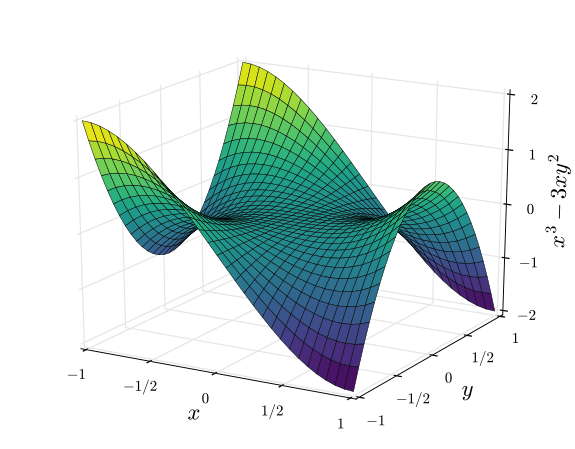
\includegraphics[scale=0.2]{sela-macaco.png}\\
	Prof. Reginaldo Demarque}



%%%%%%%%%%%%%%%%%%%%%%%%%%%%%%%%%%%%%%%%%%%%%%%%%%%%%%%%%%%%%%%%%%%%%%%%%%%%

%\pgfdeclareimage[]{logo}{uff}
%\logo{\pgfuseimage{logo}}

\logo{
\includegraphics[scale=0.03]{UFF_brasao.png}}

\institute[RCN/UFF]{Universidade Federal Fluminense\\
Instituto de Humanidades e Saúde -- RHS\\
Departamento de Ciências da Natureza -- RCN
}
\date{{\color{orange}\today}}


\frame{\titlepage}

%%%%%%%%%%%%%%%%%%%%%%%%%% sumario  %%%%%%%%%%%%%%%%%%%%%%%%%%%%%%%%

\frame{
 \frametitle{Sumário}
 \tableofcontents
}



\AtBeginSection[]
{
 \begin{frame}

  \frametitle{Sumário}
  \tableofcontents[currentsection]

 \end{frame}
}

%\includeonlyframes{otimizacao}
%bibliografia,introducao,fun-vet,funcoes,limites,der-parciais}



\section{Bibliografia}

\begin{frame}[label=bibliografia]
	\frametitle{A Disciplina}
	%\begin{scriptsize}
		\begin{block}{Bibliografia}
		
		\uncover<1->{\begin{thebibliography}{}
				
				\beamertemplatebookbibitems
				
				
				
				\bibitem[Stewart, 6\fm ed., 2011]{Stewart}
				J. Stewart
				\newblock {\em  Cálculo Volume 2}
				\newblock Editora Cengage Learning, 6\fm ed., São Paulo, 2011.
			
						
					\bibitem[Thomas, 12\fm ed., 2012]{Thomas}
				G. B. Thomas
				\newblock {\em  Cálculo Volume 2}
				\newblock Editora Pearson, 12\fm ed., São Paulo, 2012.
			\end{thebibliography}}
			
			\end{block}
	%	\end{scriptsize}
		\end{frame}
		
		\begin{frame}
\begin{block}{Bibliografia}
	
\begin{thebibliography}{}
			
			\beamertemplatebookbibitems
			
		
			
			
		\bibitem[Diomara, 3\fm ed., 2005]{Diomara}
		Diomara Pinto.  Maria Cândida Ferreira Morgado
		\newblock {\em  Cálculo Diferencial e Integral de Funções de Várias Variáveis}
		\newblock Editora UFRJ, 3\fm ed., 2005.
			
		\end{thebibliography}
		
	\end{block}
		\end{frame}
\section{Introdução}


\begin{frame}[label=introducao]
\frametitle{Introdução}

\begin{block}{Otimização de uma variável}
Imagine que você foi contratado por uma empresa que fabrica caixas sem tampa. Cada caixa é construída a partir de uma folha retangular de papelão medindo 30cm x 50cm. Para se construir uma caixa, um quadrado de lado medindo $x$ cm é retirado de cada canto da folha de papelão. O problema é determinar o valor de $x$ a fim de que a caixa correspondente tenha \dt{maior volume possível}. 
\end{block}


%\begin{center}
%\psset{unit=8mm}
%\begin{pspicture}(0,0)(7,4.5)
%\psline(1,1)(6,1)(6,4)(1,4)(1,1)
%\psline[linestyle=dashed](2,1)(2,2)(1,2)
%\psline[linestyle=dashed](5,1)(5,2)(6,2)
%\psline[linestyle=dashed](1,3)(2,3)(2,4)
%\psline[linestyle=dashed](6,3)(5,3)(5,4)
%\psline{|-|}(1,0.7)(6,0.7)
%\psline{|-|}(0.7,1)(0.7,4)
%\put(-0.5,2.5){30cm}
%\put(3,0.3){50cm}
%\psline{|-|}(6.3,3)(6.3,4)
%\psline{|-|}(5,4.3)(6,4.3)
%\put(6.4,3.5){$x$}
%\put(5.5,4.4){$x$}
%\end{pspicture}
%\end{center}

\begin{alertblock}{Problema de Maximização}
\dt{Função-objetivo:} 
\[\dt{V(x)=(30-2x)(50-2x)x}\] 
sujeito à restrição: $\dt{0\leq x\leq 15}$.
\end{alertblock}

\end{frame}



\begin{frame}

\begin{block}{Otimização de várias variáveis}
Agora imagine que você foi contratado por  uma empresa que fornece refeições a seus funcionários.
\smallskip

A fim de estabelecer um cardápio que atenda {\color{blue}a quantidade diária mínima de vitaminas} que um funcionário deve consumir  e {\color{red} minimize o custo de compras dos  diversos tipos de alimentos}.
\smallskip


Um nutricionista forneceu uma tabela que especifica a {\color{blue} quantidade mínima de cada tipo de vitamina que deve ser ingerida diariamente} por cada funcionário:
\end{block}

\begin{center}

\begin{tabu}{|l|c|c|c|c|}
\hline
Tipo de vitamina & A & B & C & E\\ \hline
	\rowfont{\color{blue}} Quantidade  mínima (mg) & 3 & 1.1 & 60 & 11\\ \hline
\end{tabu} 
\end{center}


\end{frame}

\begin{frame}
Ele também forneceu uma tabela com a quantidade (em mg) de vitaminas em cada 100 gramas de 9 tipos de alimentos diferentes,
\begin{center}
\begin{tabu}{|c|c|c|c|c|}
\hline
 Alimento & A & B & C & E  \\ \hline
1 & 0.140 & 0.08 & 0 & 1.60 \\ \hline
2 & 0.580 & 0 & 0 & 0  \\ \hline
3 & 0.150 & 1.30 & 26 & 6.90 \\ \hline
4 & 0 & 0.08 & 38 & 0.2 \\ \hline
5 & 26.780 & 0.07 & 13 & 0.07 \\ \hline
6 & 0.035 & 0.05 & 1 & 0 \\ \hline
7 & 0 & 0.04 & 5 & 0.02 \\ \hline
8 & 0 & 0.08 & 8 & 0.10 \\ \hline
9 & 0 & 0.07 & 25 & 2 \\ \hline
\end{tabu}
\end{center}

E de uma tabela com o preço de 100 gramas de cada tipo de alimento:
\begin{center}
\begin{tabu}{|c|c|c|c|c|c|c|c|c|c|}
\hline
Alimento & 1 & 2& 3 & 4 & 5 & 6 & 7 & 8 & 9\\ \hline
\rowfont{\color{red}} Preço & 0.60 & 1.00 & 5.00 & 1.00 & 0.50 & 0.20 & 0.15 & 0.40 & 1.00 \\ \hline

\end{tabu}
\end{center}
\end{frame}



\begin{frame}
 Cada alimento é uma \dt{variável de controle}, ou seja, 
 
% a variável $x_1$ representa a quantidade (em ``pacotes'' de 100g) do alimento 1 que a empresa deve comprar diariamente para cada funcionário, a variável $x_2$ representa a quantidade (em ``pacotes'' de 100g) do alimento 2 que a empresa deve comprar diariamente para cada funcionário, e assim por diante. Resumintdo, 
 
 \begin{center}
 $x_i$ representa a quantidade (em ``pacotes'' de 100g) do alimento $i$ que a empresa deve comprar diariamente para cada funcionário, com $i=1,\ldots,9$. 
 \end{center}\bigskip

A \dt{função-objetivo} que fornece o custo (que queremos minimizar) associado à compra  dos diversos tipos de alimentos para cada funcionário é dada por 
\begin{multline*}
C(x_1,x_2,x_3,x_4,x_5,x_6,x_7,x_8,x_9)= \\ {\color{red}0.6}x_1 + {\color{red} 1}x_2 +{\color{red} 5}x_3+{\color{red} 1}x_4+{\color{red} 0.5}x_5+{\color{red} 0.2}   x_6+{\color{red} 0.15}x_7+{\color{red} 0.4}x_8+{\color{red} 1}x_9.
\end{multline*}


\end{frame}



\begin{frame}
\frametitle{ }

Consultando as outras tabelas, podemos ver que o problema está sujeito às restrições impostas pelas quantidades mínimas de cada vitamina, a saber

\begin{small}
\begin{align*}
&0.14x_1+0.58x_2+0.15x_3+26.79x_5+0.035x_6\geq {\color{blue} 3},\\
&0.08x_1+1.3x_3+0.08x_4+0.07x_5+0.05x_6+0.04x_7+0.08x_8+0.07x_9\geq {\color{blue} 1.1},\\
&26x_3+38x_4+13x_5+x_6+5x_7+8x_8+25x_9\geq {\color{blue} 60},\\
&1.6x_1+6.9x_3+0.2x_4+0.07x_5+0.02x_7+0.1x_8+2x_9\geq {\color{blue} 11},\\
&x_i\geq {\color{blue} 0}, \ \forall i=1,\ldots,9.
\end{align*} 
\end{small}

\uncover<1->{Usando as técnicas que serão vistas neste curso de cálculo 3 é possível resolver este problema e obter a seguinte solução:
$$x_1=6.24,\  x_3=0.112, \ x_5=0.078,\ x_7=11.209$$
$$ x_2=x_4=x_6=x_8=x_9=0$$ }

\end{frame}

\begin{frame}
	\begin{casa}
		Revise as seções 12.5 e 12.6 do \cite{Stewart} e faça seguintes os exercícios
		\begin{enumerate}
			\item Determine as equações paramétricas da reta que passa pelos pontos $A=(1,3,2)$ e $B=(-4,3,0)$
			
			\item Determine a equação do plano que passa pelo ponto $A=(6,3,2)$ e é perpendicular ao vetor $\vec{n}=(-2,1,5)$
				
		\item Identifique e esboce as superfícies:
		\begin{enumerate}[a]
			\item $x^2+y^2+z^2=4$
			\item $z^2=y^2+4x^2$
			\item $z=x^2+y^2$
		\end{enumerate}
		
		\end{enumerate}
	\end{casa}
\end{frame}
\section{Funções Vetoriais}

\subsection*{Definição de funções Vetoriais}
\begin{frame}[label=fun-vet]{Funções Vetoriais}
\begin{defin}
Uma \dt{função vetorial} é uma função cujo domínio é um conjunto de números reais e cuja imagem é um conjunto de vetores em $\R^n$, denotada por:
\[\begin{array}{lcl}
\vec{r}: & D\subset \R &  \longrightarrow \R^n\\
         & t           & \longmapsto \vec{r}(t)=(f_1(t),f_2(t),\ldots,f_n(t)).
\end{array}\]

As funções $f_1,\ldots,f_n$ são chamada \dt{funções componentes}.
\end{defin}

\begin{example}
\begin{enumerate}
\item $\vec{r}(t)=(t,t)$, $t\in \R$.
\item $\vec{r}(t)=(t,1,0)$, $t\geq 0$.
\end{enumerate}
\end{example}

\end{frame}


\subsection*{limite e continuidade}
\begin{frame}[label=fun-vet]{Limite e Continuidade}
\begin{defin}
Sejam $\vec{r}(t)=(f_1(t),f_2(t),\ldots,f_n(t))$ uma função vetorial com domínio $D$. Definimos o \dt{limite de $\vec{r}(t)$ quanto $t$ tende a $a\in D$} por 
\[\lim\limits_{t\to a}\vec{r}(t)=\left(\lim\limits_{t\to a}f_1(t),\ldots,\lim\limits_{t\to a}f_n(t)\right), \]
desde que o limite das funções componentes existam.
\end{defin}

\begin{exer}
Determine $\lim\limits_{t\to 0}\vec{r}(t)$, onde $\vec{r}(t)=(1+t^3, te^{-t})$.
\end{exer}


\end{frame}

\begin{frame}[label=fun-vet]
\begin{defin}
Uma função vetorial $\vec{r}$ é \dt{contínua em $a$} se $\lim\limits_{t\to a}\vec{r}(t)=\vec{r}(a)$.
\end{defin}
Em vista desta definição, uma função $\vec{r}$ é {\color{blue}contínua em $a$} se, e somente se, cada uma de suas {\color{blue}componentes é contínua em $a$}.



\end{frame}

\subsection*{Curvas Parametrizadas}
\begin{frame}[label=fun-vet]{Curvas Parametrizadas no plano}
Quando uma função vetorial \dt{$\vec{r}(t)=(f(t),g(t))$}, está definida em um intervalo $I$ da reta e  é \dt{contínua}, então o conjunto {\color{red}$C$} de todos os pontos $(x,y)$ do plano tais que
\begin{equation}\label{parametricas}
x=\dt{f(t)}\ \text{ e } y=\dt{g(t)}
\end{equation}
quando $t$ varia formam uma {\color{red}curva no plano}. As equações em  {\color{red} \eqref{parametricas}} são ditas {\color{red} equações paramétricas de $C$}, $\dt{\vec{r}}$ é dita ser uma {\color{red}parametrização de $C$} e $t$ é chamado de  {\color{red} Parâmetro}.
\begin{exe}
Determine as curvas parametrizadas por:
\begin{enumerate} 
\item $\vec{r}(t)=(\cos(t),\sin(t))$, $t\in [0,2\pi]$.
\item $\vec{r}(t)=(\cos(2t),\sin(2t))$, $t\in [0,2\pi]$.

\end{enumerate}
\end{exe}

Veja como plotar curvas parametrizadas usando python \href{https://reginaldodr.github.io/academic/posts/curvas-parametricas/curvas-parametricas.html}{\beamergotobutton{Link}}

\end{frame}

\begin{frame}[label=fun-vet]
\begin{block}{Parametrização de Função}
O gráfico de qualquer função $y=f(x)$ pode ser parametrizado de forma natural usando a variável $x$ como parâmetro, da seguinte forma:
\[\vec{r}(t)=(t,f(t)),\ t\in I.\]
\end{block}

\begin{exer}
 Determine uma parametrização para a parábola $y=x^2$.
\end{exer}
\end{frame}


\begin{frame}[label=fun-vet]
	\begin{casa}
		\begin{enumerate}
			\item  Determine uma parametrização para o segmento de reta que entre os pontos $(1,0)$ e $(2,5)$.
			\item Determine a curva parametrizada por $\vec{r}(t)=(2\cos(t),\sin(t))$, $t\in [0,2\pi]$.
		\end{enumerate}
	\end{casa}
\end{frame}

%---------------  coordenadas polares



\begin{frame}[label=fun-vet]{Coordenadas Polares}

		Um sistema de \dt{coordenadas polares} é estabelecido ao escolhermos um ponto no plano, conhecido como \dt{polo} (ou origem), denotado por $O$, e uma semi-reta começando em $O$, chamada \dt{eixo polar}. Qualquer ponto $P$ do plano é associado a um par ordenado $(r,\theta)$, chamado \dt{coordenadas polares} de $P$, sendo $r$ a distância de $P$ a $O$ e $\theta$ o ângulo entre o eixo polar e a reta $OP$.
		\medskip

\centering
\begin{tikzpicture}
\tikzset{>=latex}

\coordinate (A) at ({2*cos(45)},{2*sin(45)});
\coordinate (O) at (0,0);
\coordinate (i) at (2,0);

\pic[draw,angle eccentricity=1.5,->] {angle = i--O--A};

\draw[->] (0,0) -- (3,0) node[right] {eixo polar};

\node[thick] at (0.8,0.3) {$\theta$};
\draw[very thick,blue] (0,0) -- ({2*cos(45)},{2*sin(45)});

\node at (0.5,1) {$r$};
\node[right] at (A) {$(r,\theta)$};
\fill[red] (A) circle (2pt);

\node[left] at (0,0) {$O$};
  
\end{tikzpicture}


		\end{frame}
		

\begin{frame}[label=fun-vet]{Coordenadas Polares}
Usamos a convenção de que um ângulo é positivo se for medido no sentido anti-horário a partir do eixo polar e negativo se for medido no sentido horário. Se $P=O$, então $r=0$, e convencionamos que $(0,\theta)$ representa o polo para qualquer valor de $\theta$.
\medskip

No caso $r<0$, convencionamos que a coordenada $(r,\theta)$ corresponde ao simétrico, em relação à origem, do ponto $(|r|,\theta)$.

\centering

\begin{tikzpicture}
\tikzset{>=latex}

\coordinate (A) at ({2*cos(45)},{2*sin(45)});
\coordinate (O) at (0,0);
\coordinate (i) at (2,0);
\coordinate (B) at ({2*cos(45+180)},{2*sin(45+180)});

\pic[draw,->,angle radius=1cm] {angle = i--O--A};

\pic[draw,->] {angle = i--O--B};

\draw[->] (0,0) -- (3,0) node[right] {eixo polar};

\node[thick] at (1.2,0.3) {$\theta$};
\draw[very thick,dashed] (0,0) -- ({2*cos(45)},{2*sin(45)});

\node at (0.5,1) {$r$};
\node[right] at (A) {$(r,\theta)$};
\fill[black] (A) circle (2pt);

\node[below] at (0,0) {$O$};

\draw[very thick,blue] (0,0) -- ({2*cos(45+180)},{2*sin(45+180)});

\node[left] at (B) {$(-r,\theta)$};
\fill[red] (B) circle (2pt);
\node at ({0.8*cos(90+45)},{0.8*sin(90+45)}) {$\theta +\pi$};
  
\end{tikzpicture}



\end{frame}
		
		\begin{frame}[label=fun-vet]
				\begin{exe}
					Marque os pontos cujas coordenadas polares são dadas
					\begin{multicols}{4}
						\begin{enumerate}[a]
							\item $(1,5\pi/4)$
							
							\item $(2,3\pi)$
							
							\item  $(2,-2\pi/3)$
							
							\item $(-3,3\pi/4)$  \medskip
						\end{enumerate}
					\end{multicols}
				\end{exe}

\begin{center}
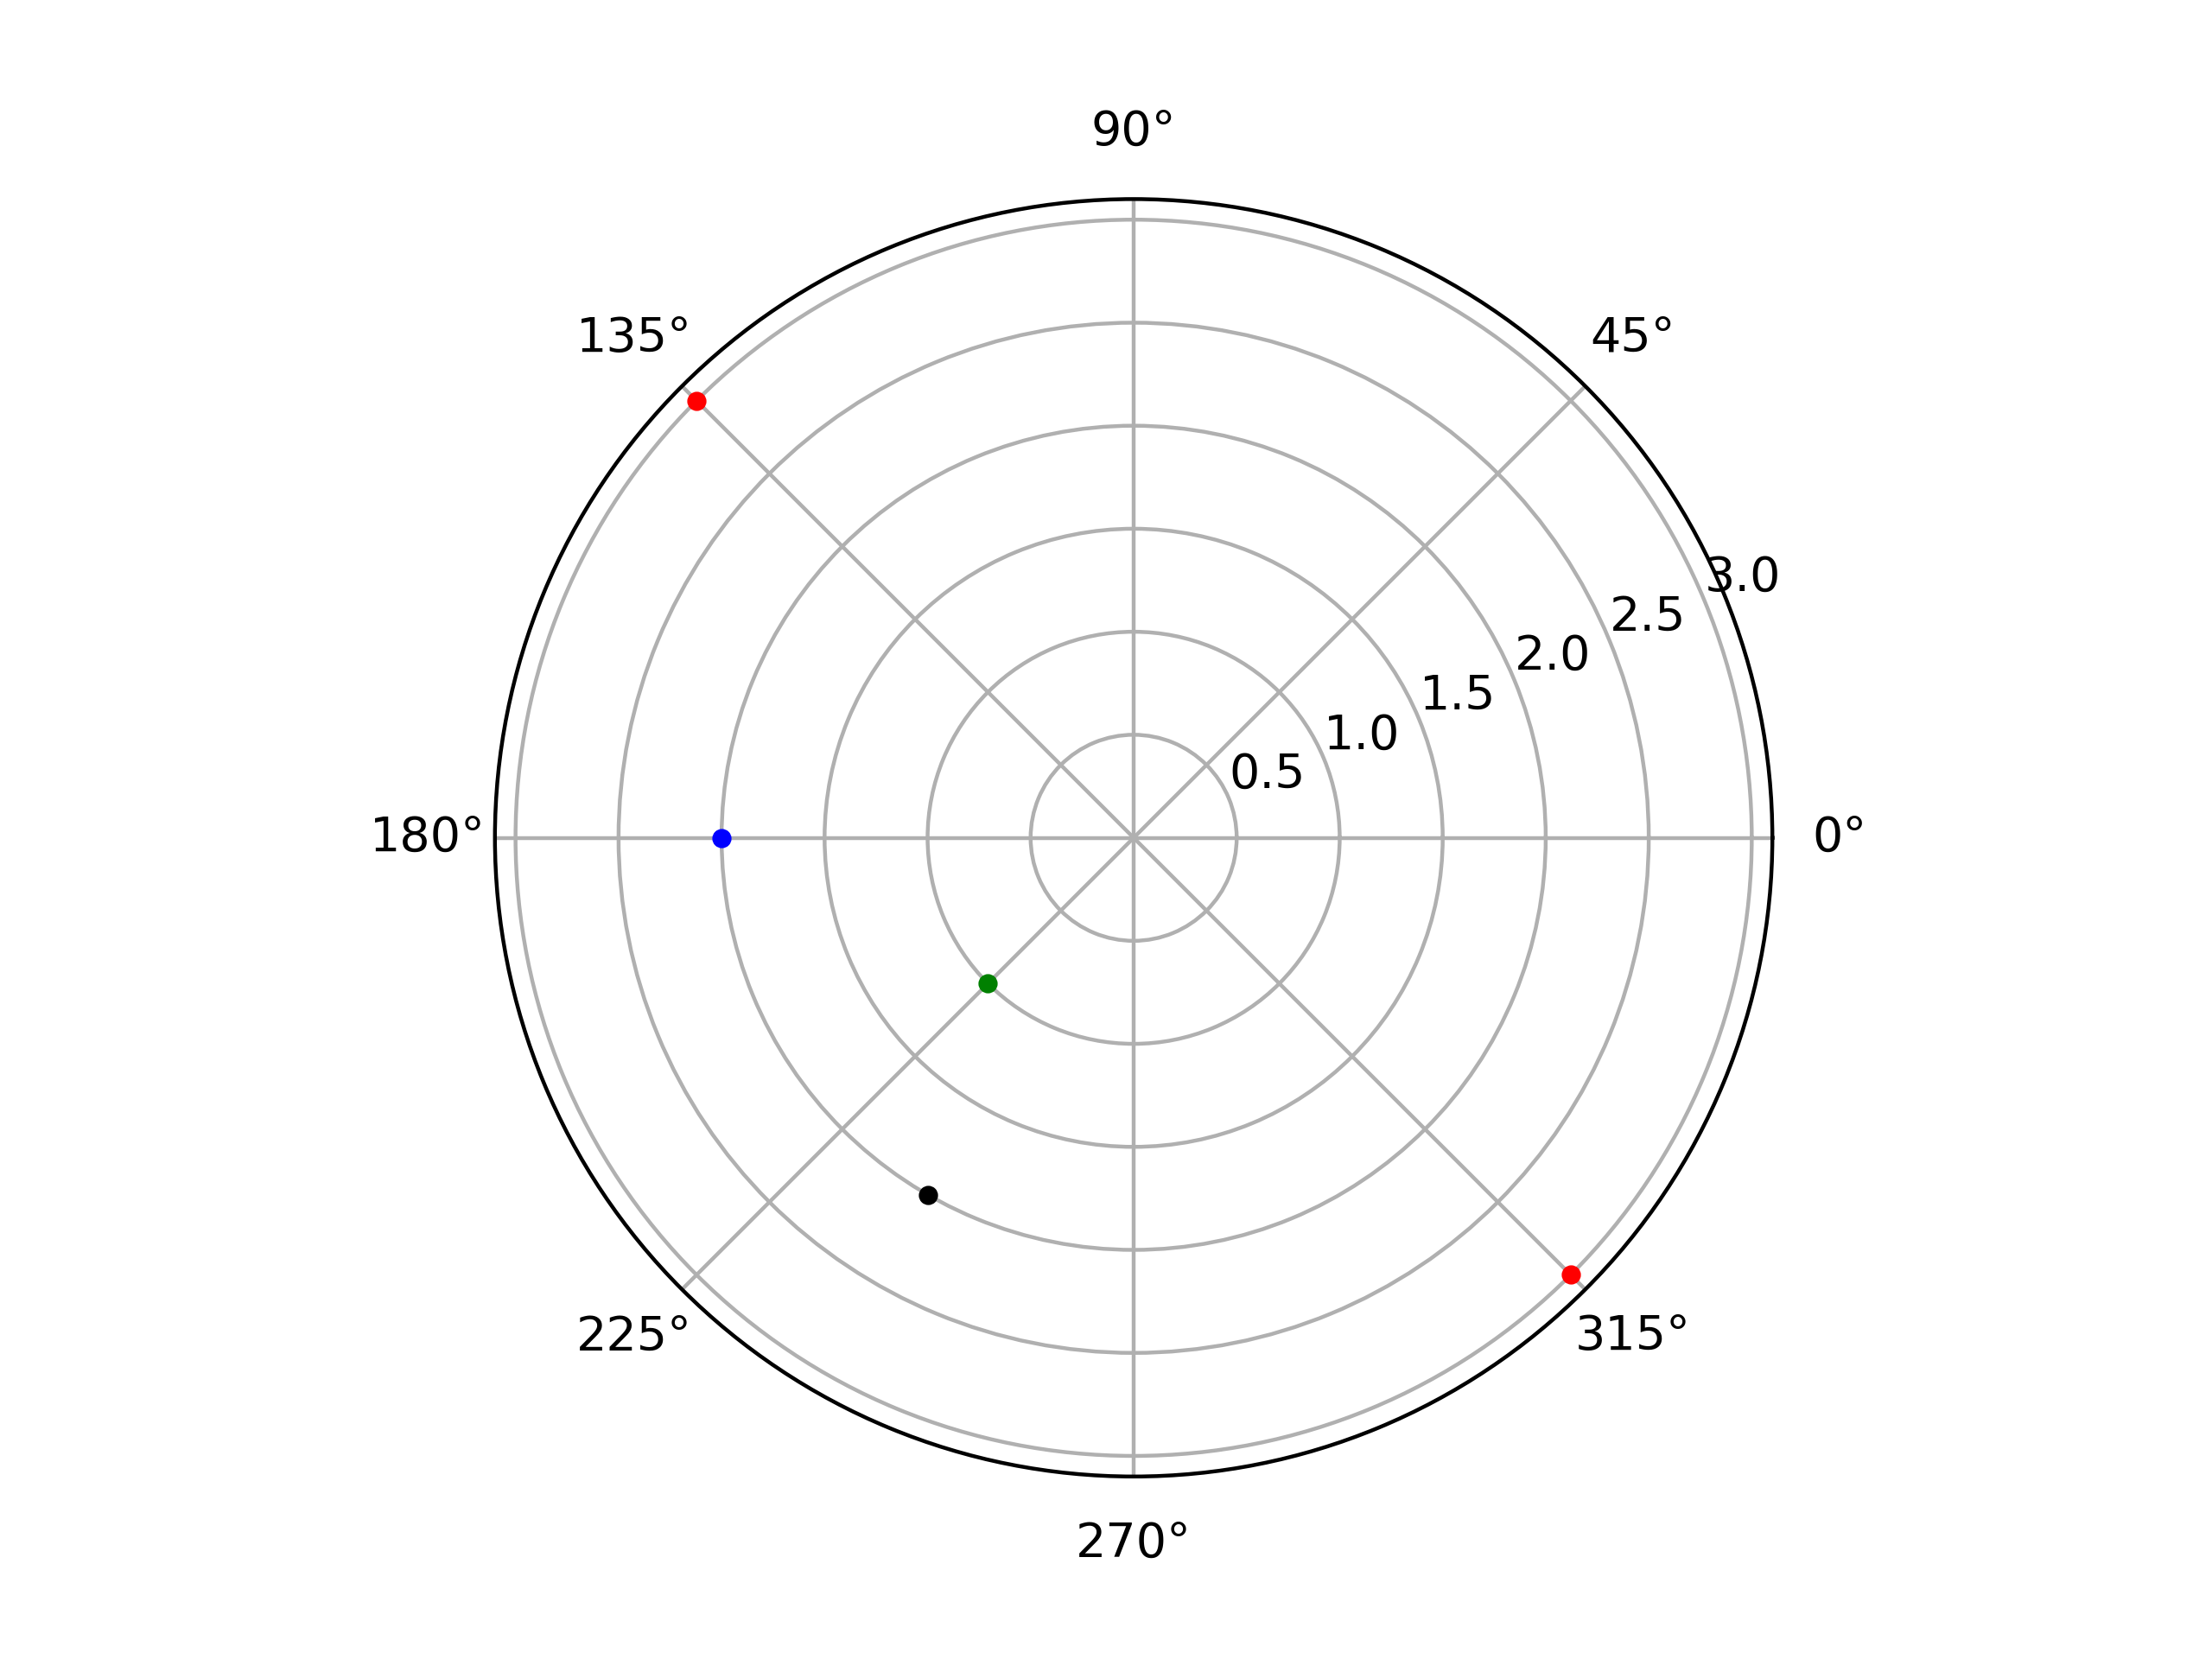
\includegraphics[scale=.5]{figuras/polar1.png}
\end{center}

		\end{frame}

\begin{frame}[label=fun-vet,fragile=singleslide]
\begin{block}{ }
\begin{pyverbatim}
import numpy as np
import matplotlib.pyplot as plt
  
plt.axes(projection = 'polar')

plt.polar(5*np.pi/4,1, 'g.')
plt.polar(3*np.pi,2, 'b.')
plt.polar(-2*np.pi/3,2, 'k.')
plt.polar(3*np.pi/4,3, 'r.')
plt.polar(3*np.pi/4+np.pi,3, 'r.')
   
plt.show()
\end{pyverbatim}
\end{block}


\end{frame}



\begin{frame}[label=fun-vet]{Curvas Polares}
\begin{block}{Relação entre coordenadas cartesianas e polares}

$$x=r\cos \theta, \ \ \ y=r\sen \theta, \ \ \ r^2=x^2+y^2$$
\end{block}

O \dt{gráfico de uma equação polar} consiste em todos os pontos $P$ que têm pelo menos uma representação $(r,\theta)$ cujas coordenadas satisfaçam a equação. 

\begin{exe} Esboce a curva que é representada pelas equações polares abaixo.
%\begin{multicols}{3}
		\begin{enumerate}[a]
		\item $r=2$
		
		\item $\theta=1$
		
%		\item $r=2\cos\theta$

	%	\item $r=1+\cos\theta$ (cardioide)
%		\item $r=\cos 2\theta$ (rosácea de quatro pétalas)
			\end{enumerate}
%\end{multicols}
\end{exe}

\end{frame}

\begin{frame}[label=fun-vet]
\begin{exe} Esboce a curva que é representada pela seguinte equação polar
\[r=1+\cos\theta \text{ (cardioide)}\]
\end{exe}


\begin{center}
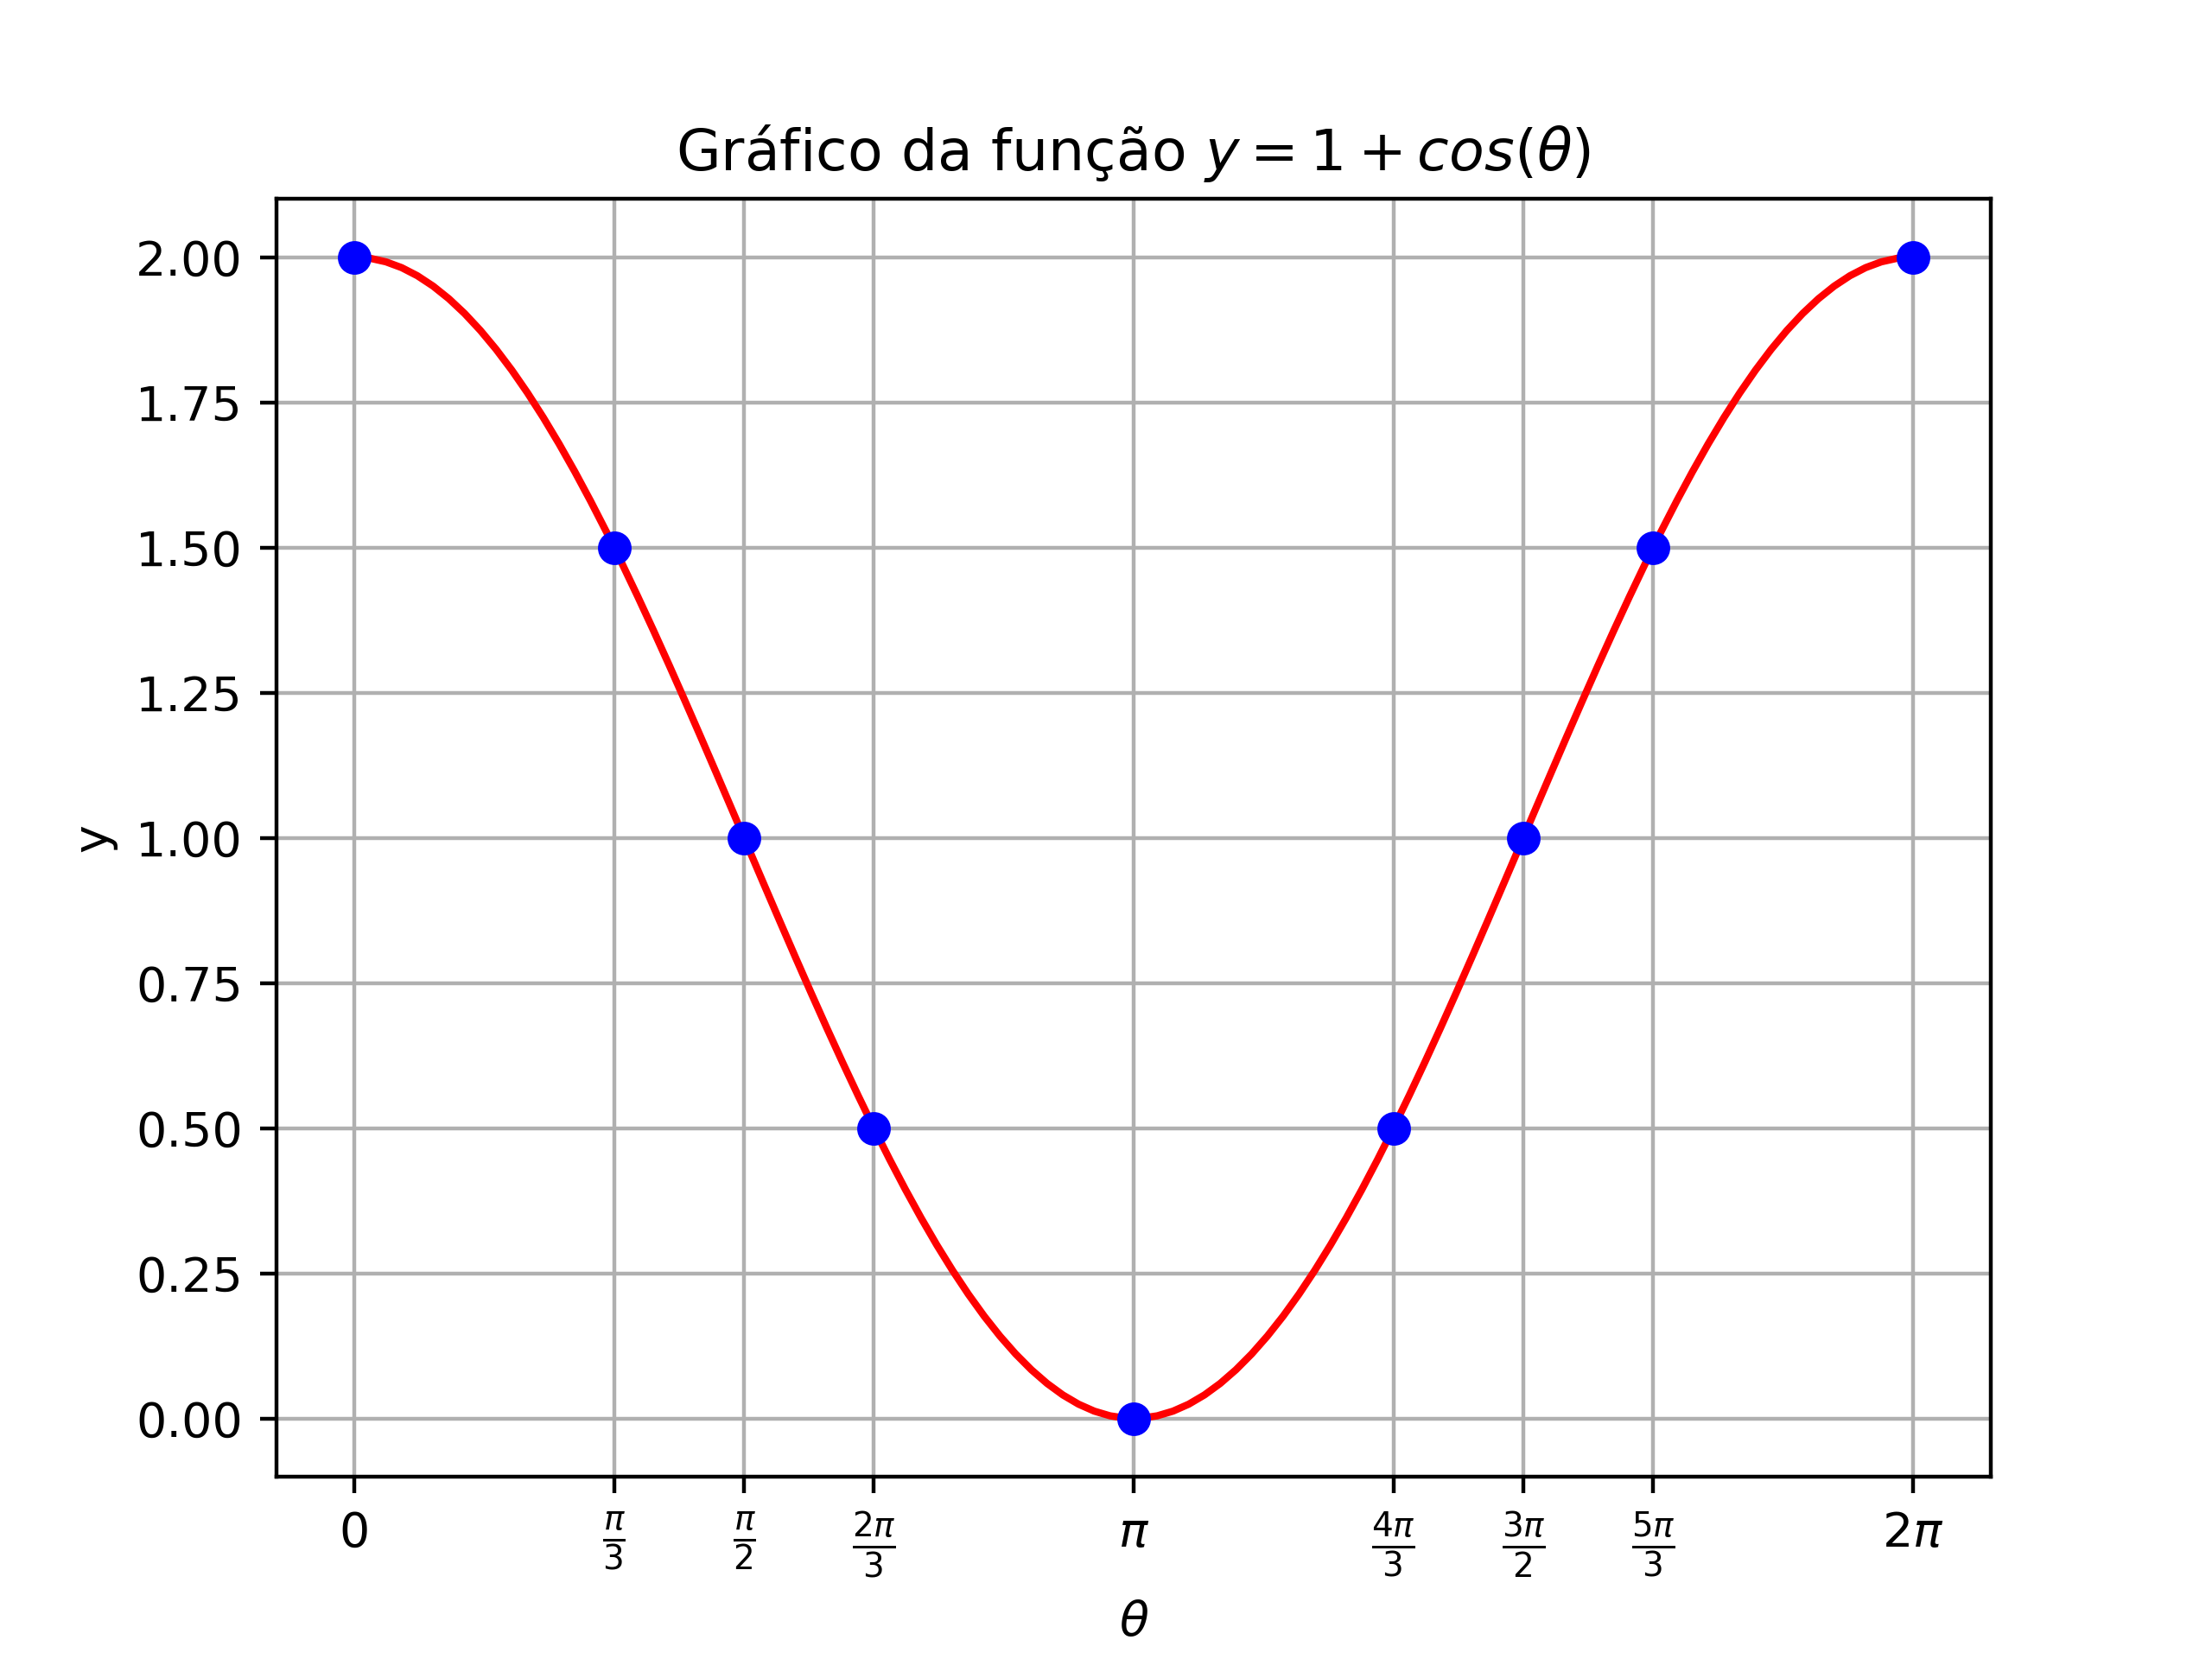
\includegraphics[scale=0.5]{figuras/grafico-aux-cardioide.png}
\end{center}
\end{frame}

\begin{frame}[label=fun-vet,fragile=singleslide]
\begin{block}{ }
\begin{pyverbatim}
import matplotlib.pyplot as plt
import numpy as np

theta= np.linspace(0, 2*np.pi, 60)
r=1+np.cos(theta)

theta=np.where(r >= 0, theta,theta + np.pi)

plt.polar(theta, np.abs(r))
plt.show()
\end{pyverbatim}
\end{block}


\end{frame}


\begin{frame}[label=fun-vet]
%\only<1>{\begin{figure}
%\centering
%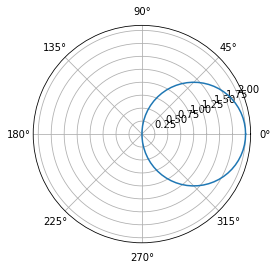
\includegraphics[scale=.7]{figuras/polar-circ.png}
%\caption{$r=2\cos \theta$}
%\end{figure}}
\only<1>{\begin{figure}
\centering
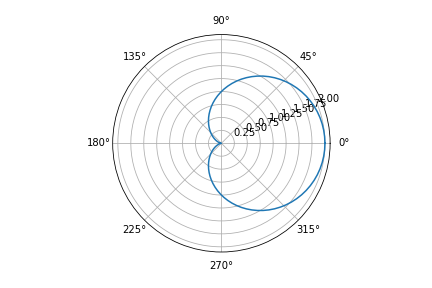
\includegraphics[scale=.7]{figuras/polar-card.png}
\caption{$r=1+\cos\theta$}
\end{figure}}
%\only<3>{\begin{figure}
%\centering
%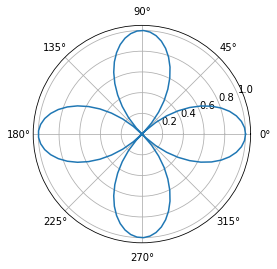
\includegraphics[scale=.7]{figuras/polar-rosasea.png}
%\caption{$r=\cos 2\theta$}
%\end{figure}}
\end{frame}

\begin{frame}[label=fun-vet]{Usando coordenadas Polares para Parametrizar}
Se em uma equação polar conseguirmos escreve a coordenada $r$ em função de $\theta$, isto é, $r=f(\theta)$, então podemos usar $\theta$ como parâmetro e parametrizar a curva representada pela equação polar da seguinte forma:
\[\vec{\alpha}(\theta)=f(\theta)(\cos \theta,\sin \theta)\]

\begin{exe}
Uma parametrização da cardioide $r=1+\cos \theta$ 
\[\vec{\alpha}(\theta)=(r\cos \theta,r\sin \theta)=(1+\cos (\theta))(\cos \theta,\sin \theta),\ \theta\in [0,2\pi].\]

\end{exe}
\end{frame}

\begin{frame}[label=fun-vet]
	\begin{casa}
		
		Esboce a curva que é representada pelas equações polares abaixo.
\begin{enumerate}
\item $r=2\cos\theta$
	
\item $r=\cos 2\theta$ (rosácea de quatro pétalas)
\end{enumerate}
	\end{casa}
\end{frame}


%\begin{frame}[label=fun-vet]
%	\begin{casa}
%		 Faça os seguintes exercícios da seção 10.3 de \cite{Stewart}
%			1, 3, 7, 9, 11, 15, 17, 19, 21, 23, 25, 29, 31, 33, 35, 37, 39, 41. 
%	
%	\end{casa}
%\end{frame}




%------------------------------------------

\begin{frame}[label=fun-vet]{Curvas Parametrizadas no espaço}
Quando uma função vetorial \dt{$\vec{r}(t)=(f(t),g(t),h(t))$}, está definida em um intervalo $I$ da reta e  é \dt{contínua}, então o conjunto {\color{red}$C$} de todos os pontos $(x,y,z)$ do plano tais que
\begin{equation}\label{parametricas2}
x=\dt{f(t)},\  y=\dt{g(t)}\ \text{ e } z=\dt{h(t)}
\end{equation}
quando $t$ varia formam uma {\color{red}curva no espaço}. As equações em  {\color{red} \eqref{parametricas2}} são ditas {\color{red} equações paramétricas de $C$}, $\dt{\vec{r}}$ é dita ser uma {\color{red}parametrização de $C$} e $t$ é chamado de  {\color{red} Parâmetro}.
\begin{exe}
Determine as curvas parametrizadas por:
\begin{enumerate} 
\item $\vec{r}(t)=(1,t,2t)$, $t\in (0,1)$.
\item $\vec{r}(t)=(\cos(t),\sin(t),t)$, $t\in [0,2\pi]$.
\end{enumerate}
\end{exe}


Veja como plotar curvas parametrizadas usando python \href{https://reginaldodr.github.io/academic/posts/curvas-parametricas/curvas-parametricas.html}{\beamergotobutton{Link}}

\end{frame}

\begin{frame}[label=fun-vet]
\begin{block}{Hélices}
A curva do exemplo anterior é uma \dt{hélice}. Existem vários tipos de hélices, as mais simples são as \dt{hélices circulares com passo constante}, cuja  parametrização e dada por 
\[\vec{r}(t)=({\color{red}a}\cos(t),{\color{red}a}\sin(t),{\color{blue}b}t),\]
onde ${\color{red}a},{\color{blue}b}$ são constantes.

As hélices aparecem em diversas aplicações, como por exemplo no formato de molas e no modelo de DNA que é formado por uma dupla hélice.
\end{block}
\begin{minipage}{0.3\textwidth}
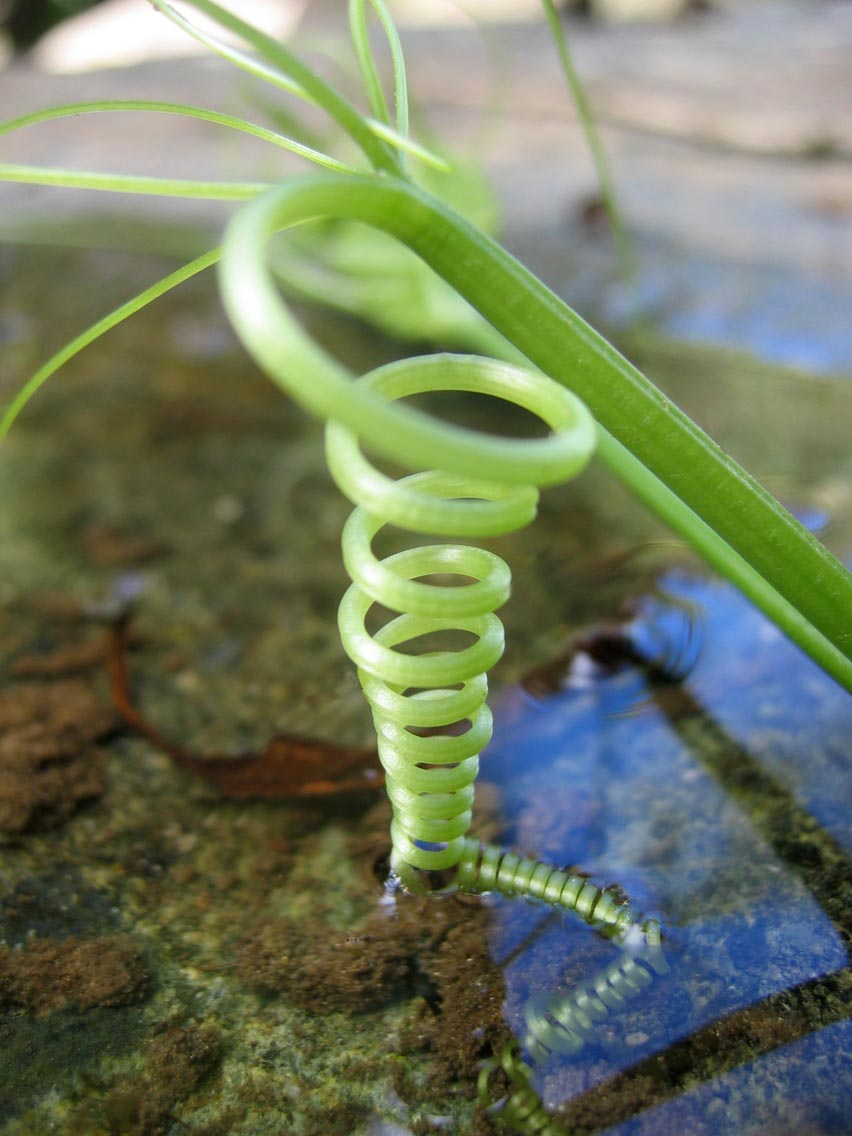
\includegraphics[scale=0.1]{figuras/DirkvdM_natural_spiral.jpg}
\end{minipage}
\begin{minipage}{0.35\textwidth}
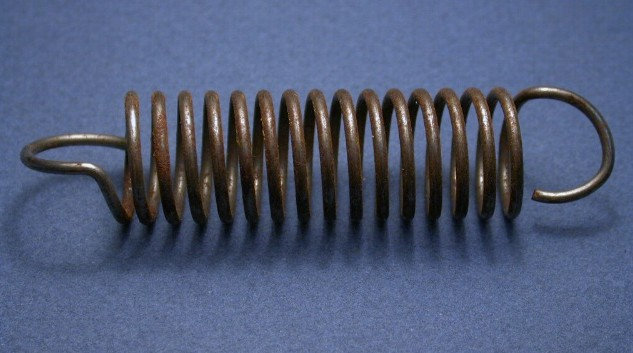
\includegraphics[scale=.7]{figuras/mola.jpg}
\end{minipage}
\begin{minipage}{0.3\textwidth}

\includegraphics[scale=.4]{figuras/dna.png}
\end{minipage}

\end{frame}



\begin{frame}[label=fun-vet]
\begin{casa}
\begin{enumerate}
\item Determine uma parametrização para o círculo de centro em $(1,2)$ e raio $3$.
\item Determine uma parametrização para o segmento de reta ligando o ponto $P=(1,3,-2)$ ao ponto $Q=(2,-1,3)$.

\item Calcule $\|\vec{r}(t)\|$, onde $\vec{r}(t)=(\cos t,\sin t, t)$, $t\in \R$.

\item Determine uma equação vetorial que represente a curva obtida pela interseção do cilindro $x^2+y^2=1$ com o plano $y+z=2$.
\item Mostre que a curva $\vec{r}(t)=(t\cos t,t\sin t,t)$ está contida no cone $z^2=x^2+y^2$ e use esse fato para esboçar a curva.
\end{enumerate}
\end{casa}
\end{frame}

\subsection*{Derivadas}
\begin{frame}[label=fun-vet]{Derivadas}
\begin{defin}
A \dt{derivada} de uma função vetorial $\vec{r}$ é definida por:
\[\frac{d\vec{r}}{dt}=\vec{r}\,'(t)=\lim\limits_{h\to 0}\frac{\vec{r}(t+h)-r(t)}{h},\]
se esse limite existir.
\end{defin}
\begin{block}{Interpretação Geométrica}
O vetor $\vec{r}\,'(t)$ é um \dt{vetor tangente} à curva parametrizada por $\vec{r}$ no ponto $P=\vec{r}(t)$.
\end{block}


\end{frame}

\begin{frame}[label=fun-vet]
\begin{prop}
Se $\vec{r}(t)=\left(f_1(t),\ldots,f_n(t)\right)$, onde $f_i$, com $i=1,\ldots,n$, são funções deriváveis, então
\[\vec{r}\,'(t)=\left(f_1'(t),\ldots,f_n'(t)\right)\]
\end{prop}

\begin{exe}
Encontre o vetor tangente unitário no ponto $t=0$ da curva 
\[\vec{r}(t)=\left(1+t^3,te^{-t},\sin(2t)\right).\]
\end{exe}
\end{frame}

\subsection*{Regras de Derivação}
\begin{frame}[label=fun-vet]{Regras de Derivação}
\begin{prop}
Sejam $\vec{u}$ e $\vec{v}$ funções vetoriais diferenciáveis, $c$ uma constante e $f$ uma função real. Então,
\begin{enumerate}
\item $\frac{d}{dt}\left(\vec{u}(t)+\vec{v}(t)\right)= \vec{u}\,'(t)+\vec{v}\,'(t)$
\item $\frac{d}{dt}\left(c\vec{u}(t)\right)= c\vec{u}\,'(t)$
\item $\frac{d}{dt}\left(f(t)\vec{u}(t)\right)= f'(t)\vec{u}(t)+f(t)\vec{u}\,'(t)$
\item $\frac{d}{dt}\left(\vec{u}(t)\cdot \vec{v}(t)\right)= \vec{u}\,'(t)\cdot\vec{v}(t)+\vec{u}(t)\cdot\vec{v}\,'(t)$
\item $\frac{d}{dt}\left(\vec{u}(t)\times \vec{v}(t)\right)= \vec{u}\,'(t)\times\vec{v}(t)+\vec{u}(t)\times\vec{v}\,'(t)$
\item $\frac{d}{dt}\left(\vec{u}(f(t))\right)= f'(t)\vec{u}\,'(f(t))$ (regra da cadeia)
\end{enumerate}
\end{prop}


\end{frame}


\begin{frame}[label=fun-vet]
\begin{exe}
Mostre que se $\|\vec{r}(t)\|=c$ para todo $t\in I$, então $\vec{r}\,'(t)$ é ortogonal a $\vec{r}(t)$ para todo $t\in I$.
\end{exe}

\begin{center}
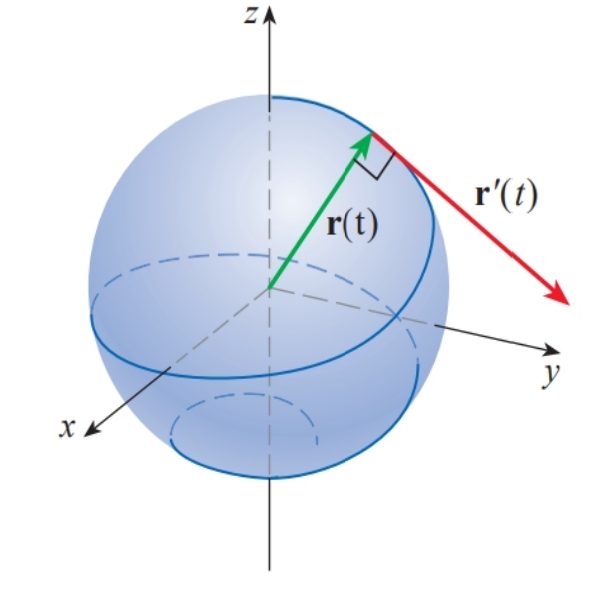
\includegraphics[scale=0.4]{figuras/vetor-const.png}
\end{center}
\end{frame}

%
%\subsection*{Integrais}
%\begin{frame}{Integral}
%A \dt{integral definida} de uma função vetorial contínua $\vec{r}$ pode ser definida da seguinte forma:
%\begin{equation*}
%	\begin{split}
%\int_a^b \vec{r}(t)\, dt & =\lim\limits_{m\to \infty}\sum_{i=1}^{m}\vec{r}(t_i^\ast)\Delta t\\
%& =\lim\limits_{m\to \infty}\left(\sum_{i=1}^{m}f_1(t_i^\ast)\Delta t,\sum_{i=1}^{n}f_2(t_i^\ast)\Delta t,\ldots,\sum_{i=1}^{n}f_n(t_i^\ast)\Delta t\right)\\
%& =\left(\int_{a}^{b}f_1(t)\,dt,\int_{a}^{b}f_2(t)\,dt,\ldots,\int_{a}^{b}f_n(t)\,dt\right)
%	\end{split}
%\end{equation*}
%\begin{exer}
%	Calcule a integral de $\vec{r}(t)=\left(2\cos(t),\sin(t)\right)$ em $[0,\pi/2]$.
%\end{exer}
%
%
%\end{frame}

\subsection*{Comprimento de arco}


\begin{frame}[label=fun-vet]{Comprimento de Arco}
	 Se {\color{red}$\vec{r}=\vec{r}(t)$}, com $a\leq t\leq b$, é curva parametrizada e {\color{red}$\vec{r}\,^\prime$ } é contínua, pode-se mostrar que o \dt{comprimento de arco} é dado por:
	\[\dt{L}=\int_a^b\|{\color{red}\vec{r}\,'(t)}\|\,dt\]
	\begin{exe}
		Um planador está voando para cima ao longo da hélice $\vec{r}(t)=(\cos(t),\sin(t),t)$. Qual a distância percorrida ao longo de sua trajetória entre os pontos $(1,0,0)$ e $(1,0,2\pi)$.
	\end{exe}
 \end{frame}


\begin{frame}
Uma mesma curva $C$ pode ser representada por mais de uma parametrização. Por exemplo, 
\[\vec{\alpha}(t)=(\cos(t),\sin(t)),\ 0\leq t\leq 2\pi\]
e
\[\vec{\beta}(t)=(\cos(2t),\sin(2t)),\ 0\leq t\leq \pi\]
ambas representam o círculo unitário com centro na origem. 

\begin{exer}
Calcule o comprimento de arco de $\vec{\alpha}=\vec{\alpha}(t)$ e $\vec{\beta}=\vec{\beta}(t)$.
\end{exer}
\end{frame}


\subsection*{Parametrização Pelo Comprimento de Arco}
\begin{frame}[label=fun-vet]{Função Comprimento de Arco}
Seja $C$ uma curva parametrizada por $\vec{r}=\vec{r}(t)$, $a\leq t\leq b$, onde $\vec{r}\,^\prime$ é contínua. Definimos a sua {\color{blue} função comprimento de arco} por
\[s(t)=\int_a^t\|\vec{r}\,^\prime (u)\|du.\]

Note que 
\[\frac{ds}{dt}=\|\vec{r}\,^\prime (t)\|\geq 0,\]
assim $s=s(t)$ é uma {\color{red}função crescente} e de classe $C^1$. Neste caso, $s$ possui uma inversa, denotada por $t=t(s)$.

\end{frame}


\begin{frame}[label=fun-vet]{Parametrização pelo Comprimento de Arco}
Isso nos permite {\color{red} reparametrizar a curva $C$ em relação ao comprimento de arco} fazendo
\[\vec{r}(s)=\vec{r}(t(s)),\ 0\leq s\leq L,\]
onde $L$ é o comprimento final da curva.

\begin{block}{ }
É frequentemente útil usar a parametrização em relação ao comprimento de arco, pois este não depende do sistema de coordenadas nem da parametrização.
\end{block}
\end{frame}

\begin{frame}[label=fun-vet]
\begin{exe}
Reparametrize a hélice circular $\vec{r}(t)=(\cos(t),\sin(t),t)$ utilizando o comprimento de arco a partir do ponto $(1,0,0)$.
\end{exe}


\begin{block}{}
Quando a curva está parametrizada pelo comprimento de arco, geometricamente isso significa que o ponto $\vec{r}(s)$  é o ponto da curva que está a $s$ unidades de comprimento do início da curva.
\end{block}
\end{frame}

\begin{frame}[label=fun-vet]
\begin{casa}
Seja $\vec{r}(t)=(e^t\sin(t),e^t\cos(t),\sqrt{2}e^t)$ e $P=(0,1,\sqrt{2})$. 
\begin{enumerate}
\item Encontre a função comprimento de arco da curva medida a partir do ponto $P$ na direção crescente de $t$.
\item Reparametrize a curva com relação ao comprimento de arco começando de $P$.
\item Encontre o ponto a 4 unidades de $P$ ao longo da curva na direção crescente de $t$.
\end{enumerate}
\end{casa}
\end{frame}

\subsection*{Curvatura}
\begin{frame}[label=fun-vet]{Vetor Tangente Unitário}
Uma parametrização {\color{red} $\vec{r}=\vec{r}(t)$} é chamada {\color{blue} suave} em um intervalo $I$ se {\color{red}$\vec{r}\,^\prime$} for contínua e {\color{red}$\vec{r}\,^\prime(t)\neq \vec{0}$} em $I$.
\medskip

Se $C$ é uma curva parametrizada por $\vec{r}=\vec{r}(t)$ suave, então o {\color{blue}vetor tangente unitário} é definido por:
\[\vec{T}(t)=\frac{\vec{r}\,^\prime(t)}{\|\vec{r}\,^\prime(t)\|}.\]


\begin{minipage}{0.5\textwidth}
O vetor tangente unitário indica a direção da curva e muda de direção muito devagar quando a curva $C$ é razoavelmente reta, mas muda mais rapidamente quando se dobra mais acentuadamente.
\end{minipage}
\begin{minipage}{0.4\textwidth}
\begin{center}
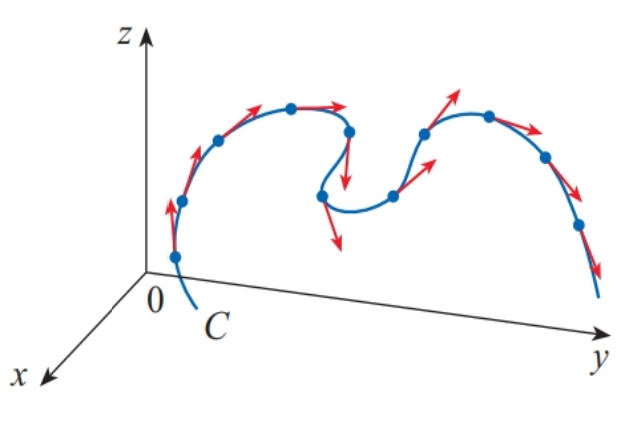
\includegraphics[scale=0.35]{figuras/vetor-tangente.png}
\end{center}
\end{minipage}

\end{frame}


\begin{frame}[label=fun-vet]{Curvatura}
A {\color{blue}curvatura} de $C$ em dado ponto é definida como 

\begin{center}
{\color{red}a taxa de variação da direção do vetor tangente unitário por unidade de comprimento,}
\end{center}
em outras palavras,
\begin{center}
{\color{red} a medida de quão rapidamente a curva muda de direção no ponto}.
\end{center} 

Por isso, definimos a curvatura como a norma  da taxa de variação do vetor tangente unitário com relação ao comprimento de arco, a saber, 
\[
\kappa(s)=\left\|\frac{d\vec{T}(s)}{ds}\right\|,
\]
onde $\vec{T}$ é o vetor tangente unitário.
\end{frame}

\begin{frame}[label=fun-vet]
Entretanto, na maioria das vezes a curva não está parametrizada pelo comprimento de arco. Neste caso, podemos usar a Regra da Cadeia para obter uma fórmula em termos de um parâmetro qualquer. Se $s=s(t)$ é a função comprimento de arco, então:
\[\frac{d\vec{T}(s(t))}{dt}=\frac{d\vec{T}(s)}{ds}\frac{ds}{dt}=\frac{d\vec{T}}{ds}\|\vec{r}\,^\prime(t)\|.\]
Logo,
\[{\color{red} \kappa(t) =\frac{\|\vec{T}\,^\prime(t)\|}{\|\vec{r}\,^\prime(t)\|}.}\]

\begin{exe}
Calcule a curvatura de um círculo de raio $\rho$.
\end{exe}
\end{frame}


\subsection*{Vetores Normal Principal e Binormal}
\begin{frame}[label=fun-vet]{Vetor Normal Principal e Binormal}
\begin{minipage}{0.7\textwidth}
Como $\vec{T}$ é unitário, sabemos que $\vec{T}$ é ortogonal à  $\vec{T}\,^\prime$, portanto definimos o {\color{blue} vetor normal unitário principal} ou simplesmente  {\color{blue} vetor normal unitário} como 
\[\color{red} \vec{N}(t)=\frac{\vec{T}\,^\prime(t)}{\|\vec{T}\,^\prime(t)\|}.\]
Veremos que este vetor indica a direção que na qual a curva está virando em cada ponto. A partir dele, definimo o {\color{blue} vetor binormal unitário}
\[\color{red} \vec{B}(t)=\vec{T}(t)\times \vec{N}(t).\]
\end{minipage}
\begin{minipage}{0.25\textwidth}
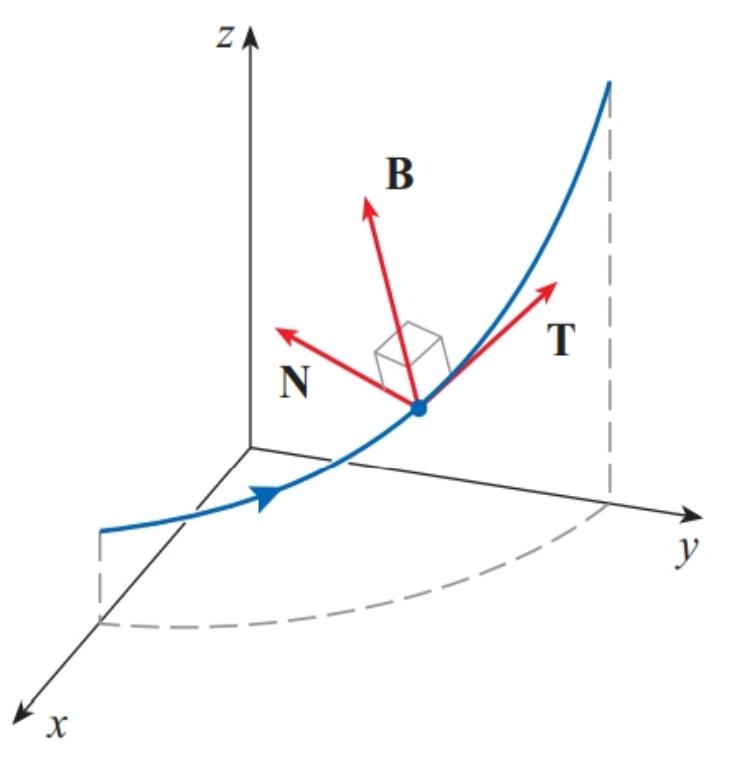
\includegraphics[scale=0.2]{figuras/normal-binormal.png}
\end{minipage}
Estes três vetores formam uma base ortonormal muito importante em geometria diferencial e no estudo de movimento de corpos, chamada de {\color{blue} Triedro de Frenet}.

\end{frame}

\begin{frame}[label=fun-vet]
\begin{exe}
Determine os vetores normal e binormal da hélice circular $$\vec{r}(t)=(\cos(t),\sin(t),t).$$

\end{exe}
\end{frame}

%\begin{frame}[label=fun-vet]
%\begin{casa}
%\begin{enumerate}
%\item Calcule a curvatura de uma reta.
%\item Calcule a curvatura de uma elipse $\frac{x^2}{a^2}+\frac{y^2}{b^2}=1$.
%\end{enumerate}
%\end{casa}
%
%
%\end{frame}

\subsection*{Movimento de partículas}
\begin{frame}[label=fun-vet]{Movimento: velocidade e aceleração}
	Suponha que uma partícula se mova de forma que seu vetor posição no instante $t$ seja $\vec{r}(t)$. Então vamos denotar por:
	\begin{itemize}
		\item $\vec{v}(t)=\vec{r}\,'(t)$ é o vetor \dt{velocidade da partícula} no instante $t$.
		\item $v(t)=\|\vec{v}(t)\|$ é a \dt{velocidade escalar} da partícula no instante $t$.
		\item $\vec{a}(t)=\vec{r}\,''(t)$ é o vetor \dt{aceleração} da partícula no instante $t$.
		\item $a(t)=\|\vec{a}(t)\|$ a aceleração escalar da partícula no instante $t$.
	\end{itemize}

\end{frame}


\begin{frame}[label=fun-vet]
Podemos mostrar que  a aceleração é dada por:
\[{\color{red}\vec{a}=v'\vec{T}+v^2\kappa \vec{N}. }\]
Com isso temos as seguintes conclusões:
\begin{itemize}
\item O vetor $\vec{B}$ não aparece, ou seja, a aceleração sempre está no plano determinado por $\vec{T}$ e $\vec{N}$, chamado {\color{blue} plano osculador}.


\item A componente tangencial da aceleração mede a taxa de variação do módulo da  velocidade, isto é, a mudança na velocidade escalar.

\item A componente normal é dada pelo quadrado da velocidade escalar e pela curvatura.
\end{itemize}

\begin{exe}
Um objeto de massa $m$ que se move em uma trajetória circular com velocidade angular constante $\omega$ tem vetor posição dado por $\vec{r}(t)=(\rho\cos (\omega t), \rho\sin (\omega t)).$ Determine a força que age sobre o objeto.
\end{exe}
\end{frame}


\subsection*{Fórmula para a curvatura}
\begin{frame}[label=fun-vet]
Usando a última equação, podemos deduzir a seguinte fórmula para a curvatura.
\begin{teo}
A curvatura de uma curva parametrizada suave $\vec{r}=\vec{r}(t)$ é dada por:
\[\kappa(t)=\frac{\|\vec{v}(t)\times \vec{a}(t)\|}{v^3(t)}=\frac{\|\vec{r}\,^\prime(t)\times \vec{r}\,^{\prime\prime}(t)\|}{\|\vec{r}\,^\prime(t)\|^3}.\]
\end{teo}

\begin{exe}
Determine a curvatura da cúbica retorcida $\vec{r}(t)=(t,t^2,t^3)$.
\end{exe}
\end{frame}


\begin{frame}[label=fun-vet]
	\begin{casa}
		\begin{enumerate}
		
	\item  Mostre que a curvatura de uma curva plana que tem equação cartesiana da forma $y=f(x)$ é dada por:
	\[\kappa(x)=\frac{|f''(x)|}{\left(1+[f'(x)]^2\right)^{3/2}}.\]
		
	\item Calcule a curvatura da parábola $y=x^2$ e determine o ponto onde a curvatura é máxima.
	
	\item Determine as componentes normal e tangencial da aceleração da partícula que se move segundo a trajetória $\vec{r}(t)=e^{-t}\,\vec{i}+e^t\,\vec{j}$.
	
	\item Uma partícula se move sobre a parábola $y=x^2$ da esquerda para a direita. Quando ela passa pelo ponto $(2,4)$, sua velocidade é $v=3$ m/s e $v'=7$ m/s$^2$. Ache o vetor velocidade e o vetor aceleração neste ponto.
	
	
%	\item Determine as componentes tangencial e normal do vetor aceleração da curava 
	%\[\vec{r}(t)=(t^2+1)\vec{i}+t^3\vec{j}, \ t\geq 0.\]
		

%\item Determine uma parametrização para a reta tangente à hélice $\vec{r}(t)=\left(2\cos t,\sin t, t\right)$ no ponto $P=(0,1,\pi/2)$.
%			
%			\item Determine o comprimento de arco da cardioide $r=2(1+\cos \theta)$.
%			
%			\item Determine os vetores velocidade e aceleração e a velocidade escalar da partícula cuja função posição é 
%			\[\vec{r}(t)=3\cos(t)\,\vec{i}+2\sin( t)\, \vec{j},  0\leq t\leq 2\pi.\]
%			Faça um esboço da trajetória e marque os vetores velocidade onde a velocidade escalar é mínima e máxima.
		\end{enumerate}
	\end{casa}
\end{frame}





\section{Funcões de Várias Variáveis}



\subsection*{Definição}
\begin{frame}[label=funcoes]
\frametitle{Funções de Várias Variáveis }
%\begin{scriptsize}

\uncover<1->{ Uma \dt{função real $f$ de $n$ variáveis} é uma relação que associa a cada n-upla $(x_1,\ldots,x_n)\in D\subset \R^n$ um único  número real $z=f(x_1,\ldots,x_n)$. O subconjunto $D$ de $\R^n$ é chamado \dt{domínio} da função $f$. Podemos denotar a função $f$ por
\[\begin{array}{ccl}
f:& D\subset\R^n & \longrightarrow \R\\
& (x_1,\ldots,x_n) & \longmapsto z=f(x_1,\ldots,x_n)
\end{array}\]
 }

\begin{center}
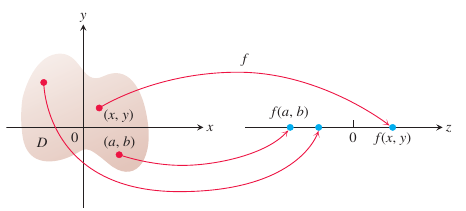
\includegraphics[scale=.7]{figuras/func.png}
\end{center}

%\end{scriptsize}
\end{frame}

\begin{frame}[label=funcoes]

\begin{exe} \begin{enumerate}
\item A função $V(r,h)=\pi r^2h$, $r,h>0$ é uma função de duas variáveis que  fornece o volume de um cilindro circular reto de raio da base $r$ e altura $h$.

 \item A função $z=f(x,y)=\frac{1}{x-y}$ é uma função de duas variáveis cujo domínio são todos os pontos $(x,y)\in \R^2$ tais que $x\neq y$.
 
 \item A função $\dps f(x,y,z)=\frac{1}{(x^2+y^2+z^2)^{3/2}}$ é uma função de três variáveis cujo domínio são todos os pontos $(x,y,z)\in \R^3$ tais que $x^2+y^2+z^2\neq 0$, ou seja, $\R^3\setminus\{0\}$.
 \end{enumerate}
 \end{exe}
 
\end{frame}


\subsection*{Gráfico de função de duas variáveis}
\begin{frame}[label=funcoes]{Gráfico de uma função de duas variáveis}
%\begin{scriptsize}

O \dt{gráfico de uma função} $f:D\subset \R^2\to \R$, denotado por $G_f$, é o subconjunto do $\R^{3}$ formado por todos os pontos  da forma $(x,y,f(x,y))$, isto é,
\[G_f:=\{(x,y,z)\in \R^{3};\ z=f(x,y),\ (x,y)\in \R^2\}\] 

\begin{center}
	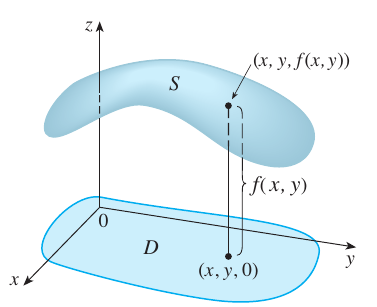
\includegraphics[scale=0.5]{figuras/grafico-f.png}
\end{center}



%\uncover<1->{\begin{exe} A temperatura em cada ponto $(x,y)$ de uma placa de metal plana é dada, em graus, pela função $T(x,y)=9x^2+4y^2$.
%\begin{enumerate}[a)]
%\item Encontre a temperatura no ponto $(1,2)$.
%\item Encontre a equação da curva ao longo da qual a temperatura tem um valor constante e igual a 36 graus.
%\item Esboce a curva do item anterior.
%\end{enumerate}
%\end{exe}}

%\end{scriptsize}
\end{frame}


\begin{frame}[label=funcoes]
	
	\begin{block}{Temperatura abaixo da superfície da Terra}
 A temperatura ${\color{red}w}$ abaixo da superfície da Terra é uma função da profundidade $x$ abaixo da superfície e da época do ano $t$. Se medirmos ${\color{blue}x}$ em pés e ${\color{blue}t}$ como o número de dias decorridos a partir da data esperada da maior temperatura anual da superfície, podemos modelar a variação da temperatura com a função
 \[{\color{red}w}=\cos(1.7\times 10^{-2}{\color{blue}t}-0.2 {\color{blue}x})e^{-0.2 {\color{blue}x}}\]
	\end{block}
	
	

\begin{center}
	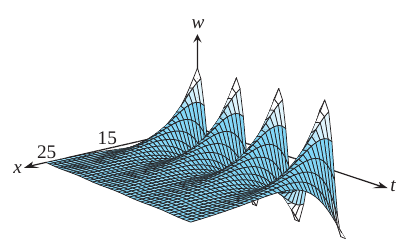
\includegraphics[scale=0.5]{figuras/grafico-2.png}
\end{center}
	
\end{frame}

\begin{frame}[label=funcoes]
\begin{exe}
	Esboce o gráfico da função  $f(x,y)=6-3x-2y$.
\end{exe}
\end{frame}

\begin{frame}[label=funcoes, fragile=singleslide]
\begin{block}{ }
\begin{scriptsize}
\begin{pyverbatim}
import matplotlib.pyplot as plt
import numpy as np

def f(x, y):
    return 6-3*x-2*y

x =y=np.linspace(-5,5, 25)

X,Y=np.meshgrid(x, y)
Z = f(X, Y)

fig=plt.figure()
ax=plt.axes(projection='3d')

ax.set_xlabel('x')
ax.set_ylabel('y')
ax.set_zlabel('z')
ax.plot_surface(X, Y, Z,cmap='viridis')

plt.show()
\end{pyverbatim}
\end{scriptsize}
\end{block}



\end{frame}

\begin{frame}[label=funcoes,fragile=singleslide]
\begin{pycode}
import matplotlib.pyplot as plt
import numpy as np

def f(x, y):
    return 6-3*x-2*y

x =y= np.linspace(-5,5, 25)

X, Y = np.meshgrid(x, y)
Z = f(X, Y)

fig = plt.figure()
ax = plt.axes(projection='3d')
ax.view_init(elev=30, azim=30, roll=0)

ax.set_xlabel('x')
ax.set_ylabel('y')
ax.set_zlabel('z')
ax.plot_surface(X, Y, Z,cmap='viridis')


plt.savefig('figuras/grafico1.png',transparent=False,dpi=400)
\end{pycode}

\begin{center}
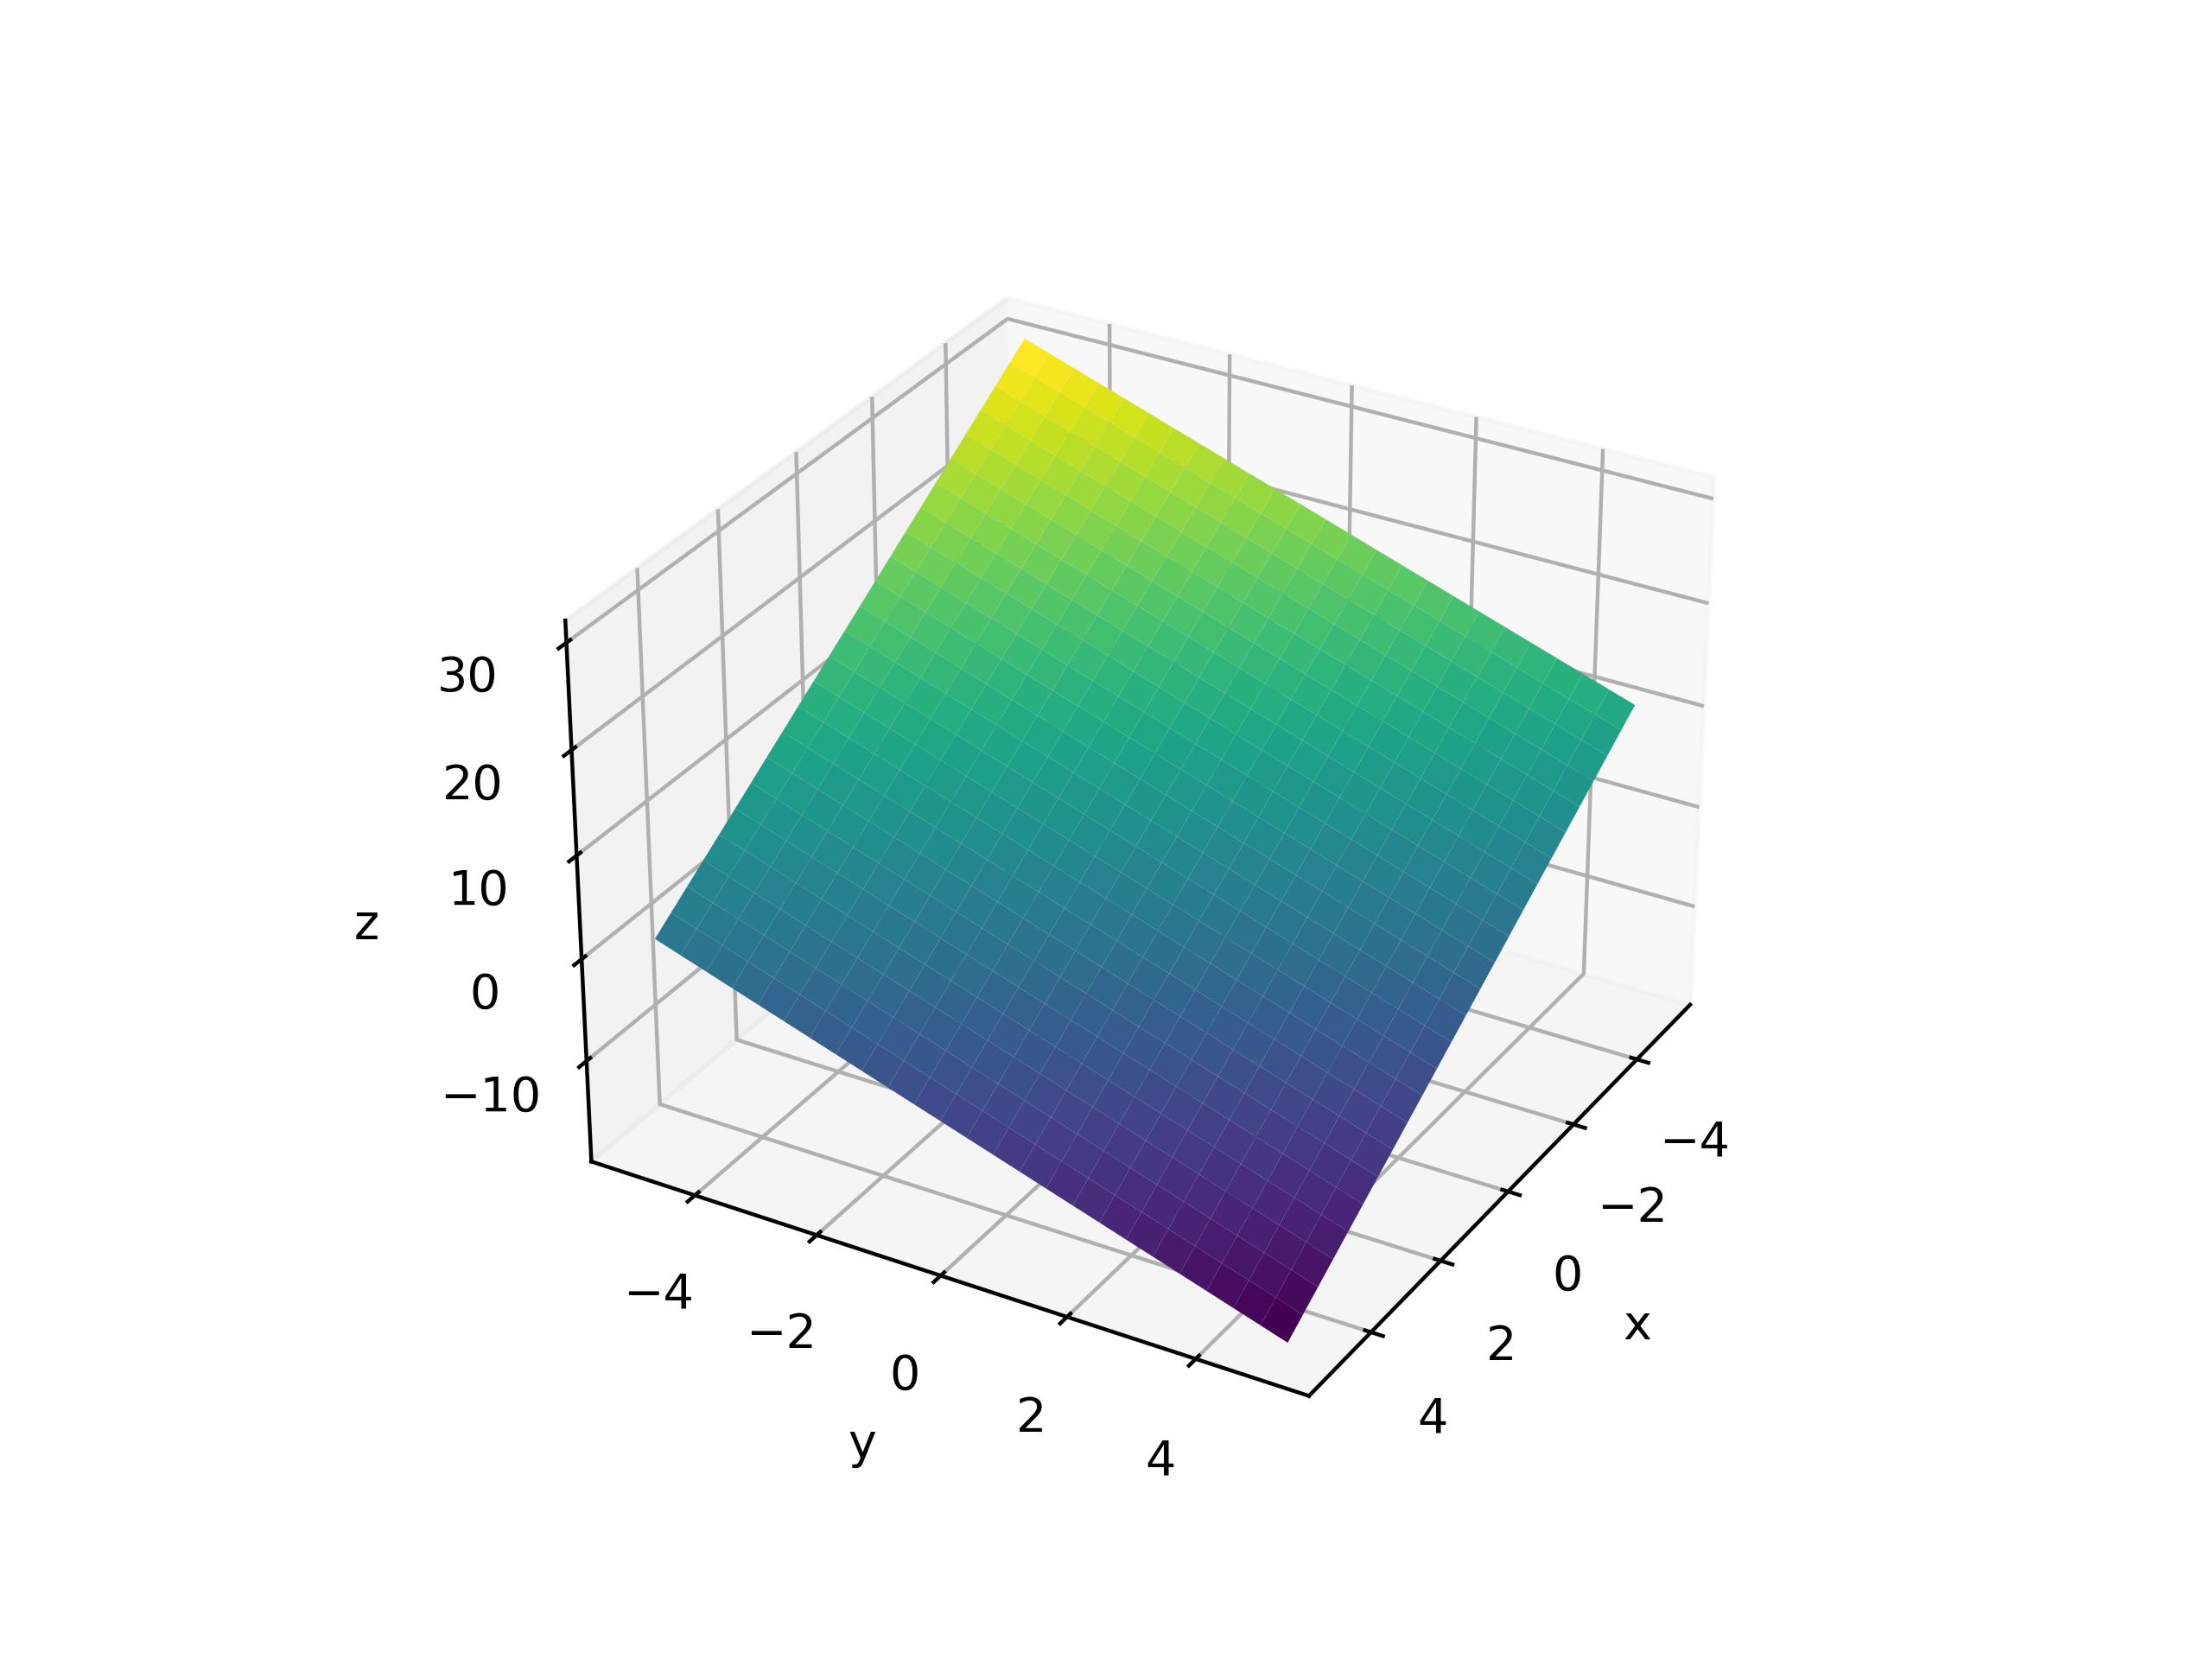
\includegraphics[scale=0.7]{figuras/grafico1.png}
\end{center}
\end{frame}


\subsection*{Curvas de Nível}

\begin{frame}[label=funcoes]
\frametitle{Curvas e Superfícies de Nível }
%\begin{scriptsize}

Uma curva ao longo da qual uma função $z=f(x,y)$ tem valor constante é denominada \dt{curva de nível} da função $f$.

\begin{center}
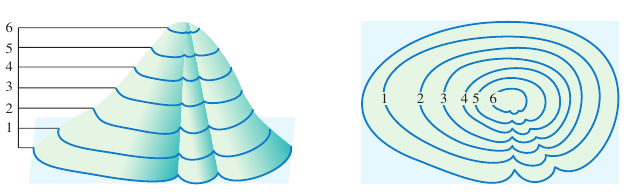
\includegraphics[scale=0.5]{figuras/nivel1.png}
\end{center}

 Quando a função $f$ representa a temperatura, as curvas de nível de $f$ são chamadas \dt{isotermas}. Se $f$ representa o potencial elétrico, as curvas de nível de $f$ são ditas \dt{curvas equipotenciais}. A equação da curva de nível ao longo da qual a função assume valor constante $k$ é
$$f(x,y)=k.$$
Se $S$ é a superfície do gráfico de uma função $f$, um conjunto de curvas de nível de uma função $f$ é dito \dt{um mapa de contorno da superfície $S$}.



%\end{scriptsize}
\end{frame}

\begin{frame}[label=funcoes]
\only<1>{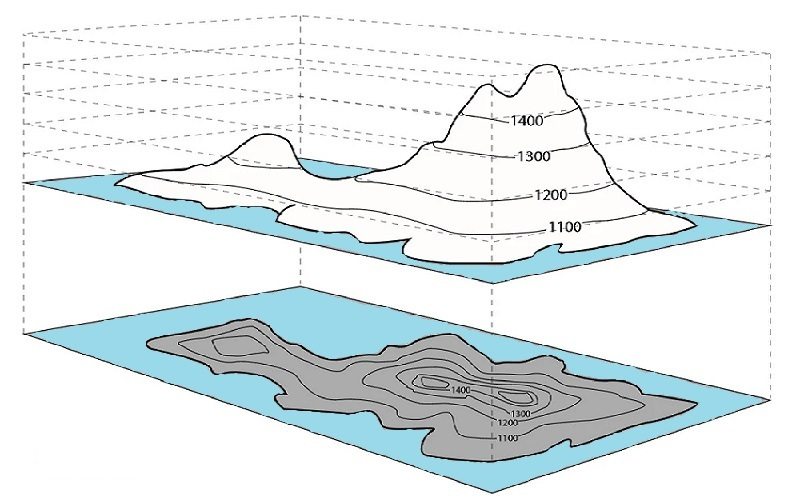
\includegraphics[scale=0.6]{figuras/nivel3.jpg}}
\end{frame}

\begin{frame}[label=funcoes]
\begin{exe}
		A temperatura em cada ponto $(x,y)$ de uma placa de metal plana é dada, em graus, pela função $T(x,y)=9x^2+4y^2$. Faça uma mapa de contorno das isotermas.
\end{exe}
\end{frame}



\begin{frame}[label=funcoes]
\begin{center}

\only<1>{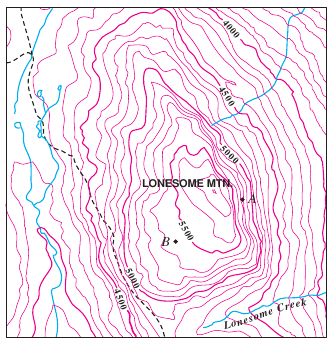
\includegraphics[scale=0.9]{figuras/nivel2.png}

Mapa topográfico de uma região montanhosa.
}
\only<2>{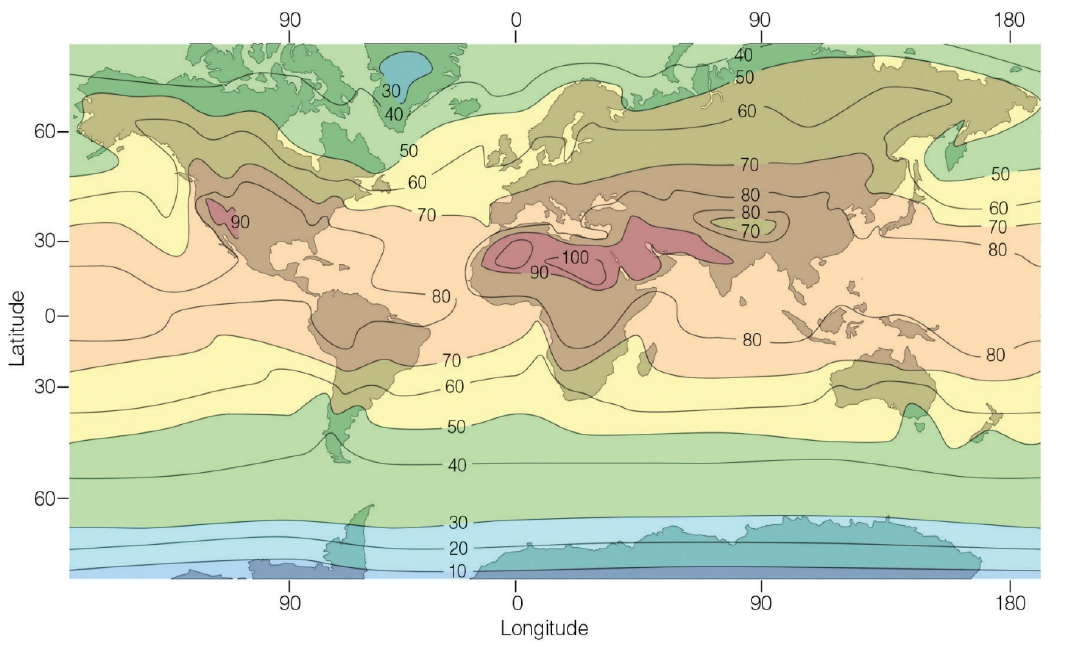
\includegraphics[scale=0.4]{figuras/nivel3.png}

Temperatura média do ar ao nível do mar no mês de julho em Fahrenheit}
\only<3>{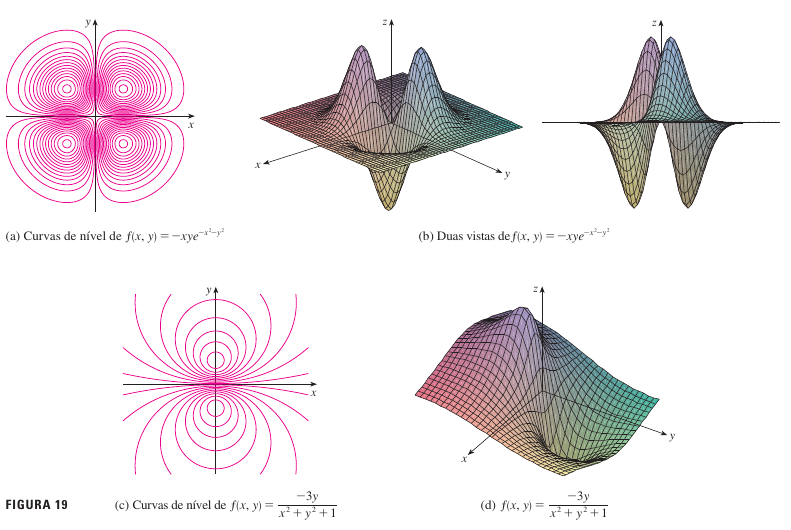
\includegraphics[scale=0.6]{figuras/nivel4.png}}
\only<4>{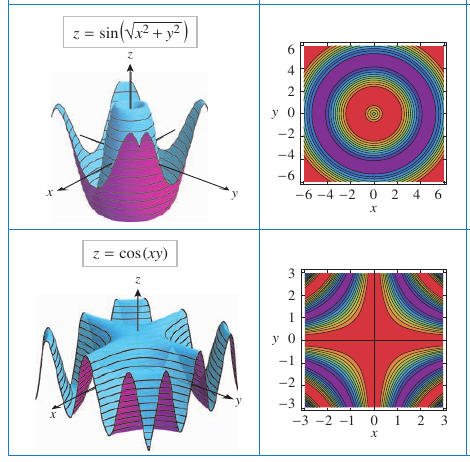
\includegraphics[scale=0.6]{figuras/nivel5.png}

Degradê de cores para indicar os níveis. Varia do roxo para o vermelho na ordem crescente.
}
\only<5>{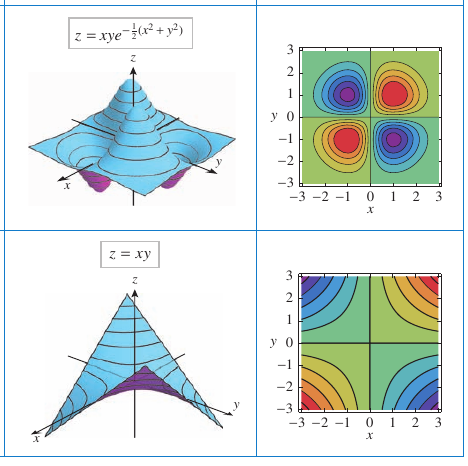
\includegraphics[scale=0.7]{figuras/nivel6.png}}
\end{center}
\end{frame}




\subsection*{Superfícies de Nível}
\begin{frame}[label=funcoes]
\frametitle{Superfícies de Nível}
%\begin{scriptsize}
\uncover<1->{ No caso de funções de três variáveis, um conjunto no qual uma função $f(x,y,z)$ tem valor constante é dita \dt{uma superfície de nível} da função $f$.

\begin{exe} Descreva as superfícies de nível da função $f(x,y,z)=x^2+y^2+z^2$.
\end{exe}}

\begin{center}
	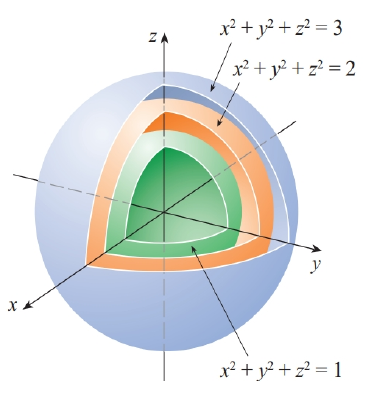
\includegraphics[scale=0.5]{figuras/nivel-superfice.png}
\end{center}

%\end{scriptsize}
\end{frame}


\begin{frame}[label=funcoes]
\begin{casa}
\begin{enumerate}
\item Esboce a região de domínio da função 
\[f(x,y)=x\log(y^2-x)\]
\item Determine o domínio e esboce o gráfico da função  $f(x,y)=\sqrt{9-x^2-y^2}$.

\item Faça um mapa de contorno da função $f(x,y)=4-x^2-y$ para os níveis $5,4,3,2,1,0,-1$ e faça um esboço do gráfico.

\item Descreva as superfícies de nível da função $f(x,y,z)=z-x^2-y^2$.
\end{enumerate}
\end{casa}
\end{frame}

\section{Limite e Continuidade}

%
%\begin{frame}
%	\frametitle{Noções de Topologia no $\R^2$ }
%	\begin{scriptsize}
%		
%		\uncover<1->{Dados $r>0$ e $P_0=(x_0,y_0)\in \R^2$ o conjunto
%			$$\{(x,y)\in \R^2; (x-x_0)^2+(y-y_0)^2<r\}$$
%			denomina-se \dt{bola aberta} de centro $(x_0,y_0)$ e raio $r>0$ e é denotado por $B_r(P_0)$.
%			\bigskip
%			
%			Seja $U$ um subconjunto de $\R^2$. Dizemos que um ponto $(x_0,y_0)\in U$ é um \dt{ponto interior} de $U$ se existir uma bola aberta de centro em $(x_0,y_0)$ interiamente contida  em $U$.  
%			
%			\begin{exe}Seja $U=\{(x,y)\in\R^2;\ x\geq 0, y\geq 0\}$\begin{enumerate}[a]
%					\item O ponto $(1,2)$ é ponto interior a $U$.
%					\item Todo ponto tal que $(x,y)$ tal que $x>0$ e $y>0$ é ponto interiro a $U$.
%					\item $(0,1)$ não é ponto interior a $U$
%				\end{enumerate}
%			\end{exe}
%			
%		}
%		
%	\end{scriptsize}
%\end{frame}
%
%
%\begin{frame}
%	\frametitle{ }
%	\begin{scriptsize}
%		
%		\uncover<1->{Dado $U\subset\R^2$, dizemos que um ponto $(x_0,y_0)$ é \dt{ponto de fronteira} de $U$ se para toda bola aberta de centro em $(x_0,y_0)$ contém pontos de $U$ e pontos em $\R^2\setminus U$. O conjunto de todos os pontos de fronteira de $U$ é denominado \dt{fronteira de $U$} e denotado por $\partial U$. 
%			\bigskip
%			
%			Um conjunto $U$ é dito $aberto$ quando todos os seus pontos são pontos interiores. Um conjunto é dito \dt{fechado} contém todos os seus pontos de fronteira..
%			\bigskip
%			
%			Um ponto $(x_0,y_0)\in U$ é dito \dt{ponto de acumulação } de $U$ quando toda bola $B_r(x_0,y_0)$ contém pelo menos um ponto  de $U$ diferente de $U$.
%		}
%		
%		\uncover<2->{\begin{exe} 
%				\begin{enumerate}[a)]
%					\item Toda bola aberta é um conjunto aberto.
%					\item $\R^2$ e o conjunto vazio são conjuntos aberto e fechado ao mesmo tempo.
%					\item $U=\{(x,y)\in \R^2;\ x\geq 0 \mbox{ e } y>0 \}$ não é aberto e nem fechado.
%					\item $(0,0)$ é ponto de acumulação de $U=\{\left(\frac{1}{n},0\right);\ n\in\mathbb{N}\}$.
%				\end{enumerate}
%		\end{exe}}
%		
%	\end{scriptsize}
%\end{frame}

\subsection*{Limites}
\begin{frame}[label=limites]{Limites}
Seja $f:D\subset\R^2\to \R$ uma função cujo domínio contém pontos arbitrariamente próximos de {\color{blue}$(a,b)$}. Usamos a notação 
	\[\lim_{(x,y)\to {\color{blue}(a,b)}}f(x,y)={\color{red}L},\]
	para indicar que os valores de $f(x,y)$ se aproximam do número {\color{red}$L$} quando o ponto $(x,y)$ se aproxima do ponto {\color{blue}$(a,b)$} ao longo de qualquer cominho contido no domínio da função $f$.
\end{frame}

\subsection*{definição}
\begin{frame}[label=limites]
	\frametitle{Limite}
%	\begin{scriptsize}
		
		\begin{defin} Seja $f:D\subset\R^2\to \R$ uma função cujo domínio contém pontos arbitrariamente próximos de {\color{blue}$(a,b)$}. Dizemos que {\color{blue} o limite de $f(x,y)$ quando $(x,y)$ tende a $(a,b)$} é o número {\color{blue}$L$}, e escrevemos
				\[\lim_{(x,y)\to {\color{blue}(a,b)}}f(x,y)={\color{red}L},\]
				quando para cada $\varepsilon>0$, existe $\delta>0$ tal que se $\|(x,y)-{\color{blue}(a,b)}\|<\delta$, então $|f(x,y)-{\color{red}L}|<\varepsilon$.
		\end{defin} 

\end{frame}

\begin{frame}[label=limites]
	\begin{center}
		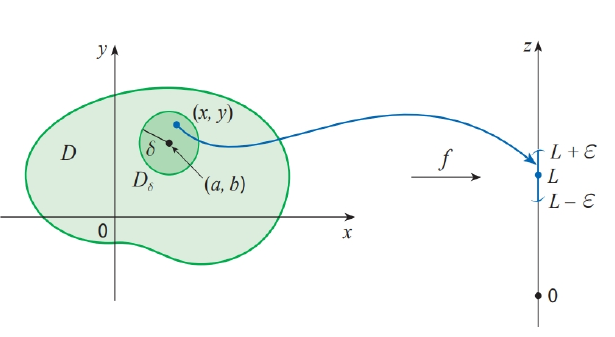
\includegraphics[scale=0.5]{figuras/limite1.png}

		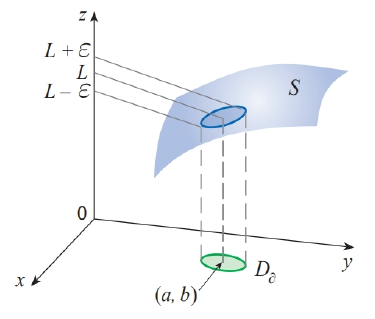
\includegraphics[scale=0.5]{figuras/limite2.png}

	\end{center}
\end{frame}


\begin{frame}[label=limites]
		Todas as propriedades de limites de funções  de uma variável se estendem às funções de várias variáveis. Por exemplo, o limite da soma, diferença, produto ou quociente é a soma, diferença, produto ou quociente dos limites, respectivamente, contanto que esses limites existam e que os denominadores não se anulem.
		\begin{exe} Calcule 
			$\dps\lim_{(x,,y)\to(-1,2)}\left(2x^2y-\frac{3y^2}{x+y}\right).$
	\end{exe}
\end{frame}


\begin{frame}[label=limites]{Mostrando que um limite não existe}

Quando o limite de uma função existe em um ponto, então o limite tem que ser o mesmo ao longo de todos os caminhos que se aproximam do ponto. 
\smallskip 

No plano podemos nos aproximar de um ponto {\color{blue}$(a,b)$} por {\color{red} um número infinito de caminhos}, assim se existem dois caminhos diferentes tais que $f(x,y)$ tende a valores distintos, então o limite não existe.


\begin{center}
	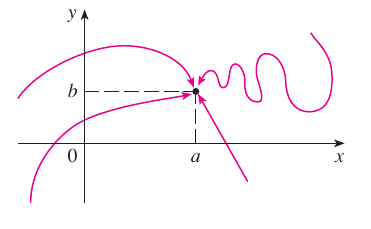
\includegraphics[scale=0.5]{figuras/lim-caminhos.png}
\end{center}

		
\end{frame}

\subsection*{Não existência de limite}
\begin{frame}[label=limites]
	\begin{exe} Mostre que o seguinte limite não existe
		\[\lim_{(x,y)\to(0,0)}\frac{x^2-y^2}{x^2+y^2}.\]
	\end{exe}  

	\begin{center}
		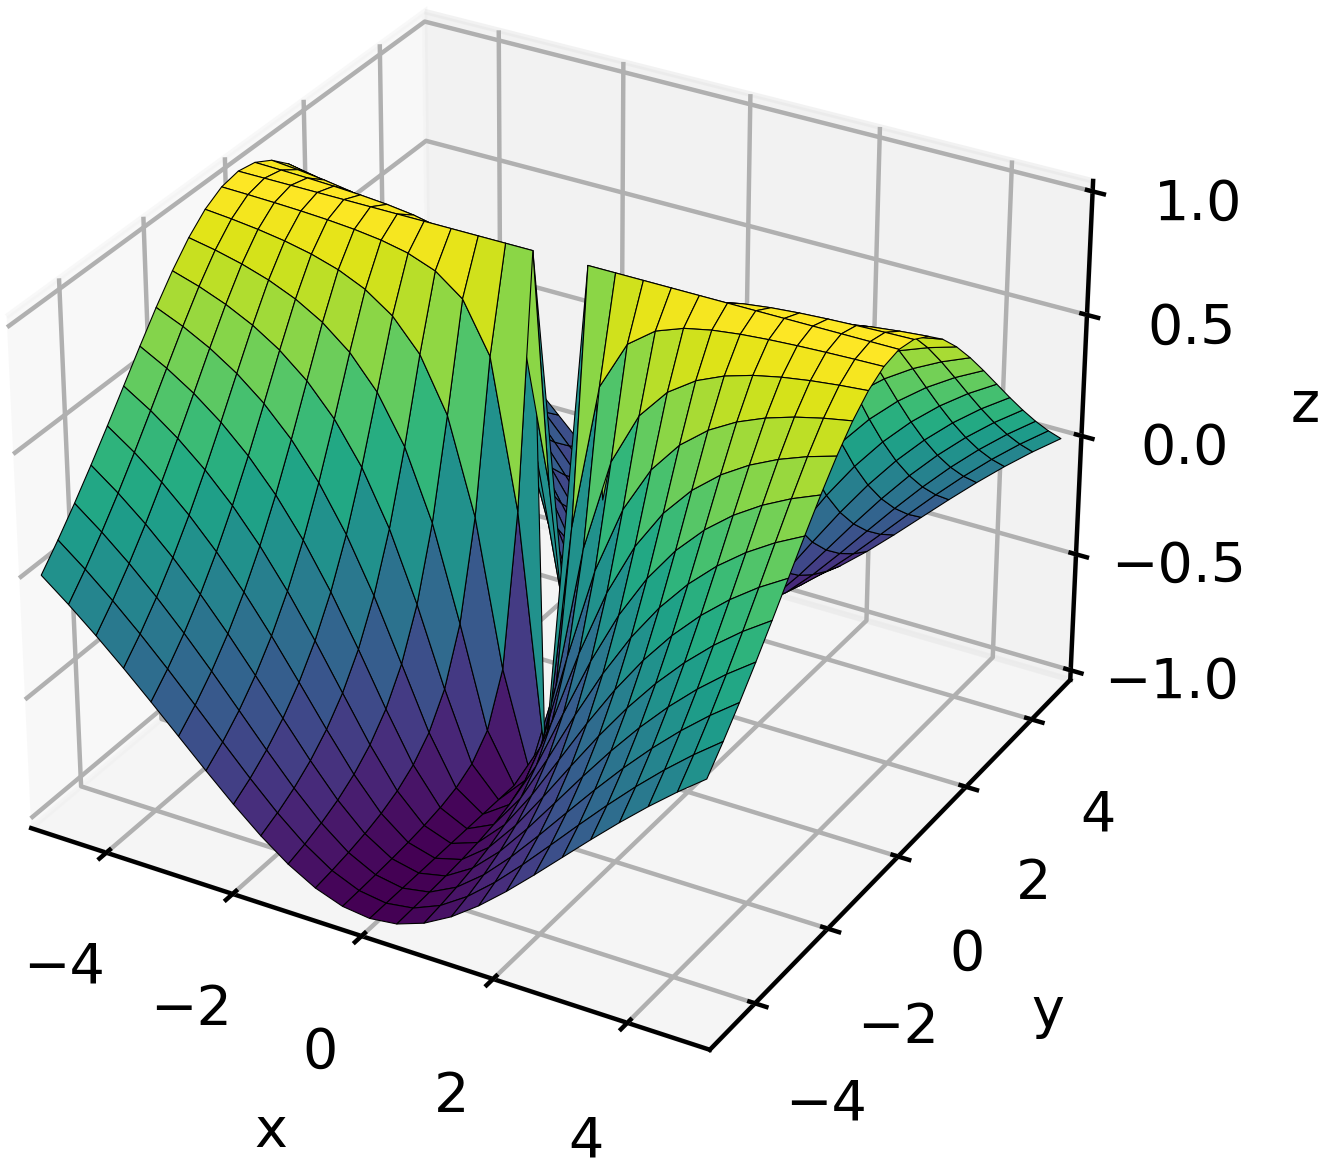
\includegraphics[scale=0.7]{figuras/lim1.png}
	\end{center}

\end{frame}

\begin{frame}[label=limites]
	\begin{exe}
		Mostre que o seguinte limite não existe
		\[\lim_{(x,y)\to(0,0)}\frac{xy}{x^2+y^2}\]
	\end{exe}

	\begin{center}
	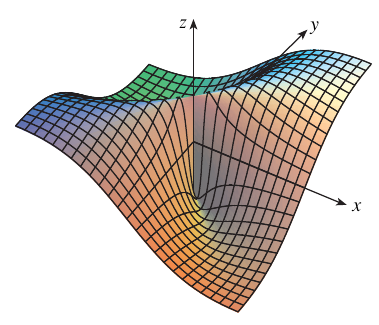
\includegraphics[scale=0.7]{figuras/lim2.png}
\end{center}
\end{frame}

\begin{frame}[label=limites]
	\begin{exe}
		Mostre que o seguinte limite existe
		\[\lim_{(x,y)\to(0,0)}\frac{2x^2y}{x^2+y^2}\]
	\end{exe}
	\begin{center}
	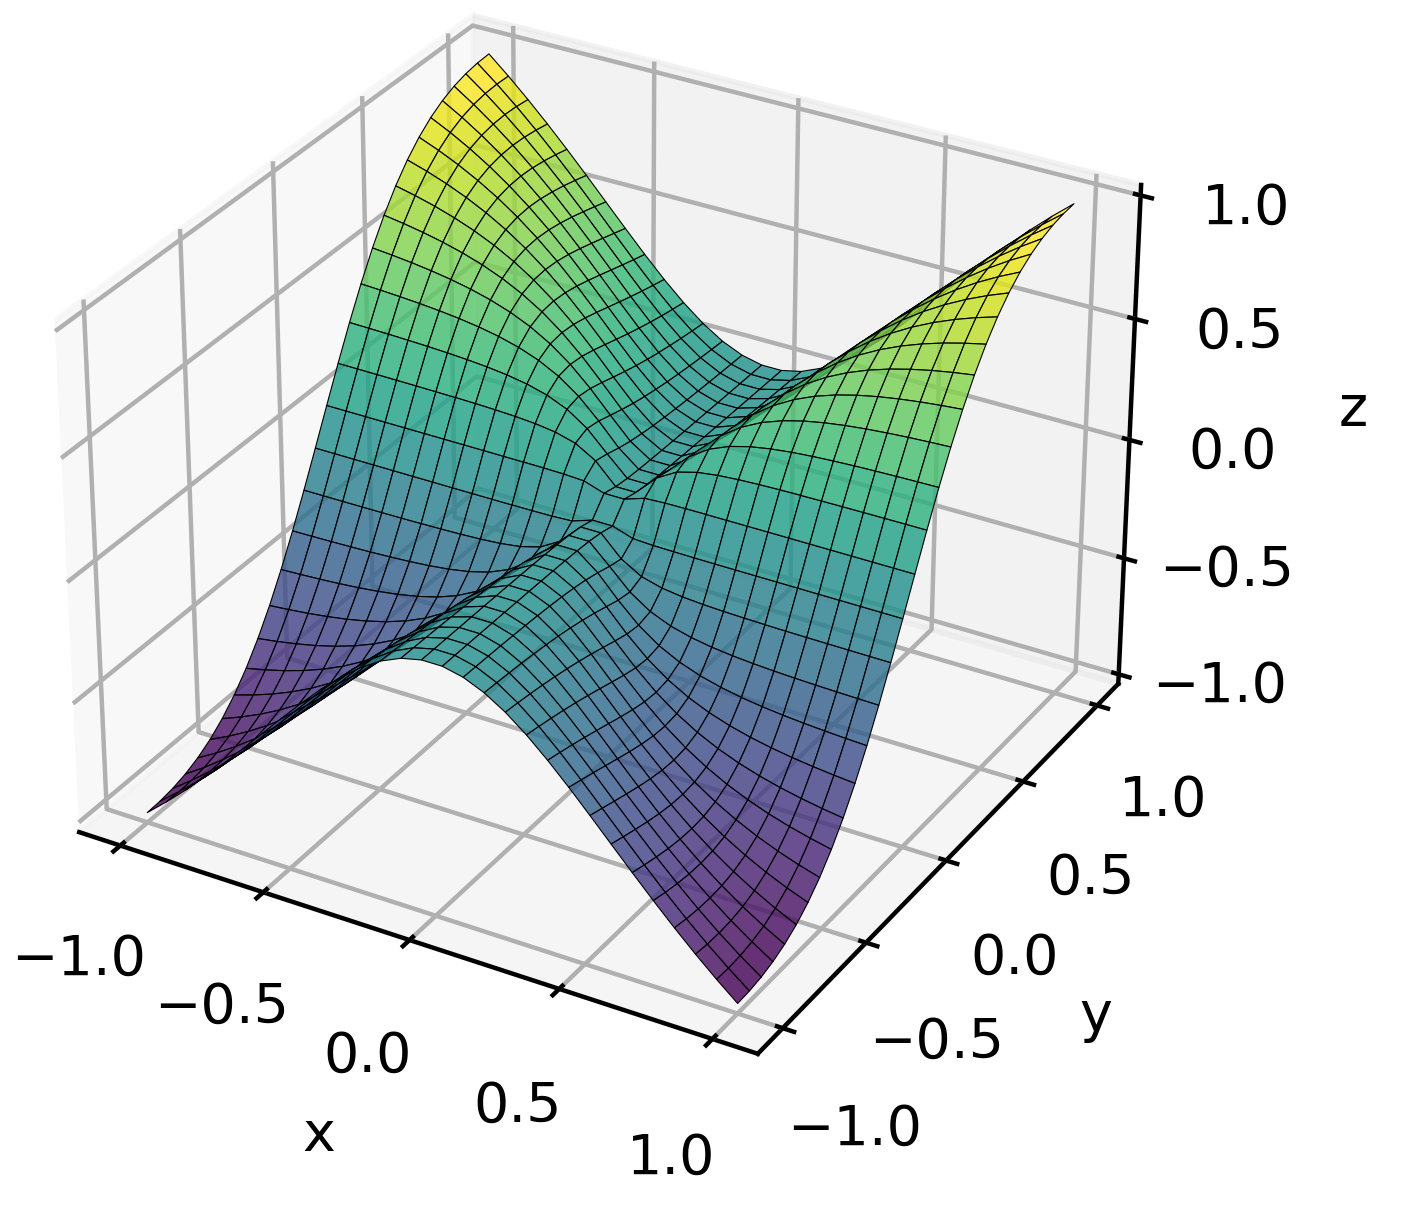
\includegraphics[scale=0.7]{figuras/lim3.png}
\end{center}
\end{frame}

\subsection*{Continuidade}
\begin{frame}[label=limites]
	\frametitle{Continuidade }

		
		\uncover<1->{\begin{defin} Sejam $f$ uma função real de duas variáveis e $(a,b)$ um ponto do domínio de $f$. Dizemos que $f$ é \dt{contínua} em $\pz$ se 
				$$\lim_{(x,y)\to\pz}f(x,y)=f\pz.$$
				Dizemos que $f$ é contínua em $D$ se $f$ é contínua em todos os pontos de $D$.
			\end{defin} 
		 }
		

\end{frame}


\begin{frame}[label=limites]
	
\begin{exe} \begin{enumerate}[a]
		\item Funções racionais são contínuas em todos os pontos de seu domínio.
		
		
		\item  A função $\arctan\left(\frac{y}{x}\right)$ é contínua em todo o seu domínio pois a composta de funções contínuas também é contínua.
	\end{enumerate}
\end{exe}

\begin{center}
	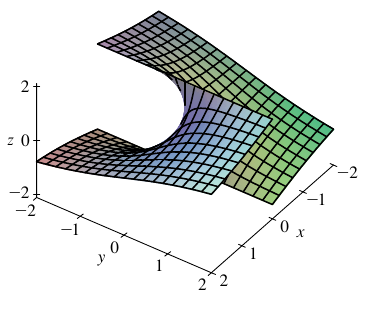
\includegraphics[scale=0.6]{figuras/cont1.png}
\end{center}
\end{frame}



\begin{frame}[label=limites]
	\frametitle{ }
	
		\uncover<1->{\begin{exe} Determine os pontos de continuidade de \begin{enumerate}[a]
					
					\item $f(x,y)=\left\{\begin{array}{ll}
						\dps\frac{2x^2y}{x^2+y^2}, &(x,y)\neq (0,0)\\
						\\
						0, & (x,y)=(0,0)\\
					\end{array}\right.$
					
					\item   $f(x,y)=\left\{\begin{array}{ll}
						\dps\frac{xy}{x^2+y^2}, &(x,y)\neq (0,0)\\
						\\
						0, & (x,y)=(0,0)\\
					\end{array}\right.$
				\end{enumerate}
		\end{exe} }
		
		\uncover<1->{Analogamente podemos generalizar estes resultados para funções de mais de duas variáveis quaisquer.}
		
\end{frame}

\begin{frame}[label=limites]
	\begin{casa}
		\begin{enumerate}
			\item Decida sobre a existência do seguinte limite $\dps\lim_{(x,y)\to(0,0)}\frac{x^2y}{x^4+y^2}$.
			
			\item Determine os pontos de continuidade da função
			\[f(x,y)=\begin{cases}
\frac{xy}{x^2+xy+y^2}, & (x,y)\neq (0,0),\\
0, & (x,y=(0,0).
			\end{cases}\]

\item Revise a definição de derivada de função de uma variável $y=f(x)$.
		\end{enumerate}
	\end{casa}
\end{frame}





\section{Derivadas Parciais}

\subsection*{Motivação}
\begin{frame}[label=der-parciais]{Derivadas Parciais}
Suponha que a distribuição de temperaturas em uma placa quadrada é descrita pela função
\[f({\color{red}x},{\color{blue}y})=100-{\color{red}x^2}-{\color{blue}y^2}, \text{ com } -5\sqrt{2}\leq {\color{red}x},{\color{blue}y}\leq 5\sqrt{2},\]
onde a temperatura é medida em $^\circ C$ e o comprimento em metros.




\begin{center}
 \begin{minipage}{0.5\textwidth}
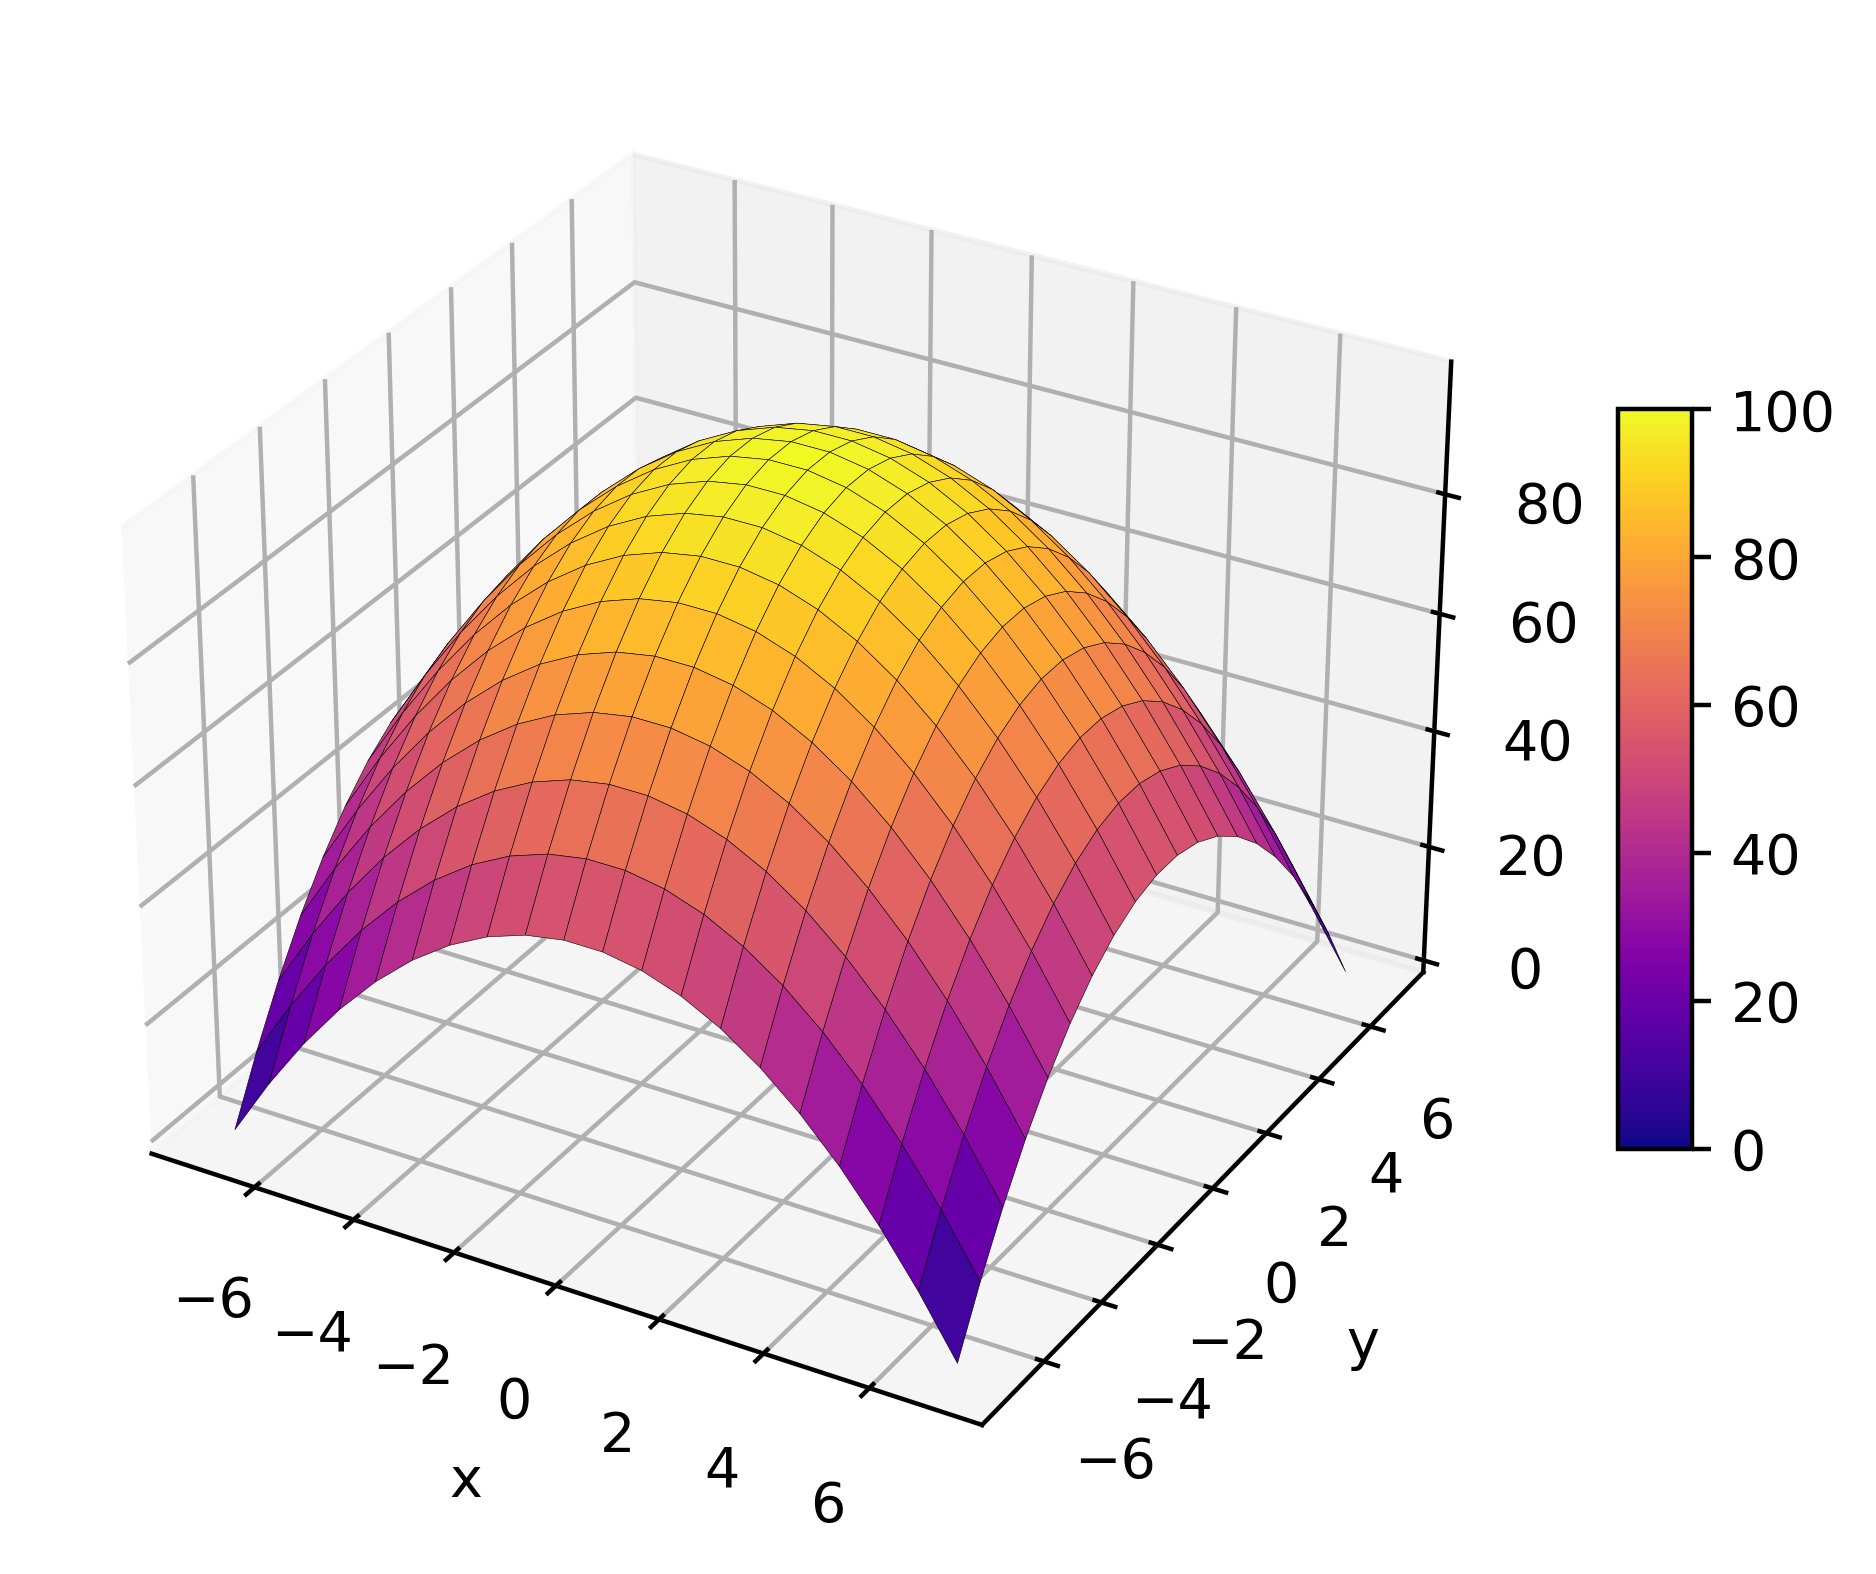
\includegraphics[scale=0.5]{figuras/der-parc2-1.png}
	 \end{minipage}
\begin{minipage}{0.4\textwidth}
	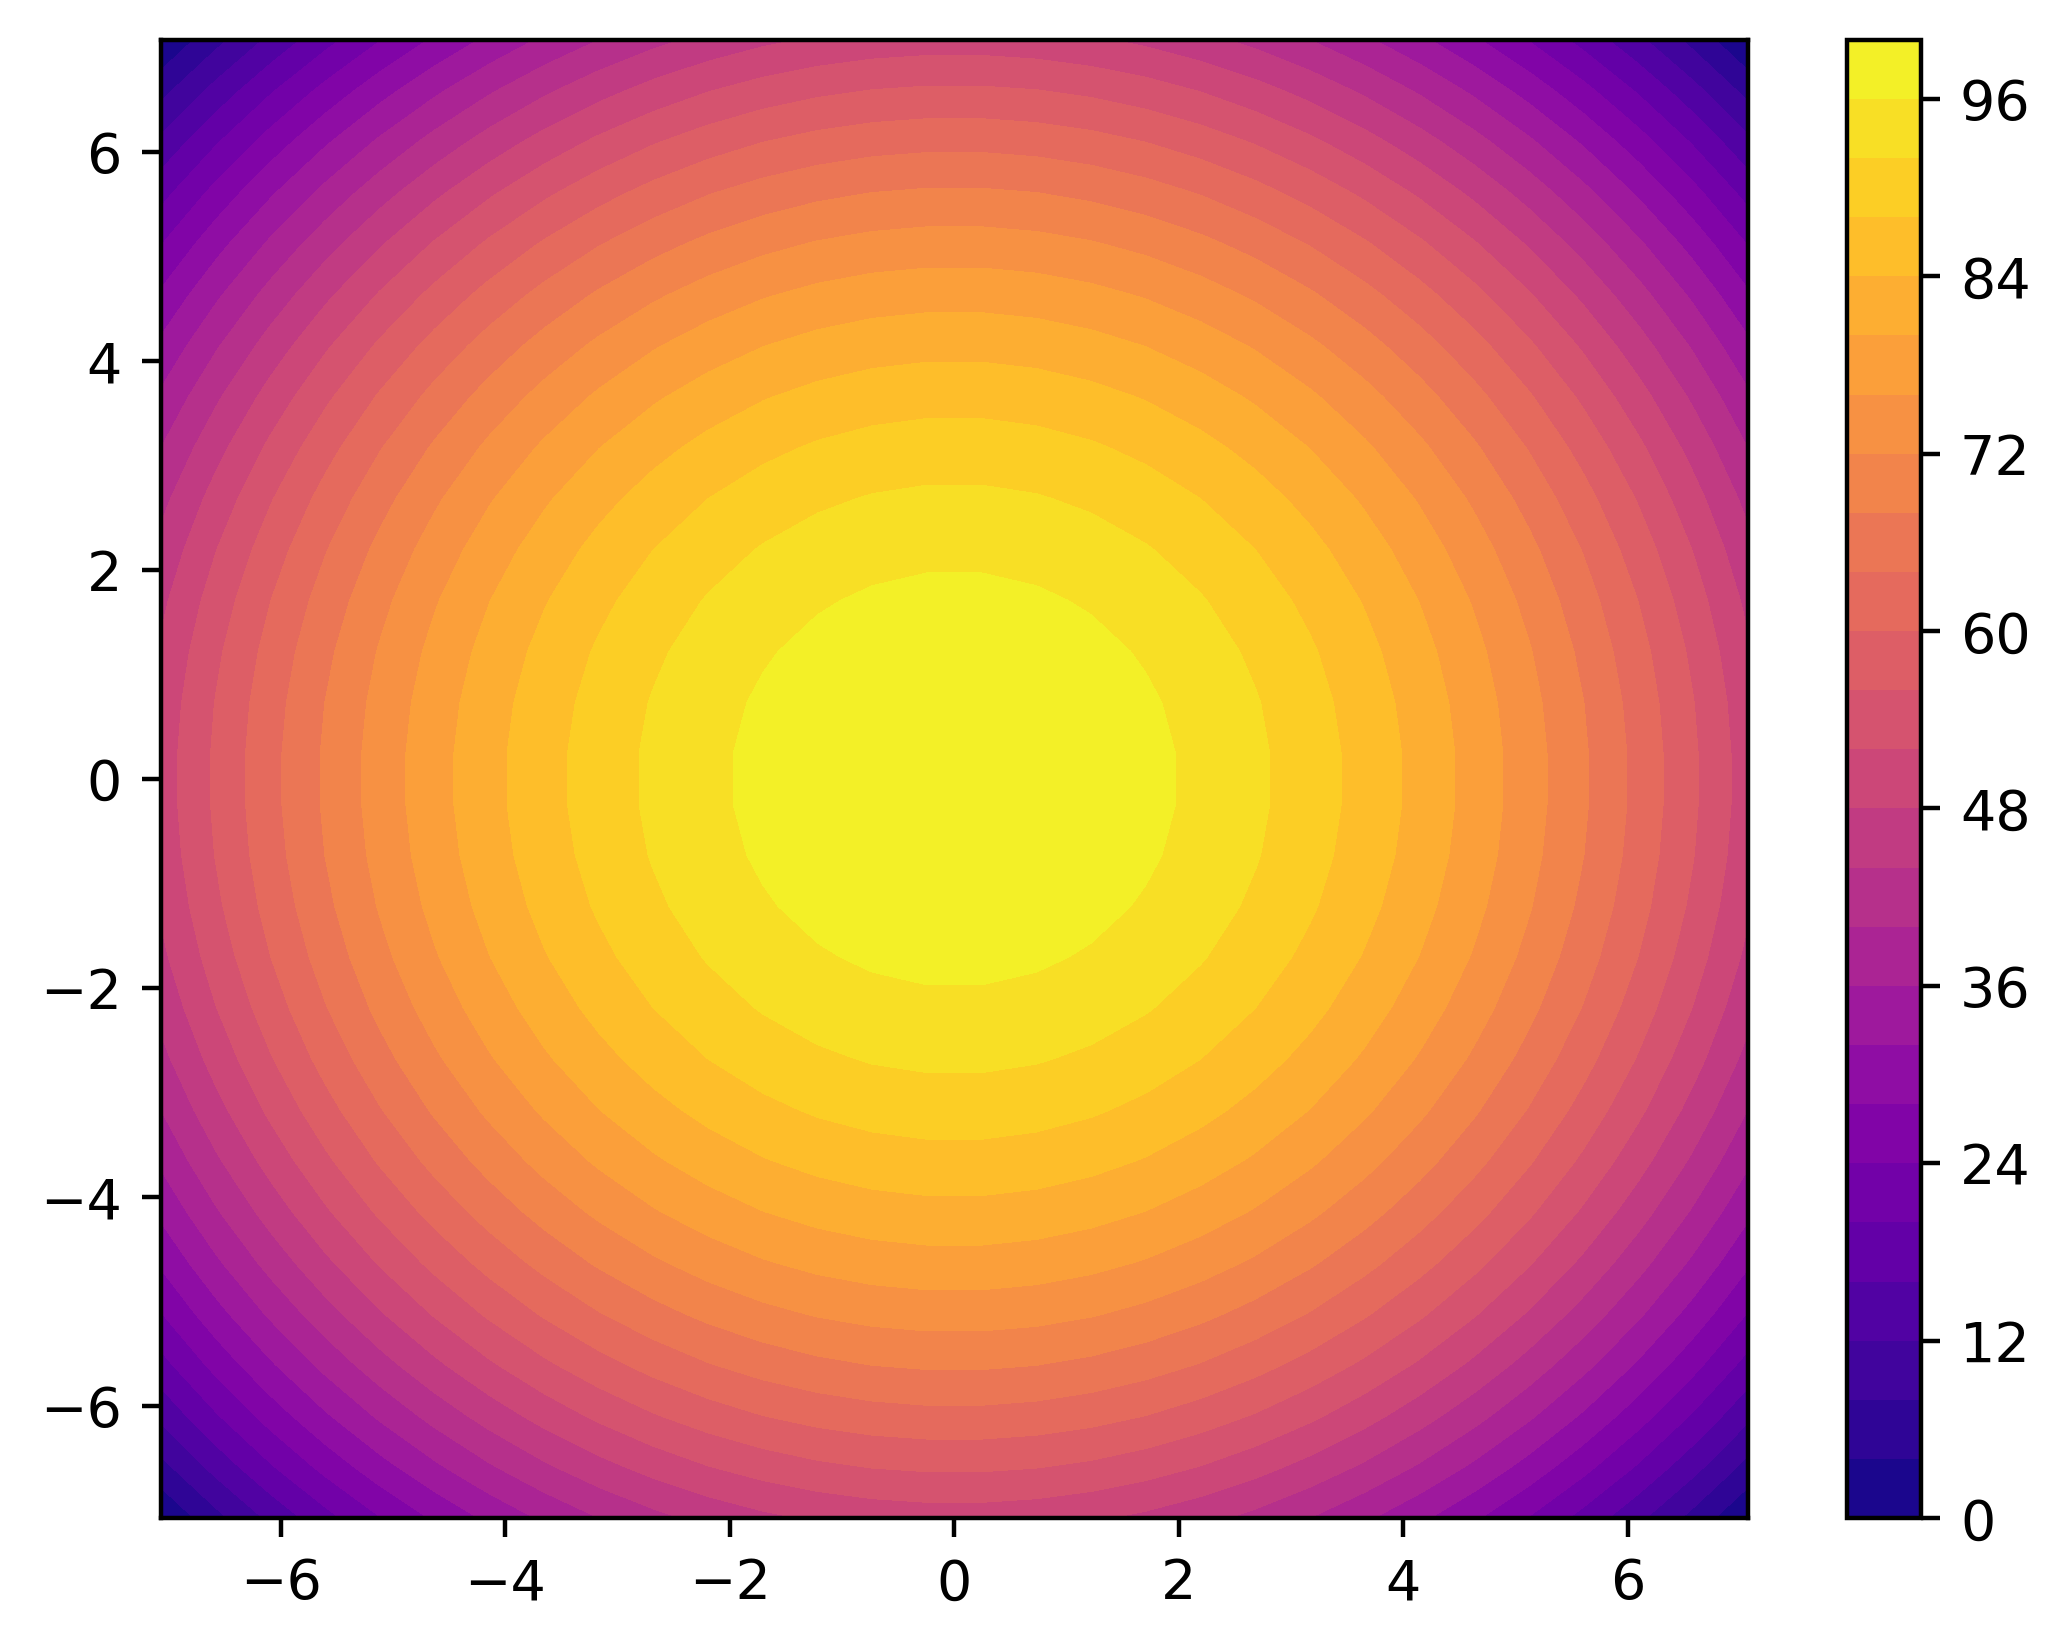
\includegraphics[scale=0.4]{figuras/der-parc2-1-nivel.png}
\end{minipage}
\end{center}


\end{frame}

%\begin{frame}[label=der-parciais]{Derivadas Parciais}
%Considere um paralelepípedo reto de altura {\color{blue}$y$} e base quadrada de lado {\color{red}$x$}.
%
%\begin{center}
%\begin{tikzpicture}
%\node at (0,0)
%{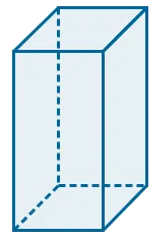
\includegraphics[scale=1]{figuras/paralelepidedo.png}};
%\node[color=red] at (-.2,-1.2) {$x$};
%\node[color=red] at (.7,-.8) {$x$};
%\node[color=blue] at (.8,.2) {$y$};
%\end{tikzpicture}
%\end{center}
%
%
% O volume deste paralelepípedo é dado pela função 
% \begin{minipage}{0.5\textwidth}
%\[V({\color{red}x},{\color{blue}y})={\color{red}x^2}{\color{blue}y}, \text{ com } {\color{red}x},{\color{blue}y}\geq 0.\]
% \end{minipage}
%\begin{minipage}{0.4\textwidth}
%\begin{center}
%	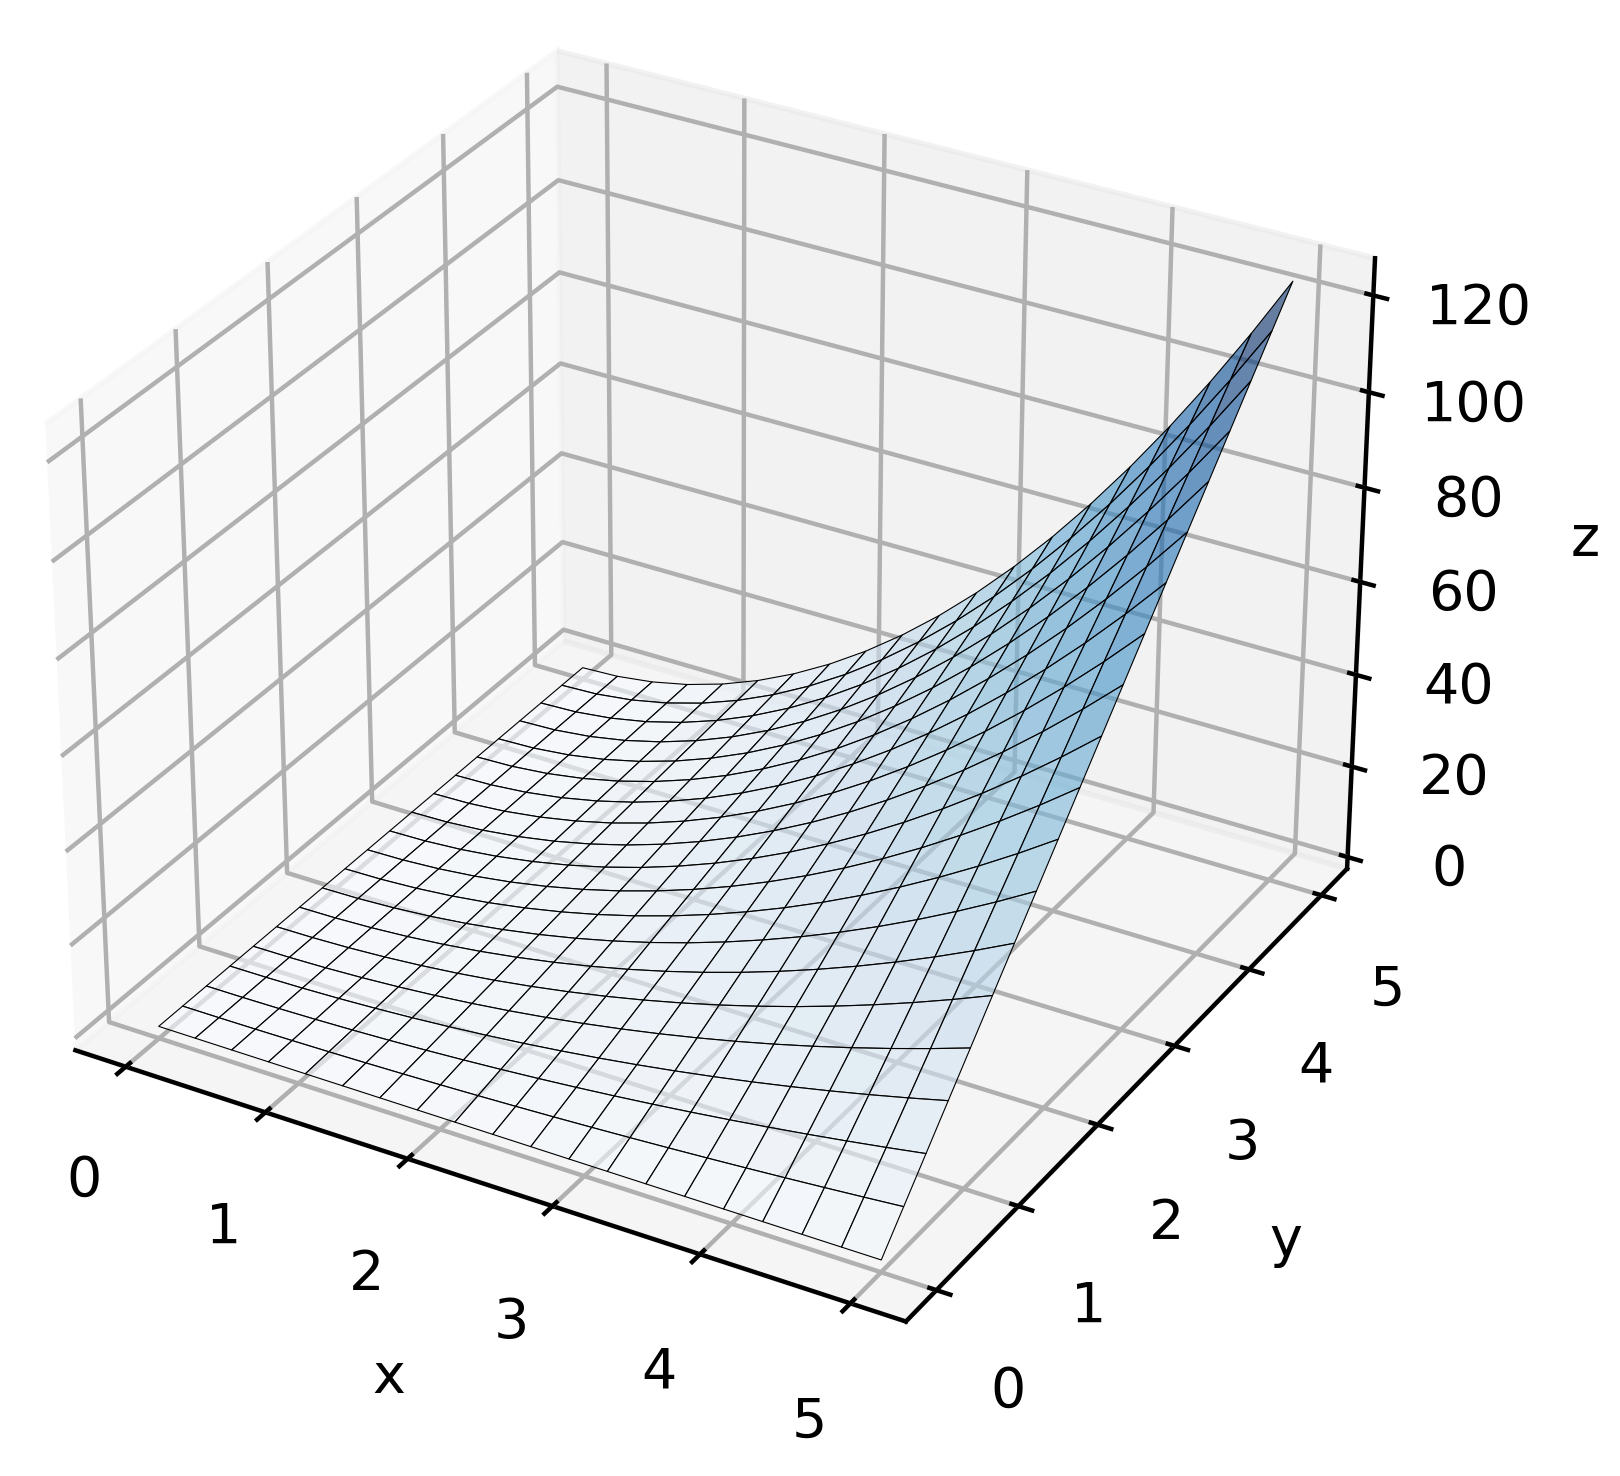
\includegraphics[scale=0.4]{figuras/der-parc2.png}
%\end{center}
%
%\end{minipage}
%
%\end{frame}
%


\begin{frame}
Se fixarmos $y=-3$ e deixarmos {\color{red}$x$} variar livremente, teremos uma função apenas da variável {\color{red}$x$}, cujo gráfico, é uma curva sobre a superfície do gráfico de de $f$.
\[f_1({\color{red}x})=f({\color{red}x},-3)=91-{\color{red}x^2}, \ -5\sqrt{2}\leq {\color{red}x}\leq 5\sqrt{2} \]

	
\begin{center}
	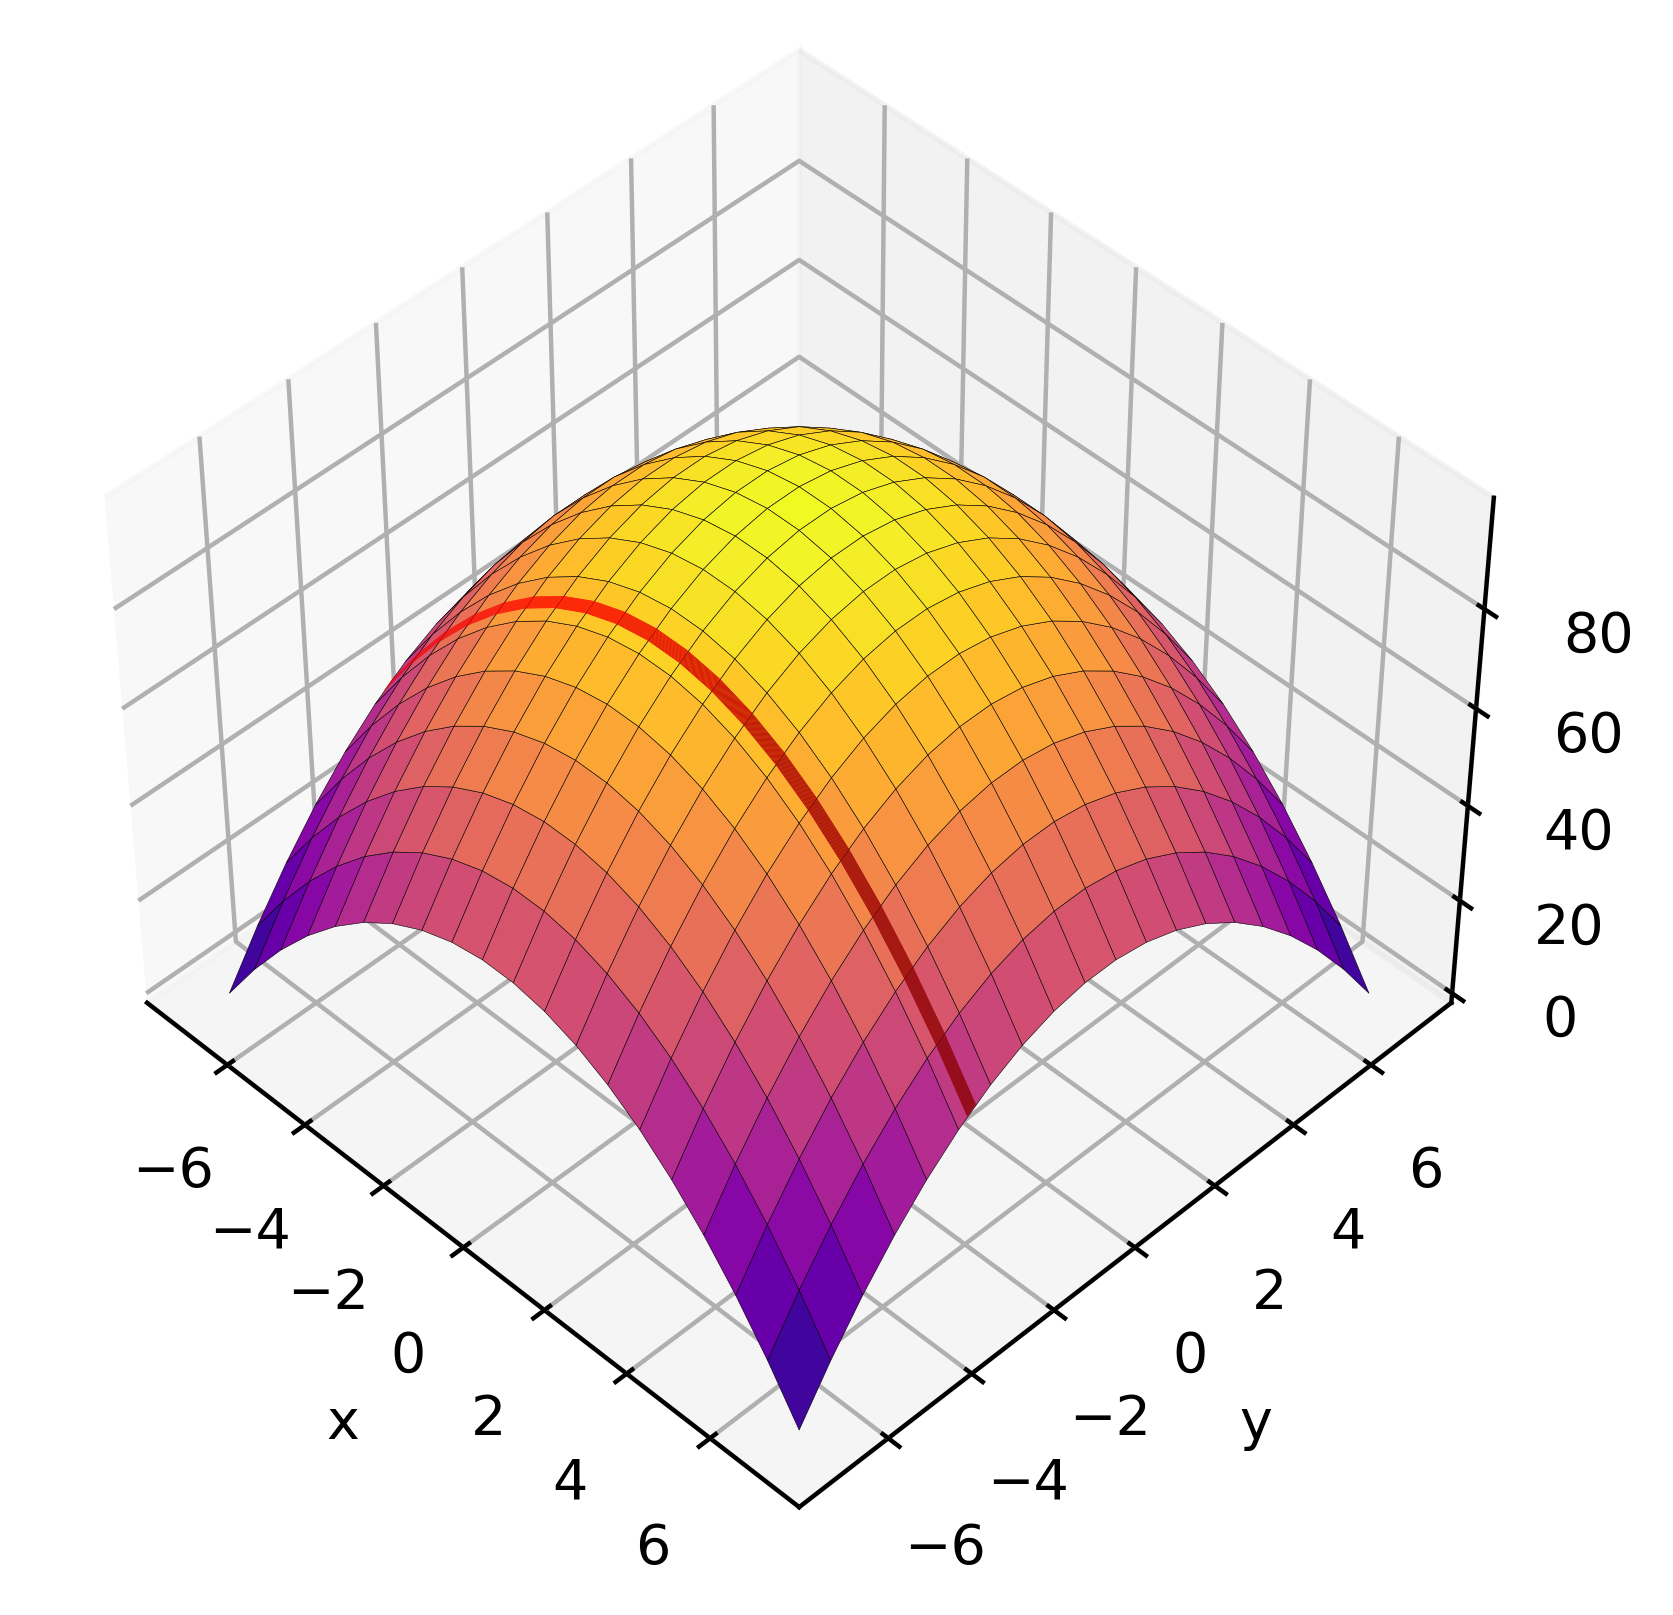
\includegraphics[scale=0.6]{figuras/der-parc2-2.png}
\end{center}
\end{frame}

\begin{frame}
	Analogamente, se fixarmos $x=2$ e deixarmos {\color{blue}$y$} variar livremente, teremos uma função apenas da variável {\color{blue}$y$}, cujo gráfico, é uma curva sobre a superfície do gráfico de de $f$.
	\[f_2({\color{blue}y})=f(2,{\color{blue}y})=96-{\color{blue}y^2}, \ -5\sqrt{2}\leq {\color{blue}y}\leq 5\sqrt{2} \]
	
	
	\begin{center}
		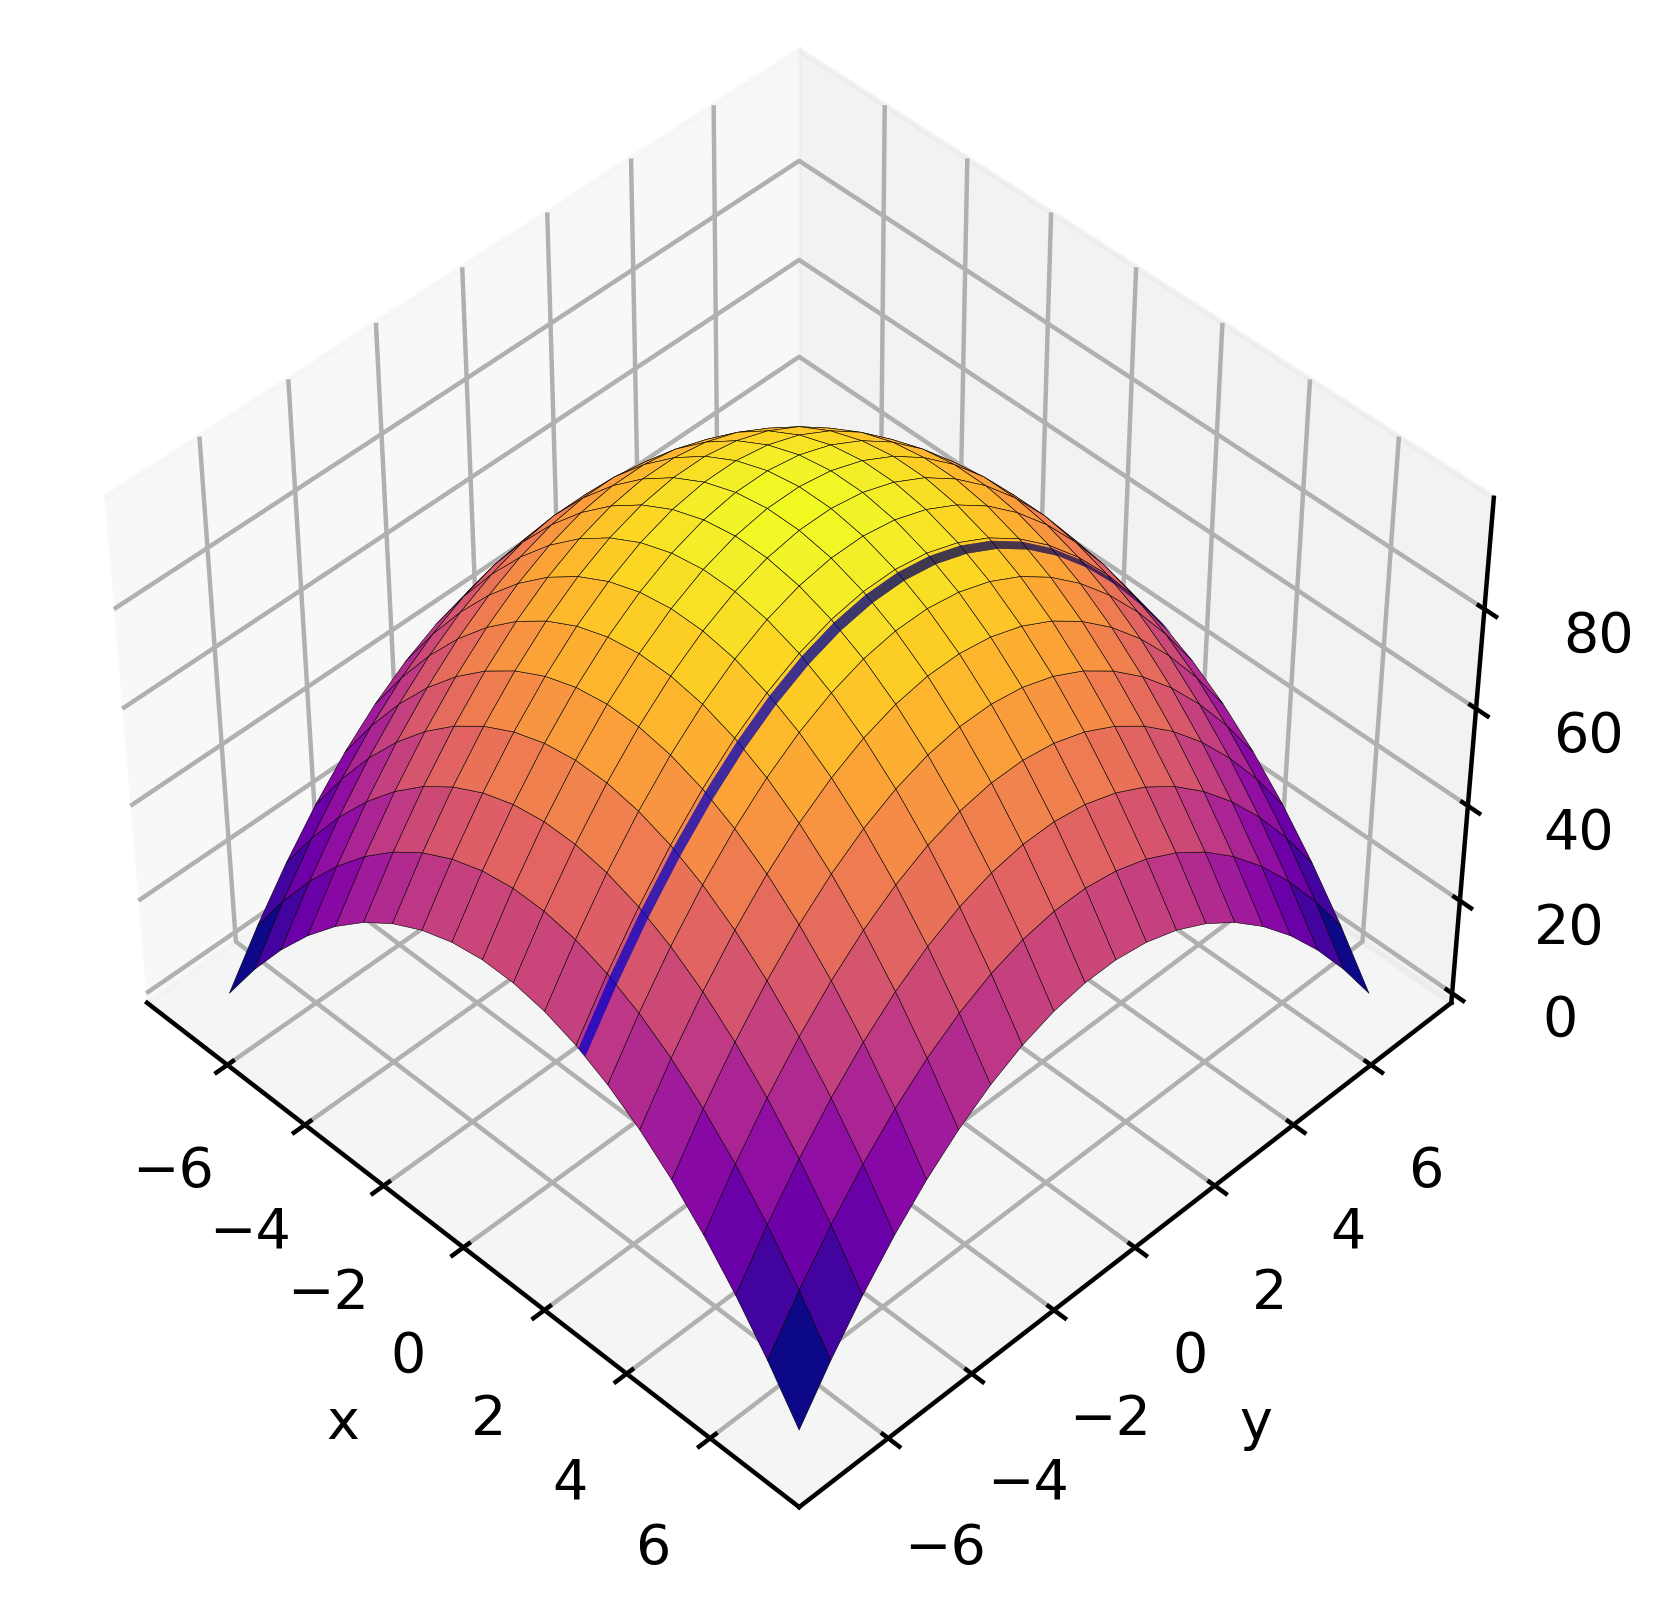
\includegraphics[scale=0.6]{figuras/der-parc2y-2.png}
	\end{center}
\end{frame}

\begin{frame}
	Em resumo, temos
	\[f_1({\color{red}x})=f({\color{red}x},-3)=91-{\color{red}x^2}, \ -5\sqrt{2}\leq {\color{red}x}\leq 5\sqrt{2} \]
	
	\[f_2({\color{blue}y})=f(2,{\color{blue}y})=96-{\color{blue}y^2}, \ -5\sqrt{2}\leq {\color{blue}y}\leq 5\sqrt{2} \]
	
	
	\begin{center}
		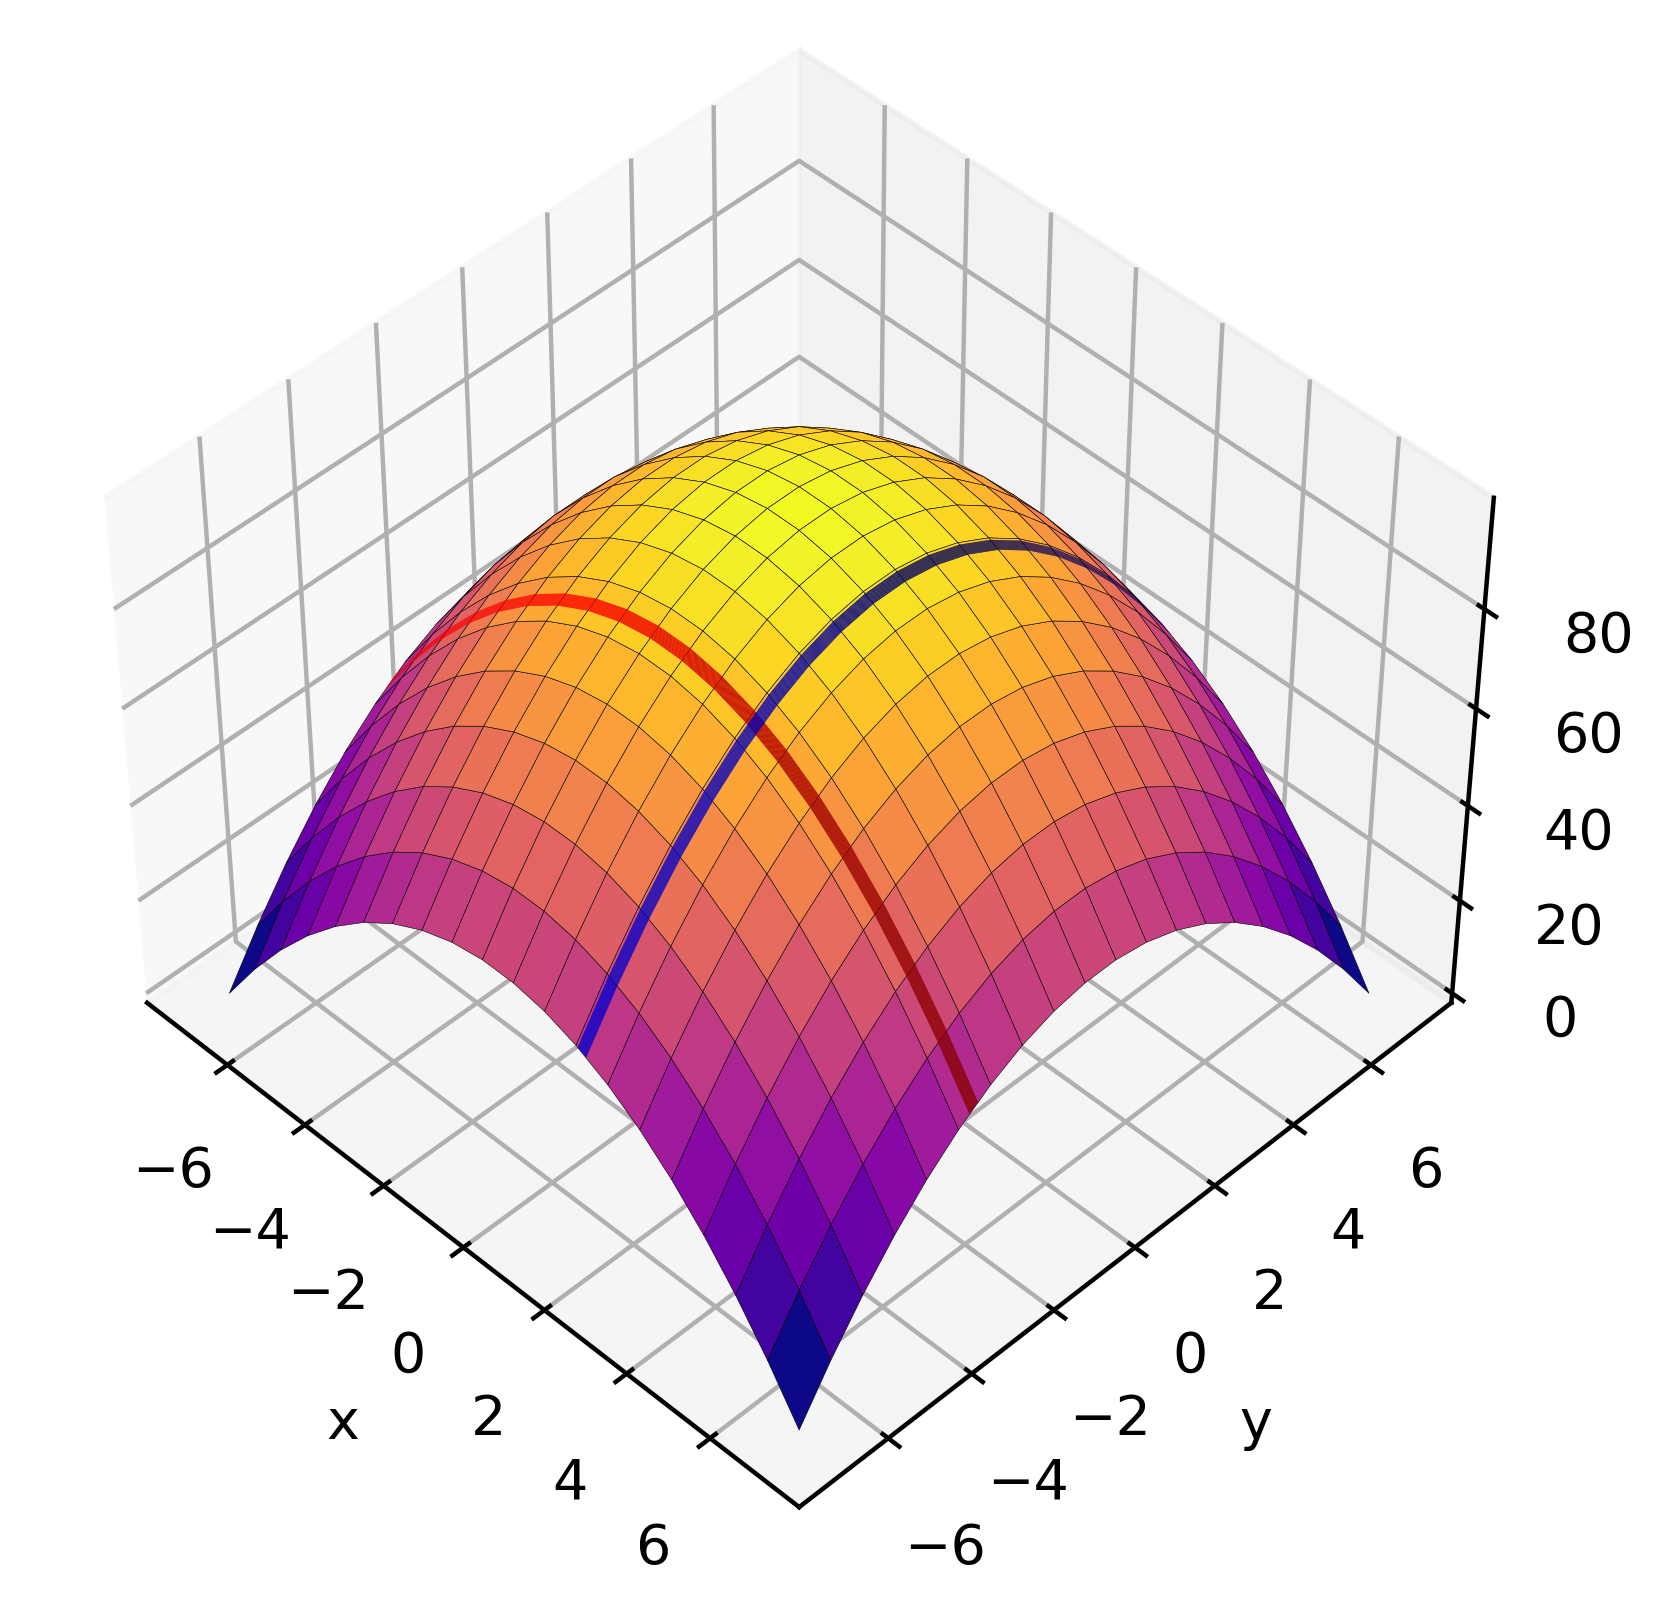
\includegraphics[scale=0.6]{figuras/der-parc2xy-2.png}
	\end{center}
\end{frame}

\begin{frame}
	É fácil ver que $f_1'({\color{red}x})=-2{\color{red}x}$. Assim, por exemplo, $f_1'(2)=-4$.
	\medskip 
	
	 Isso nos diz que a {\color{red}taxa de variação da temperatura}, no ponto $P=(2,-3)$, é de $-4^\circ C/m$ na {\color{blue}direção positiva do eixo $x$}.
	\medskip
	
	Em outras palavras, se caminharmos sobre a placa, a partir do ponto $P=(2,-3)$, {\color{blue}direção positiva do eixo $x$}, {\color{red}a temperatura vai cair a uma taxa de $-4^\circ C/m$.}
	
\begin{center}
	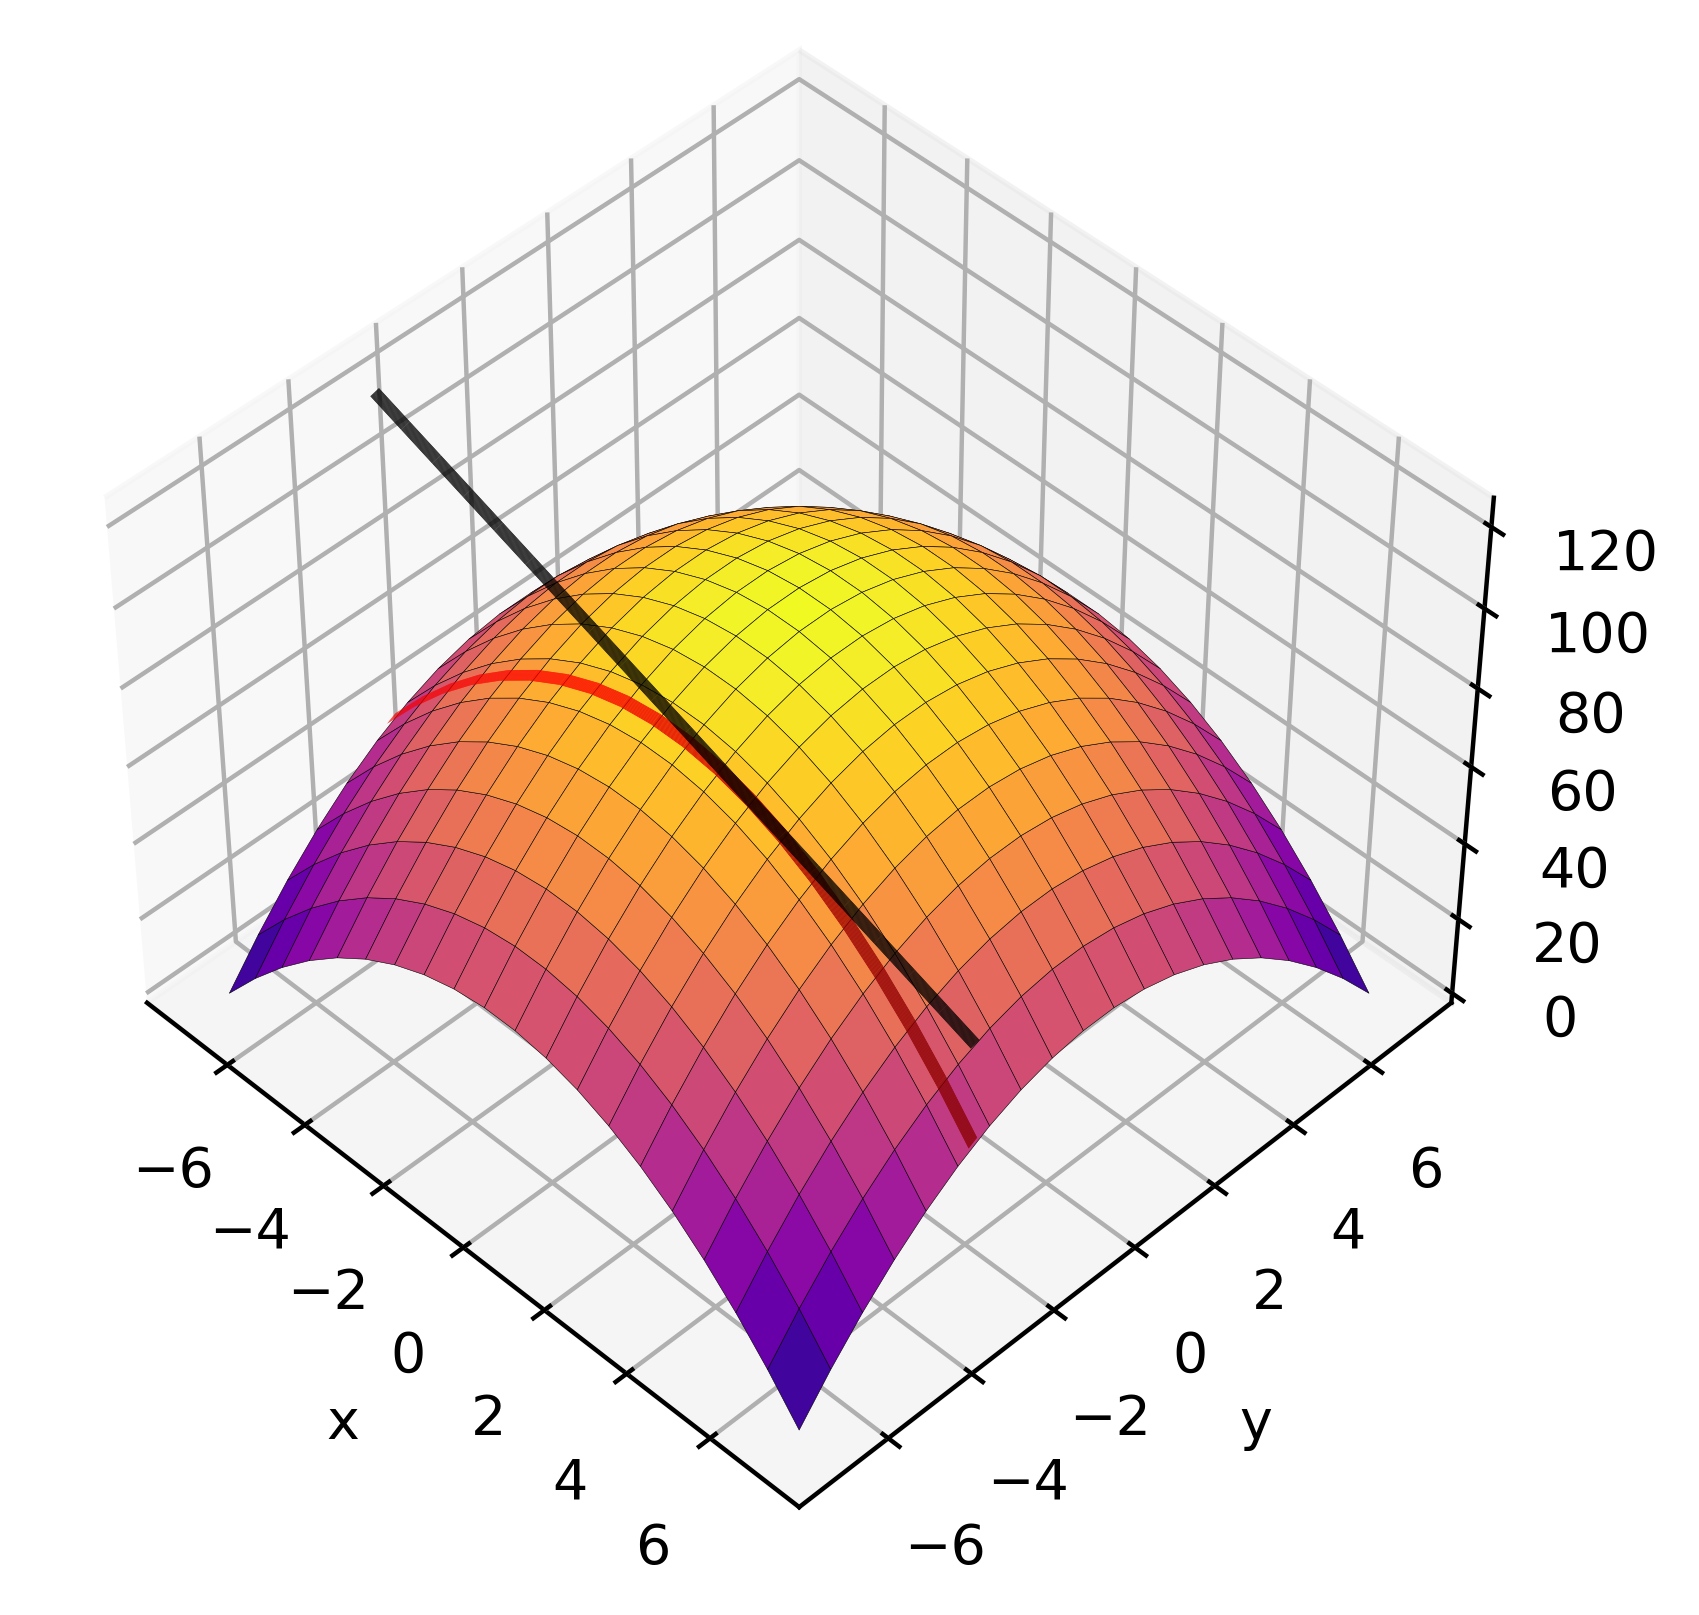
\includegraphics[scale=0.55]{figuras/der-parc2-3.png}
\end{center}
\end{frame}





\begin{frame}[label=der-parciais]
Sabemos que a derivada de $f_1$ em um ponto {\color{red} $a$} é dada por:
\[f_1'({\color{red}a})=\lim\limits_{h\to0}\frac{f_1({\color{red}a}+h)-f_1({\color{red}a})}{h}=\lim\limits_{h\to0}\frac{f({\color{red}a}+h,-3)-f({\color{red}a},2)}{h}.\]
\end{frame}


\begin{frame}[label=der-parciais]
	Sabemos que a derivada de $g$ em um ponto {\color{red} $a$} é dada por:
	\[f_1'({\color{red}a})=\lim\limits_{h\to0}\frac{f_1({\color{red}a}+h)-f_1({\color{red}a})}{h}=\lim\limits_{h\to0}\frac{f({\color{red}a}+h,-3)-f({\color{red}a},2)}{h}.\]
	De modo geral, se fixarmos um ponto genérico $y=b$, fazendo $f_1({\color{red}x})=f({\color{red}x},b)$, teremos:
	\[f_1'({\color{red}a})=\lim\limits_{h\to0}\frac{f_1({\color{red}a}+h)-f_1({\color{red}a})}{h}=\lim\limits_{h\to0}\frac{f({\color{red}a}+h,b)-f({\color{red}a},b)}{h}.\]
	Analogamente, se fixarmos um ponto genérico $x=a$, fazendo $f_2({\color{blue}y})=f(a,{\color{blue}y})$, teremos:
	\[f_2'({\color{blue}b})=\lim\limits_{h\to0}\frac{f_2({\color{blue}b}+h)-f_2({\color{blue}b})}{h}=\lim\limits_{h\to0}\frac{f(a,{\color{blue}b}+h)-f(a,{\color{blue}b})}{h}.\]
\end{frame}

\subsection*{Definição}
\begin{frame}[label=der-parciais]
%	\begin{scriptsize}
		\frametitle{}
		\uncover<1->{\begin{defin} Sejam $f:U\subset\R^2\to \R$ uma função e $(a,b)\in U$. A \dt{derivada parcial de $f$ em relação a $x$} no ponto $(a,b)$ é dada por
				$$\dx{f}(a,b)=\lim_{h\to 0}\frac{f(a+h,b)-f(a,b)}{h},$$
				quando este limite existe. Analogamente, A \dt{derivada parcial de $f$ em relação a y} no ponto $(a,b)$ é dada por
				$$\dy{f}(a,b)=\lim_{h\to 0}\frac{f(a,b+h)-f(a,b)}{h},$$
				quando este limite existe. 
		\end{defin}}
		
\begin{exe}
Se $f(x,y)=x^3+x^2y^3-2y^2$, determine $f_x(2,1)$ e $f_y(2,1)$.
\end{exe}
%	\end{scriptsize}
\end{frame}


\begin{frame}[label=der-parciais]
	\frametitle{ }
	Analogamente se $f:U\subset\R^3\to \R$ uma função definida em um aberto $U$ contendo $(x_0,y_0,z_0)$. As derivadas parcial de $f$ em relação a $x$, $y$ e $z$  no ponto $(x_0,y_0,z_0)$ são dadas pelos limites
\[\dx{f}(x_0,y_0,z_0)=\lim_{h\to 0}\frac{f(x_0+h,y_0,z_0)-f(x_0,y_0,z_0)}{h},\]
\[\dy{f}(x_0,y_0,z_0)=\lim_{h\to 0}\frac{f(x_0,y_0+h,z_0)-f(x_0,y_0,z_0)}{h},\]
\[\dz{f}(x_0,y_0,z_0)=\lim_{h\to 0}\frac{f(x_0,y_0,z_0+h)-f(x_0,y_0,z_0)}{h},\]
	quando estes limites existem. 
	
\begin{exe}
Se $f(x,y,z)=e^{xy}\log(z)$, determine as derivadas parciais.
\end{exe}
	
\end{frame}


\begin{frame}[label=der-parciais]
\begin{casa}
\begin{enumerate}
\item Se $f(x,y)=\sin\left(\frac{x}{1+y}\right)$, calcule $f_x$ e $f_y$.

\item Se $f(x,y,z)=x\sin(y-z)$, determine as derivadas parciais.
\end{enumerate}
\end{casa}
\end{frame}



\subsection*{Derivadas de Ordem Superior}
\begin{frame}[label=der-parciais]
	\frametitle{Derivadas de Ordem Superior }
%	\begin{scriptsize}
		
		\uncover<1->{ Se $z=f(x,y)$ é uma função, então  $\dx{f}$ e $\dy{f}$ também são funções de duas variáveis e portanto  podemos definir quatro novas funções que são chamadas de \dt{derivadas parciais de segunda ordem de f}, a saber:
			\begin{multicols}{2}
				$\dps f_{xx}=\frac{\partial^2f}{\partial x^2}=\dx{}\left(\dx{f}\right)$
				\bigskip
				
				$\dps f_{xy}=\frac{\partial^2f}{\partial y\partial x}=\dy{ }\left(\dx{f}\right)$
				\bigskip
				
				
				$\dps f_{yx}=\frac{\partial^2f}{\partial x\partial y}=\dx{}\left(\dy{f}\right)$
				\bigskip
				
				$\dps f_{yy}=\frac{\partial^2f}{\partial y^2}=\dy{}\left(\dy{f}\right)$
				\bigskip
		\end{multicols}}
		
		\uncover<1->{\begin{exe} Calcule todas as derivadas parciais de segunda ordem da função $f(x,y)=x^3+x^2y^3-2y^2$.
		\end{exe}}
		
		
%	\end{scriptsize}
\end{frame}




\begin{frame}[label=der-parciais]
	\frametitle{ }
	
\begin{teo} Se $z=f(x,y)$ é de classe $C^2$, então suas derivadas mistas são iguais, isto é, 
				$$\frac{\partial^2 f}{\partial x\partial y}=\frac{\partial^2 f}{\partial y\partial x}.$$
			\end{teo} 
			
%			\begin{exe} Calcule as derivadas mistas de $f$ no ponto $(0,0)$
%				$$f(x,y)=\left\{\begin{array}{ll}
%					\frac{xy^3}{x^2+y^2},& (x,y)\neq(0,0)\\
%					0, & (x,y)=(0,0)
%				\end{array}\right.$$
%		\end{exe}}
		
\end{frame}

\subsection*{EDPs}
\begin{frame}[label=der-parciais]{Equações Diferenciais Parciais - EDP}
As derivadas parciais ocorrem em {\color{blue}Equações Diferenciais Parciais} que exprimem certas leis físicas. Por exemplo, a EDP
\[u_{xx}+u_{yy}=0,\]
é chamada de {\color{blue} Equação de Laplace}. As soluções dessa equação são chamadas de {\color{blue} funções harmônicas}e são muito importantes no estudo de condução de calor, escoamento de fluidos e potencial elétrico.

\begin{exe}
Mostre que a função $u(x,y)=e^x\sin(y)$ é uma solução da equação de Laplace.
\end{exe}
\end{frame}

\begin{frame}[label=der-parciais]{Equação da Onda}
A {\color{blue}Equação da Onda}
\[u_{tt}=a^2u_{xx}\]
descreve o movimento de uma onda. Por exemplo, se $u(x,t)$ representa o deslocamento da corda vibrante de um violão no instante $t$ e à distância $x$ de uma das extremidades da corda, então $u(x,t)$ satisfaz a equação da onda. A constante $a$ depende da densidade da corda  e da tensão aplicada a nela.

\begin{exe}
Verifique que $u(x,t)=\sin(x-at)$ satisfaz a equação da onda.
\end{exe}
\end{frame}



\begin{frame}[label=der-parciais]
\begin{casa}
\begin{enumerate}
\item Calcule todas as derivadas parciais de segunda ordem da função $f(x,y)=xy-e^x\cos y$.
\item  Calcule $f_{xxyz}$ se $f(x,y,z)=\sin(3x+yz)$.
%
%
% Calcule $f_{zx}$ e $f_{xz}$ da função $f(x,y,z)=\log(x^2+y^2+z^2)$.
\end{enumerate}
\end{casa}
\end{frame}

%
%
%\begin{frame}[label=der-parciais]
%	\frametitle{ }
%	
%	\uncover<1->{\begin{exe}
%			%\begin{multicols}{3}
%			\begin{enumerate}
%				\item $f(x,y)=x^2+y$
%				\item $f(x,y,z)=xe^{x+y+z}$
%				\item $f(x,y)=\left\{\begin{array}{ll}
%					\frac{xy}{x^2+y^2},& (x,y)\neq (0,0)\\
%					0,& (x,y)= (0,0)\\
%				\end{array}\right.$
%			\end{enumerate}
%			%\end{multicols}
%	\end{exe}}
%	
%	\uncover<2->{Sabemos que se $f$ é uma função de uma variável derivável em $x_0$, então $f$ é contínua é contínua em $x_0$.}
%	\bigskip
%	
%	\uncover<3->{\textcolor{red}{Pergunta: Se $f$ é uma função de duas variáveis com derivadas parciais em $(x_0,y_0)$, então $f$ é contínua?! }}
%	
%\end{frame}

\subsection*{Aproximação Linear}

\begin{frame}[label=der-parciais]
	\frametitle{Aproximação Linear em uma variável}
%	\begin{scriptsize}
Em funções de uma variável sabemos que se {\color{blue}$f(x)$ é derivável em $x_0$}, sabemos que a reta tangente ao gráfico de $f$ no ponto $(x_0,f(x_0))$ é dada por
			\[L(x)=f(x_0)+f'(x_0)(x-x_0).\]
			Assim, para pequenos acréscimos $\Delta x$ na quantidade $x_0$, o valor de $f(x_0+\Delta x)$ é aproximadamente $L=f(x_0)+f'(x_0)\Delta x$, com erro
			\[E(\Delta x)=f(x_0+\Delta x)-f(x_0)-f'(x_0)\Delta x,\]
			onde {\color{red}$\dps\lim_{\Delta x\to 0}\frac{E(\Delta x)}{\Delta x}=0.$} Em outras palavras, o erro $E$ é menor que o erro $\Delta x$, para valores pequenos de $\Delta x$.
			
			
			Neste caso dizemos que $f$ é {\color{blue} diferenciável} e  que 
\[{\color{red}L(x)=f(x_0)+f'(x_0)(x-x_0)}\]
é uma {\color{red} aproximação linear} de $f$ no ponto $x_0$.
		
%		\uncover<1->{Com isso, para ver que $f$ é contínua em $x_0$ basta calcular o seguinte limite
%			$$\lim_{h\to 0}f(x_0+h)=\lim_{h\to 0}(f'(x_0)h+f(x_0)+E(h))=f(x_0)$$}
		
%	\end{scriptsize}
\end{frame}


\begin{frame}[label=der-parciais]
	\frametitle{Plano Tangente }
%	\begin{scriptsize}
		
		\uncover<1->{Como podemo obter o plano tangente ao gráfio da função  {\color{blue}$f(x,y)=9-x^2-y^2$} no ponto $P=(1,2,4)$?  }
		\bigskip 
		
Fixando  $y=2$ e fazendo $x$ variar, temos a curva sobre o gráfico passando por $P$
\[{\color{red}\alpha(x)=(x,2,5-x^2),\ x\in \R.}\]
cujo  o vetor tangente em $P$ é
\[{\color{red}u=\alpha'(1)=(1,0,-2).}\] 
Analogamente obtemos que outro vetor tangente ao gráfico no ponto $P$ é
\[{\color{cyan}v=(0,1,-4)}.\] 
Como {\color{cyan}$u$} e {\color{red}$v$} são LI, sabemos que o produto vetorial é um vetor normal ao plano, daí, obtemos que a equação do plano tangente é 
			\[2x+2y+z-10=0.\]
	
		
%	\end{scriptsize}
\end{frame}


\begin{frame}[label=der-parciais]
No caso geral, se $z=f(x,y)$, então o \dt{plano tangente} no ponto $P=(x_0,y_0,z_0)$ é dado pela equação
\begin{equation}\label{plano_tang}
{\color{blue}z=f(x_0,y_0)+\dx{f}(x_0,y_0)(x-x_0)+\dy{f}(x_0,y_0)(y-y_0).}
\end{equation}
O plano tangente é a {\color{red} melhor aproximação linear} da função {$z=f(x,y)$}	nas proximidades do ponto $P=(x_0,y_0,z_0)$ e a função 
\[{\color{red}L(x,y)=f(x_0,y_0)+\dx{f}(x_0,y_0)(x-x_0)+\dy{f}(x_0,y_0)(y-y_0)}\]
é denominada {\color{red}linearização} de $f$ no ponto $(x_0,y_0)$. 
\bigskip

\begin{alertblock}{ }
Diferentemente do caso unidimensional, para que essa aproximação seja boa, {\color{red}não é suficiente} que apenas existam as derivadas parciais. Para isso, precisamos definir uma noção de diferenciabilidade análoga.
\end{alertblock}
			
\end{frame}







\subsection*{Diferenciabilidade}
\begin{frame}[label=der-parciais]
	\frametitle{ }
%	\begin{scriptsize}
		
		\uncover<1->{\begin{defin}
				Uma $f:U\to \R$, definida no aberto $U\subset \R^2$, é dita \dt{diferenciável
				 em $(x_0,y_0)\in U$} quando existem $\dx{f}(x_0,y_0)$, $\dy{f}(x_0,y_0)$ tais que a função erro definida por 
\begin{multline*}
 E(\Delta x,\Delta y)=\\
 f(x_0+\Delta x,y_0+\Delta y)-f(x_0,y_0)-\dx{f}(x_0,y_0)\Delta x-\dy{f}(x_0,y_0) \Delta y,
\end{multline*}
satisfaz, $\displaystyle\lim_{(\Delta x,\Delta y)\to(0,0)}\frac{E(\Delta x,\Delta y)}{\|(\Delta x,\Delta y)\|}=0$
		\end{defin}}
		
\begin{alertblock}{ }
Esta definição diz que uma função diferenciável é aquela para a qual a aproximação linear é uma boa aproximação quando $(x,y)$ está próximo de $(x_0,y_0)$.
\end{alertblock}
	
\end{frame}

\begin{frame}[label=der-parciais]
\begin{exe}
Mostre que $f(x,y)=2x^2+y^2$ é diferenciável em $(1,1)$ e determine a aproximação linear.
\end{exe}

\begin{exe}
Mostre que a função $f(x,y)=x^{1/3}y^{1/3}$, possui derivadas parciais no ponto $(0,0)$ mas não é diferenciável, isto é, a equação do que seria o plano tangente existe, mas não fornece uma boa aproximação.
\end{exe}
\end{frame}


%
%\begin{frame}
%		\uncover<1->{\begin{teo} 
%				Se $f$ é diferenciável em $(x_0,y_0)$, então $f$ é contínua em $(x_0,y_0)$.
%		\end{teo}}
%		
%		\uncover<1->{Com essa definição podemos precisar o que é uma função ser ``suave''. Assim, podemos dizer que uma função é \dt{suave} quando existe o plano tangente ao gráfico da função, ou seja, quando $f$ é diferenciável. Note que  }
%%	\end{scriptsize}
%\end{frame}


\begin{frame}[label=der-parciais]
%	\frametitle{ }
%	\uncover<1->{\begin{exe}
%			\begin{enumerate}
%				\item Mostre que $f(x,y)=x^2+y^2$ é diferenciável em $\R^2$.
%				\item $f(x,y)=\left\{\begin{array}{ll}
%					\frac{x^2y}{x^4+y^2},&(x,y)\neq(0,0)\\
%					0, &(x,y)=(0,0)\\
%				\end{array}\right.$ é diferenciável em $(0,0)$?
%			\end{enumerate}
%	\end{exe}}
	
	\uncover<1->{\begin{defin} Uma função $f:U\to \R$, definida em um aberto $U\subset\R^2$, é dita de {\color{blue}classe $C^1$ em $U$} quando possui derivadas parciais contínuas em $U$. 
	\end{defin}}
	
	\uncover<1->{\begin{teo}\label{teo_dif} Se $f:U\to \R$ é de classe $C^1$ em $U$, então $f$ é diferenciável em $U$.
	\end{teo}}
	
	\begin{exe}
	Mostre que $f(x, y) = xe^{xy}$ é diferenciável em $(1, 0)$ e encontre sua linearização ali. Em seguida, use a linearização para aproximar $f( 1.1,-0.1)$.
	\end{exe}
\end{frame}


\subsection*{Diferenciais}
\begin{frame}[label=der-parciais]{Diferenciais}
Para uma função diferencial de uma única variável, $y = f(x)$, definimos a diferencial $dx$ como uma variável independente, ou seja, $dx$ pode valer qualquer número real. {\color{blue}A diferencial de $y$} é definida como
\[dy=f'(x) dx\]
\begin{center}
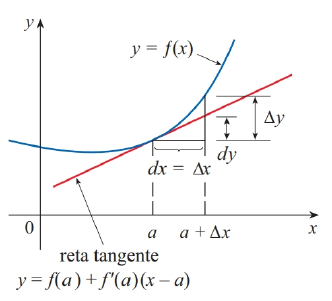
\includegraphics[scale=0.5]{figuras/diferenciais1.png}
\end{center}
\end{frame}

\begin{frame}[label=der-parciais]
Para uma função de duas variáveis, $z = f (x, y )$, definimos as diferenciais $dx$ e $dy$ como
variáveis independentes. Então, a {\color{blue}diferencial $dz$}, também chamada de {\color{blue} diferenciação total}, é definida por
\[dz
=\frac{\partial z}{\partial x}dx+\frac{\partial z}{\partial y}dy
=f_x(x,y)dx+f_y(x,y)dy\]
\begin{center}
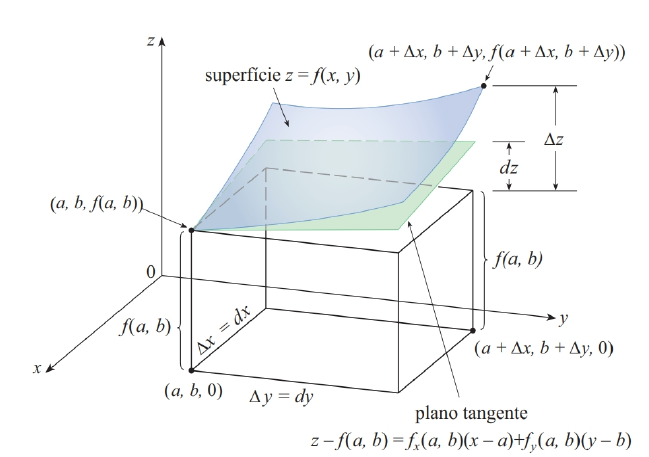
\includegraphics[scale=0.4]{figuras/diferenciais2.png}
\end{center}

\end{frame}

\begin{frame}[label=der-parciais]
\begin{exe}
Foram feitas medidas do raio da base e da altura de um cone circular reto e obtivemos 10 cm e 25 cm, respectivamente, com possível erro nessas medidas de, no máximo, $\varepsilon$ cm.
\begin{enumerate}
\item Use diferenciais para estimar o erro máximo cometido no cálculo do volume do
cone.

\item Se o raio e a altura forem medidos com erro máximo de 0.1 cm, qual será o erro máximo estimado para o volume? Estime o erro relativo.
\end{enumerate}
\end{exe}
\end{frame}

\begin{frame}[label=der-parciais]{Funções de três Variáveis}
Aproximações lineares, diferenciabilidade e diferenciais podem ser definidas de maneira análoga para as funções de mais que duas variáveis. 
\medskip


\begin{block}{Diferenciabilidade}
Uma função  $w=f(x,y,z)$ é {\color{blue} diferenciável em $(x_0,y_0,z_0)$} quando existem as derivadas parciais no ponto $(x_0,y_0,z_0)$ e 
\begin{multline*}
 E(\Delta x,\Delta y,\Delta z)=
 f(x_0+\Delta x,y_0+\Delta y,z_0+\Delta z)-f(x_0,y_0,z_0)\\-\dx{f}(x_0,y_0,z_0)\Delta x-\dy{f}(x_0,y_0,z_0) \Delta y-\dz{f}(x_0,y_0,z_0)\Delta z,
\end{multline*}
satisfaz, $\displaystyle\lim_{(\Delta x,\Delta y,\Delta z)\to(0,0,0)}\frac{E(\Delta x,\Delta y,\Delta z)}{\|(\Delta x,\Delta y,\Delta z)\|}=0$
\end{block}



\end{frame}



\begin{frame}[label=der-parciais]
Se $w=f(x,y,z)$ é diferenciável em $(x_0,y_0,z_0)$, então 
\bigskip

A {\color{blue}linearização} de $f$ no ponto $(x_0,y_0,z_0)$. 
{\color{blue}\begin{multline*}
L(x,y,z)=f(x_0,y_0,z_0)+\dx{f}(x_0,y_0,z_0)(x-x_0)\\+\dy{f}(x_0,y_0,z_0)(y-y_0)+\dz{f}(x_0,y_0,z_0)(z-z_0)
\end{multline*}}

A {\color{blue}diferencial $dw$}  é definida por
{\color{blue}
\[dw=\dx{w}dx+\dy{w}dy+\dz{w}dz.\]}



\end{frame}


\begin{frame}[label=der-parciais]
	\frametitle{ }
	\uncover<1->{\begin{casa}
			\begin{enumerate}
				\item Para quais valores de $(x,y)$,  $f(x,y)=\log(x^2+y^2)$ é diferenciável é diferenciável? Justifique.
				\item Mostre que $f(x,y)=\left\{\begin{array}{ll}
					\frac{xy}{x^2+y^2},& (x,y)\neq (0,0)\\
					0,& (x,y)= (0,0)\\
				\end{array}\right.$ não é diferenciável em $(0,0)$ mas possui derivadas parciais em $\R^2$.
			\end{enumerate}
	\end{casa} }
	
%	\uncover<2->{\begin{obs} A recíproca do Teorema \ref{teo_dif} é falsa, ou seja, existem funções diferenciáveis que não são de classe $C^1$. Um exemplo é a função
%			$$f(x,y)=\left\{\begin{array}{ll}
%				(x^2+y^2)\sen\left(\frac{1}{x^2+y^2}\right), &  (x,y)\neq (0,0)\\
%				0, & (x,y)=(0,0)\\
%			\end{array} \right.$$ 
%	\end{obs}}
\end{frame}


%\begin{frame}
%	\frametitle{Aplicação Função de Cobb-Douglas}
%	\begin{scriptsize}
%		
%		\uncover<1->{ Considere que uma empresa cuja produção possa ser modelada pela
%			seguinte função de Cobb-Douglas: $f(x,y)=10x^{0,4}y^{0,6}$, onde $f(x,y)$ é o valor da produção (medido em milhares de reais), $x$ é o investimento feito em infra-estrutura e maquinário e $y$ é o investimento feito em mão-de-obra (ambos medidos em milhares de reais). A característica dessa função é que a produção de sua empresa depende mais de mão-de-obra do que da infra-estrutura e maquinário. No momento a empresa tem R\$ 100.000 investidos em infra-estrutura e R\$ 200.000 em mão-de-obra, portanto está produzindo o equivalente a R\$ 1.515.716. Com isso, pergunta-se:}
%		
%		\uncover<2->{\begin{enumerate}
%				\item Qual a variação da produção quando mantemos a quantidade de trabalho constante e variamos a quantidade de capital? E quanto é a variação da produção quando mantemos o capital constante?
%				
%				\item Imagine que a empresa tenha possibilidade de investir mais R\$ 10.000 em infra-estrutura ou mão-de-obra, qual será o ganho aproximado na produção em cada caso? Você como Engenheiro de Produção indicaria qual opção para a empresa?
%				
%				
%		\end{enumerate}}
%		
%		
%		
%	\end{scriptsize}
%\end{frame}


\subsection*{Regra da Cadeia e Vetor Gradiente}


\begin{frame}[label=der-parciais]
	\frametitle{Regra da Cadeia e Vetor Gradiente }
%	\begin{scriptsize}
		
		\uncover<1->{\begin{block}{Regra da Cadeia 1} Sejam $z=f(x,y)$ uma função diferenciável e $\alpha(t)=(x(t),y(t))$, $t\in I$ também  diferenciável, então a função composta $z(t)=f(\alpha(t))$ é diferenciável e				\[\frac{dz}{dt}=\dx{z}\frac{dx}{dt}+\dy{z}\frac{dy}{dt}
		\]	\end{block} 
			
		}
\begin{minipage}{0.6\textwidth}
\begin{exe}
Se $z=x^2y+3xy^4$, onde $x=\sin(2t)$ e $y=\cos(t)$, determine $\frac{dz}{dt}$ em $t=0$.
\end{exe}
\end{minipage}
\begin{minipage}{0.3\textwidth}
\begin{center}
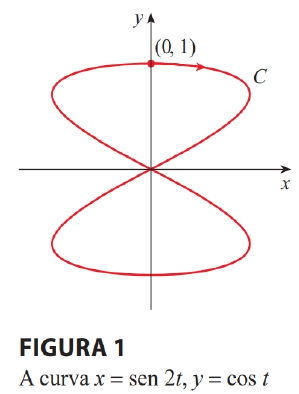
\includegraphics[scale=.4]{figuras/cadeia1.png}
\end{center}

\end{minipage}%	\end{scriptsize}
\end{frame}



%\begin{frame}
%	\frametitle{ }
%	\begin{scriptsize}
%		
%		\uncover<1->{\begin{exe}\begin{enumerate}
%					\item Sejam $z=f(x,y)=x^3y^2$, $x(t)=e^{-t}$ e $y(t)=t\sen t$. Calcule $\frac{dz}{dt}$.
%					
%					\uncover<2->{\item Certa vez, na logoa do Iriry, um grupo de estudantes de engenharia observou  que todos os dias, no mesmo horário, um pato partia de um ponto da lagoa e em 2 minutos atravessava a lagoa seguindo sempre uma mesma trajetória. 
%						\bigskip
%						
%						Determinados a entender os hábitos peculiares daquele pato, os estudantes construíram um sistema de coordenadas na lagoa, com origem no ponto de partida do pato e observaram que para cada ponto $(x,y)$ da lagoa poderiam associar uma função temperatura $T(x,y)$. Supondo que as temperaturas não variavam muito perto de um ponto da lagoa, assumiram que a função $T$ era diferenciável.  Além disso eles conseguiram descrever a trajetória do pato pela função $(x,y)=(t^2+1,3t)$ para cada instante $t$. Logo em seguida fizeram medições no lago e obtiveram que $T(5,6)=40$, $T_x(5,6)=4$, $T_y(5,6)=-2$. Com esses dados em mãos eles determinaram a taxa com que a temperatura variava em função do tempo no instante $t=2$. Qual é a taxa que eles obtiveram?}
%				\end{enumerate} 
%				
%		\end{exe} }
%		
%	\end{scriptsize}
%\end{frame}




\begin{frame}[label=der-parciais]
	\frametitle{ }
%	\begin{scriptsize}
\begin{minipage}{0.6\textwidth}
\begin{block}{Regra da Cadeia 2}
Sejam $z=f(x,y)$,  $x=x(t,s)$ e $y=y(t,s)$ são funções diferenciáveis, então
\begin{enumerate}[a]
	\item $\dps\frac{\partial z}{\partial s}={\color{red}\dx{z}}{\color{orange}\frac{\partial x}{\partial s}}+{\color{red}\dy{z}}{\color{orange}\frac{\partial y}{\partial s}}$
	\item $\dps\frac{\partial z}{\partial t}={\color{red}\dx{z}}{\color{cyan}\frac{\partial x}{\partial t}}+{\color{red}\dy{z}}{\color{cyan}\frac{\partial y}{\partial t}}$

		\end{enumerate} 
\end{block}
\end{minipage}\qquad
\begin{minipage}{0.3\textwidth}
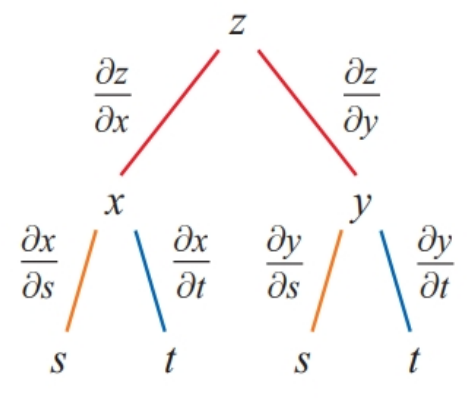
\includegraphics[scale=.3]{figuras/cadeia2.png}
\end{minipage}
\uncover<1->{\begin{exe} Calcule as derivadas parciais da função $z=e^x\sin(y)$, onde $x=st^2$ e $y=s^2t$
		\end{exe}}
		
%	\end{scriptsize}
\end{frame}



\begin{frame}[label=der-parciais]
	\frametitle{ }
%	\begin{scriptsize}
\begin{block}{Regra da Cadeia Caso Geral}
Sejam $u=u(x_1,x_2,\ldots,x_n)$ e $x_j=x_j(t_1,t_2,\ldots,t_m)$ funções diferenciáveis, então
\[\frac{\partial u}{\partial t_i}=\frac{\partial u}{\partial x_1}\frac{\partial x_1}{\partial t_i}+\frac{\partial u}{\partial x_2}\frac{\partial x_2}{\partial t_i}+\cdots +\frac{\partial u}{\partial x_n}\frac{\partial x_n}{\partial t_i}=\sum_{k=1}^{n}\frac{\partial u}{\partial x_k}\frac{\partial x_k}{\partial t_i}
\]
\end{block}

\uncover<1->{\begin{exe}
Se $u=x^4y+y^2z^3$, onde $x=rse^t$, $y=rs^2e^{-t}$ e $z=r^2s\sin(t)$, determine $\frac{\partial u}{\partial s}$ quando $r=2, s=1$ e $t=0$.
		\end{exe}}
		
%	\end{scriptsize}
\end{frame}


\begin{frame}[label=der-parciais]
\begin{casa}
\begin{enumerate}
\item Se $g(s,t)=f(s^2-t^2,t^2-s^2)$ e $f$ é diferenciável, mostre que $g$ satisfaz
\[t\frac{\partial g}{\partial s}+s\frac{\partial g}{\partial t}=0.\]

\item O raio de um cone circular reto está aumentando em uma taxa de 4.6 cm/s enquanto sua altura está descendo a uma taxa de 6.5 cm/s. Em qual taxa o volume do cone está variando quando o raio é 300 cm e altura é de 350 cm.
\end{enumerate}
\end{casa}
\end{frame}

\begin{frame}[label=der-parciais]
	\frametitle{ }
%	\begin{scriptsize}
		
		\uncover<1->{\begin{defin}Seja $f$ uma função de $n$ variáveis $x_1,\ldots,x_n$ que possui derivadas parciais no ponto $P_0=(a_1,\ldots,a_n)$. O \dt{vetor gradiente} de $f$ em $P_0$, denotado por $\nabla f(P_0)$, é o vetor
				$$\nabla f(P_0)=\left(\frac{\partial f}{\partial x_1},\ldots,\frac{\partial f}{\partial x_n}\right)$$
		\end{defin} }
		
		\uncover<1->{Usando a definição de vetor gradiente, a regra da cadeia pode ser escrita da forma
			$$\frac{dz}{dt}=\nabla f(\alpha(t))\cdot \alpha'(t).$$
			
			\begin{teo} Seja $z=f(x,y)$ uma função de classe $C^1$ definida em um aberto $U\subset \R^2$. O vetor gradiente é normal a qualquer curva de nível da função $f$ nos pontos em que não se anula.
		\end{teo}}
		
%	\end{scriptsize}
\end{frame}


\begin{frame}[label=der-parciais]
	\frametitle{ }
	
	\uncover<1->{O Teorema anterior também é válido para funções de três variáveis. Neste caso o vetor gradiente é normal à superfície de nível $F(x,y,z)=k.$ Este resultado pode ser usado para encontrar plano tangente à superfícies que não estão expressas como gráfico de função.
	
	\begin{center}
	\includegraphics[scale=0.4]{figuras/plano-tang.png}
	\end{center}
		
		\begin{exe} Determine  as equações do plano tangente e da reta normal à superfície $S$ de equação $x^2+3y^2+4z^2=8$ em $(1,-1,1)$.
	\end{exe} }
	
\end{frame}

\subsection*{Derivadas Direcionais em duas variáveis}


\begin{frame}[label=der-parciais]
	\frametitle{ Derivadas Direcionais}
%	\begin{scriptsize}
		
		\uncover<1->{\begin{defin} A \dt{derivada direcional} de uma função $z=f(x,y)$ em um ponto $P_0=(x_0,y_0)$ na direção do {\color{red}vetor unitário $u=(a,b)$}  é definida por
\begin{multline*}
\frac{\partial f}{\partial {\color{red}u}}(P_0)=\lim_{ {\color{blue}h}\to 0} \frac{f(P_0+{\color{blue}h}{\color{red}u})-f(P_0)}{{\color{blue}h}}
\\=\lim_{ {\color{blue}h} \to 0 } \frac{f(x_0+{\color{blue}h}{\color{red}a},y_0+{\color{blue}h}{\color{red}b})-f(x_0,y_0)}{{\color{blue}h}},
\end{multline*}
se este limite existir.
\end{defin} 
			
			\begin{teo} Se $z=f(x,y)$ é diferenciável em $P_0=(x_0,y_0)$, então 
				\[\frac{\partial f}{\partial u}(P_0)=\nabla f(P_0)\cdot u.\]
		\end{teo}}
		
		
%	\end{scriptsize}
\end{frame}

\begin{frame}[label=der-parciais]
A mesma definição e o último teorema valem para para funções de qualquer número de variáveis.


\uncover<1->{\begin{exe}
				Determine a derivada direcional da função $f$ no ponto $P$  na direção do vetor $v$ em cada caso:
				\begin{enumerate}
					\item $f(x,y)=x^2y^3-4y$, $P=(2,-1)$ e $v=(2,5)$.
					
					\item $f(x,y,z)=x\sen(yz)$, $P=(1,3,0)$ e $v=(1,2,-1)$.
				\end{enumerate} 
		\end{exe}}
		
		

		
\end{frame}

%\begin{frame}[label=der-parciais]
%	\frametitle{ Derivadas Direcionais em três ou mais variáveis}
%%	\begin{scriptsize}
%		
%		\uncover<1->{\begin{defin} A \dt{derivada direcional} de uma função $z=f(x,y,z)$ em um ponto $P_0=(x_0,y_0,z_0)$ na direção do {\color{red}vetor unitário $u=(a,b,c)$}  é definida por
%\begin{equation*}
%\frac{\partial f}{\partial {\color{red}u}}(P_0)=\lim_{ {\color{blue}h}\to 0} \frac{f(P_0+{\color{blue}h}{\color{red}u})-f(P_0)}{{\color{blue}h}}
%\end{equation*}
%se este limite existir.
%\end{defin} 
%			
%			\begin{teo} Se $z=f(x,y,z)$ é diferenciável, então 
%				\[\frac{\partial f}{\partial u}(P_0)=\nabla f(P_0)\cdot u.\]
%		\end{teo}}
%		
%		
%%	\end{scriptsize}
%\end{frame}



\begin{frame}[label=der-parciais]
	\frametitle{ }
%	\begin{scriptsize}
		
		\uncover<1->{\begin{teo} O valor máximo da derivada direcional de uma função diferenciável $f$ é a $\|\nabla f\|$ e ocorre na direção do vetor gradiente $\nabla f$.
			\end{teo} 
			
			\begin{exe} \begin{enumerate}
					\item Em que direção a função $f(x,y)=xe^y$ tem a maior taxa de variação? Qual é o valor da maior taxa de variação?
					
					\item Seja $T(x,y,z)=\dps\frac{80}{1+x^2+2y^2+3z^2}$ a temperatura, em graus Celsius, em um ponto $(x,y,z)$ do espaço. Em que direção no ponto $(1,1,-2)$ a temperatura aumenta mais rapidamente? Qual é a taxa máxima de aumento?
				\end{enumerate}
		\end{exe}}
		
%	\end{scriptsize}
\end{frame}

\begin{frame}[label=der-parciais]
\begin{block}{Propriedades do Vetor Gradiente}
Seja $f$ uma função diferenciável de duas ou três
variáveis e suponha que $\nabla f(P)\neq 0$.

\begin{itemize}
\item A derivada direcional de $f$ em $P$, na direção de um {\color{red}vetor unitário} $u$, é dada por
\[\frac{\partial f}{\partial u}(P)=\nabla f(P)\cdot u\]
\item $\nabla f(P)$ aponta na direção em que a taxa de crescimento de $f$ em $P$ é máxima e essa taxa máxima de variação é igual a $\|\nabla f(P)\|$

\item $\nabla f(P)$ é perpendicular à curva ou à superfície de nível de $f$ em $P$.
 \end{itemize}
\end{block}


\end{frame}

\begin{frame}[label=der-parciais]
\begin{center}
\begin{minipage}{0.5\textwidth}
\includegraphics[scale=.6]{figuras/grad1.png}
\end{minipage}\ \ \ \
\begin{minipage}{0.4\textwidth}
\includegraphics[scale=.6]{figuras/grad2.png}
\end{minipage}
\end{center}
\end{frame}

\subsection*{Teorema da Função Implícita}

\begin{frame}[label=der-parciais]{Diferenciação Implícita}
A função $F(x,y)=x^2+y^2$ tem como curvas de nível círculos centrados na origem.
\[x^2+y^2=k,\ k\geq 0.\]
 Sabemos que o círculo não é o gráfico de uma função de uma variável, entretanto, ao isolarmos uma das variáveis, ele pode ser visto como a união de dois gráficos:
 \[y=\pm\sqrt{k-x^2} \text{ ou } x=\pm\sqrt{k-y^2}\]
Entretanto, na maioria dos casos não é possível isolar uma das variáveis. Nestes casos, como podemos garantir que um pedaço da curva pode ser vista como gráfico de função? Ou dito de outra forma, como garantir que uma variável pode ser colocada em função das demais?
\end{frame}

\begin{frame}[label=der-parciais]{Teorema da Função Implícita I}
Suponha que 
\begin{enumerate}
\item A função $z=F(x,y)$ seja de {\color{blue}classe $C^1$};

\item $F(x_0,y_0)=0$ e ${\color{red}\dy{F}(x_0,y_0)\neq 0}$.
\end{enumerate}
Então, existe uma vizinhança $I$ em torno do ponto $x_0$ e uma {\color{blue}única} função $y=y(x)$ {\color{blue}também de classe $C^1$} tais que 
\[F(x,y(x))=0,\ \text{ para todo } x\in I \]
 e vale
 \[   {\frac{dy}{dx}}=\dps -\frac{\dx{F}}{{\color{red}{\dy{F}}}}.\] 

\begin{exe}
Mostre que $x^3+y^3-6xy=0$ define $y$ como função de $x$ na vizinhança do ponto $(3,3)$ e calcule $y'(3)$ a derivada neste ponto.
\end{exe}

\end{frame}


\begin{frame}[label=der-parciais]{Teorema da Função Implícita II}
Suponha que 
\begin{enumerate}
\item A função $F(x,y,z)$ seja de {\color{blue}classe $C^1$};

\item $F(x_0,y_0,z_0)=0$ e {\color{red}$\dz{F}(x_0,y_0,z_0)\neq 0$}.
\end{enumerate}
Então, existe uma vizinhança $U$ em torno do ponto $(x_0,y_0)$ e uma {\color{blue}única} função $z=z(x,y)$, {\color{blue} também de classe $C^1$}, tais que 
\[F(x,y,z(x,y))=0,\ \text{ para todo } (x,y)\in U \]
 e vale
 \[   \dx{z}=\dps -\frac{\dx{F}}{{\color{red}{\dz{F}}}}\text{ e }   \dy{z}=\dps -\frac{\dy{F}}{{\color{red}{\dz{F}}}}.\] 

%\begin{exe}
%Mostre que $z$ pode ser definida como uma função de $x$ e $y$ na vizinhança de $(0,0)$ para a equação
%\[x^3+z^2+ye^{xz}+z\cos(y)\]
%\end{exe}

\end{frame}


\begin{frame}[label=der-parciais]
\begin{exe}
Verifique que a equação $x^3+3y^2+8xz^2-3z^3y=9$ define $z$ com função de $x$ e $y$ numa vizinhança do ponto $(1,0,1)$ e calcule $\dps\frac{\partial z}{\partial x}(1,0)$, $\dps\frac{\partial z}{\partial y}(1,0)$ e $\dps\frac{\partial^2  z}{\partial y\partial x}(1,0)$.
\end{exe}
\end{frame}



\section{Extremos de Funções de Várias Variáveis}

\begin{frame}[label=otimizacao]{Valores Extremos de Funções de duas Variáveis }
%\begin{scriptsize}

\uncover<1->{ \begin{defin} \begin{enumerate}
\item Dizemos que uma função $f$ de duas variáveis tem um \dt{valor máximo local} no ponto $(a,b)$ se existir  uma bola aberta $B_r(a,b)$ tal que $f(a,b)\geq f(x,y)$ para todo $(x,y)\in B_r(a,b)$.

\item Dizemos que uma função $f$ de duas variáveis tem um \dt{valor mínimo local} no ponto $(a,b)$ se existir  uma bola aberta $B_r(a,b)$ tal que $f(a,b)\leq f(x,y)$ para todo $(x,y)\in B_r(a,b)$.
\end{enumerate}
\end{defin}}

\begin{center}
\includegraphics[scale=.4]{figuras/max-min1.png}
\end{center}

%\end{scriptsize}
\end{frame}


\begin{frame}[label=otimizacao]

\begin{teo} Se $f(x,y)$ tem um extremo local em $(a,b)$ e possui derivadas parciais em $(a,b)$, então 
\[\nabla f(a,b)=0.\]
\end{teo}

Um ponto $(a,b)$ tal que $\nabla f(a,b)$ não existe ou $\nabla f(a,b))=0$   é dito \dt{ ponto crítico ou ponto estacionário} de $f$.

\begin{minipage}{0.5\textwidth}
\begin{exe}
Determine os extremos relativos de $f(x,y)=x^2+y^2-2x-6y+14$
\end{exe}
\end{minipage}\ \
\begin{minipage}{0.3\textwidth}
\includegraphics[scale=.4]{figuras/pnt-critico.png}
\end{minipage}

\end{frame}


\begin{frame}[label=otimizacao]
\begin{exe} A função $f(x,y)=y^2-x^2$ tem ponto crítico em $(0,0)$ mas não possui extremo relativo!
 \end{exe} 
 \begin{minipage}{0.5\textwidth}
 \includegraphics[scale=.5]{figuras/sela.png}
 \begin{center}
 
 ponto de sela
 \end{center}
 \end{minipage}
  \begin{minipage}{0.2\textwidth}
  \includegraphics[scale=.4]{figuras/sela-montanha.png}
  \end{minipage}
\end{frame}


\subsection*{Matriz Hessiana}
\begin{frame}[label=otimizacao]
\frametitle{Matriz Hessiana }
%\begin{scriptsize}

Se $f$ é uma função de duas variáveis com todas as derivadas de ordem 2 no ponto $(a,b)$, definimos 
\[D^2f(a,b)=\left[\begin{array}{cc}
f_{xx}(a,b) & f_{xy}(a,b)\\
\\
f_{yx}(a,b) & f_{yy}(a,b)
\end{array}   \right],\]
chamada \dt{matriz Hessiana} da função $f$ no ponto $(a,b)$.



%\end{scriptsize}
\end{frame}

\subsection*{Teste da Segunda Derivada}
\begin{frame}[label=otimizacao]
\frametitle{Teste da Segunda Derivada}

\begin{teo}[Teste da Segunda Derivada]

Seja $z=f(x,y)$ uma função de classe $C^2$ em uma bola $B_r(a,b)$ tal que $\nabla f(a,b)=(0,0)$. Neste caso,
\begin{enumerate}[a]
\item Se $\det D^2f(a,b)>0$ e $f_{xx}(a,b)<0$, então $(a,b)$ é máximo local.

\item Se $\det D^2f(a,b)>0$ e $f_{xx}(a,b)>0$, então $(a,b)$ é mínimo local.

\item Se $\det D^2f(a,b)<0$, então $(a,b)$ é ponto de sela.


\end{enumerate}
\end{teo}

\begin{obs}
Se $\det D^2f(a,b)=0$, nada podemos concluir.
\end{obs}

%%\begin{exe} \begin{enumerate}
%%\item Localize e classifique os pontos críticos de $f(x,y)=2x^3+y^3-3x^2-3y$.
%%
%%\item O gráfico da função $g(x,y)=\frac{1}{xy}$ é uma superfície $S$ em $\R^3$. Encontre os pontos de $S$ mais próximos da origem.
%%\end{enumerate}
%\end{exe}



\end{frame}

\begin{frame}[label=otimizacao]
\begin{exe}
Localize e classifique os pontos críticos de $f(x,y)=x^4+y^4-4xy+1$.
\end{exe}
 \begin{minipage}{0.5\textwidth}
 \includegraphics[scale=.5]{figuras/teste-derv2.png}
 \begin{center}
 \end{center}
 \end{minipage}
  \begin{minipage}{0.2\textwidth}
  \includegraphics[scale=.4]{figuras/mapa-cont.png}
  \end{minipage}
\end{frame}

\begin{frame}[label=otimizacao]
\begin{casa}
Uma caixa retangular  sem tampa deve ser feita com 12 m$^2$ de papelão. Determine o volume máximo da caixa.
\end{casa}
\end{frame}


\subsection*{Máximos e Mínimos Absolutos}
\begin{frame}[label=otimizacao]
\frametitle{ }


\uncover<1->{\begin{defin}
Seja uma função $f$ de duas variáveis definida em um conjunto $U\subset \R^2$.
\begin{enumerate}


\item Dizemos que $f$  tem um valor \dt{máximo absoluto} em $U$ se existir um ponto $(a,b)\in U$ tal que $f(a,b)\geq f(x,y)$ para todo $(x,y)\in U$. Neste caso, $f(a,b)$ é {\color{red} o valor máximo absoluto }de $f$ em $U$. 

\item Dizemos que $f$  tem valor \dt{mínimo absoluto} em $U$ se existir um ponto $(a,b)\in U$ tal que $f(a,b)\leq f(x,y)$ para todo $(x,y)\in U$. Neste caso, $f(a,b)$ é {\color{red}o valor mínimo absoluto} de $f$ em $U$
\end{enumerate} 
\end{defin} 

\begin{exe} \begin{enumerate}
\item A função  $f(x,y)=1-x^2-y^2$ tem máximo absoluto em $\R^2$ no ponto $(0,0)$.

\item A função $f(x,y)=x$ não tem máximo nem mínimo absoluto em $\R^2$.
\end{enumerate} 
\end{exe}}



\end{frame}
\subsection*{Topologia no plano}
\begin{frame}[label=otimizacao]{Topologia no plano}
Antes de enunciarmos nosso próximo resultado, precisamos de algumas noções topológicas no plano.


\begin{minipage}{0.7\textwidth}
\begin{itemize}
\item Um conjunto é dito {\color{orange}limitado} se ele está contido em algum disco.

\item A \dt{fronteira} de um conjunto $D$, denotada por $\partial D$, é formada por pontos $(a,b)$ tais que qualquer disco aberto com centro em $(a,b)$ contém pontos de $D$ e pontos que não estão em $D$.


\item Um conjunto $D$ de $\R^2$ é dito \dt{fechado} se contém todos os pontos de sua fronteira, onde 

\item Um conjunto \dt{fechado} e {\color{orange}limitado} é dito ser \dt{compacto}.

\item Um conjunto  é {\color{red} aberto} quando seu complementar é fechado.


\end{itemize}

\end{minipage}
\begin{minipage}{0.2\textwidth}
\includegraphics[scale=.4]{figuras/fechados.png}
\end{minipage}



\end{frame}


\subsection*{Teorema de Weierstrass}
\begin{frame}[label=otimizacao]
\uncover<1->{\begin{teo}[Teorema de Weierstrass]
Se $f$ é uma {\color{red}função contínua} definida em um {\color{red}conjunto fechado e limitado} $D$ então $f$ {\color{blue}assume valor máximo e mínimo absolutos} em $U$.
\end{teo}}

\begin{exampleblock}{Determinação de Extremos Absolutos}
Para determinarmos os extremos absolutos de uma {\color{red}função contínua} definida em um {\color{red}conjunto fechado e limitado} $D$:
\begin{enumerate}
\item Determinar os valores de $f$ nos pontos críticos de $f$ em $D$.
\item Determinar os valores extremos de $f$ na fronteira de $D$.
\item O maior dos valores dos passos anteriores será o máximo absoluto e o menor deles o valor mínimo absoluto.
\end{enumerate}
\end{exampleblock}
\end{frame}

\begin{frame}[label=otimizacao]
\begin{exe}
Determine os valores extremos da função $f(x,y)=x^2-2xy+2y$ no retângulo $D=\{(x,y) |\ 0\leq x\leq 3, 0\leq y\leq 2 \}$.
\end{exe}

\begin{minipage}{0.45\textwidth}
\includegraphics[scale=0.5]{figuras/sec-15_7-fig13.png}
\end{minipage}
\begin{minipage}{0.45\textwidth}
\includegraphics[scale=0.5]{figuras/max1.png}
\end{minipage}
\end{frame}



%\begin{frame}
%\frametitle{ }
%\begin{scriptsize}
%
%\uncover<1->{\begin{exe}\begin{enumerate}
%\item Econtre o máximo e o mínimo da função $f(x,y)=(x-2)^2y+y^2-y$ definida em $D=\{(x,y)\in \R^2;\ x\geq 0, y\geq 0 \mbox{ e } x+y\leq 4\}$
%
%\item Uma placa metálica circular com um metro de raio está colocada com centro na origem do plano $xy$ e é aquecida de modo que a temperatura num ponto $(x,y)$ é dada por
%$$T(x,y)=64(3x^2-2xy+3y^2+2y+5),$$
%graus Celcius, onde $x,y$ estão em metros. Encontre a maior e a menor temperatura na placa.
%
%\end{enumerate} 
%\end{exe} }
%
%\end{scriptsize}
%\end{frame}




\subsection*{Multiplicadores de Lagrange}
\begin{frame}[label=otimizacao]
\frametitle{Multiplicadores de Lagrange  em duas Variáveis}


\begin{teo}Sejam $f(x,y)$ e $g(x,y)$ funções de classe $C^1$ definidas em um aberto $U$ que contém a curva $C$ de equação $g(x,y)=k$. Se $f(x,y)$ restrita à curva $C$ assume um valor máximo ou mínimo em $(x_0,y_0)\in C$ e {\color{red}$\nabla g(x_0,y_0)\neq \vec{0}$}, então existe {\color{blue}$\lambda\in \R$ }tal que
\[\nabla f(x_0,y_0)={\color{blue}\lambda} \nabla g(x_0,y_0)\]
\end{teo} 

\begin{center}
\includegraphics[scale=.5]{figuras/sec14_8-fig1.png}
\end{center}


\end{frame}


\begin{frame}[label=otimizacao]
\begin{exe}
Determine os valores extremos da função $f(x,y)=xy$ no círculo $x^2+y^2=1$.
\end{exe}

\begin{minipage}{0.55\textwidth}
\includegraphics[scale=.6]{figuras/exemplo-lagrange1.png}
\end{minipage}
\begin{minipage}{0.4\textwidth}
\includegraphics[scale=.45]{figuras/exemplo-lagrange-curvas-nivel.png}
\end{minipage}
\end{frame}

\begin{frame}[label=otimizacao]
\begin{casa}
Determine os pontos da hipérbole $x^2+8xy+7y^2-225=0$ que estão mais próximos da origem.
\end{casa}
\end{frame}

%\begin{exe}
%\begin{exe} \begin{enumerate}
%\item Determine os pontos extremos de $f(x,y)=xy$ tais que $x^2+y^2=1.$
%
%\item Determine os pontos extremos de $f(x,y)=x^2+2y^2$ tais que $x^2+y^2\leq 1.$
%
%
%\end{enumerate}
%\end{exe}
%\end{exe}


\begin{frame}[label=otimizacao]
\frametitle{ }
%\begin{scriptsize}
\begin{teo}Sejam $f(x,y,z)$ e $g(x,y,z)$ funções de classe $C^1$ definidas em um aberto $U$ que contém a superfície $S$ de equação $g(x,y,z)=k$. Se $f(x,y,z)$ restrita à superfície $S$ assume um valor máximo ou mínimo em $P_0=(x_0,y_0,z_0)\in S$ e $\nabla g(x_0,y_0,z_0)$ não é nulo, então existe $\lambda\in \R$ tal que
\[\nabla f(x_0,y_0,z_0)=\lambda \nabla g(x_0,y_0,z_0)\]
\end{teo} 

\begin{exe}
Determine os pontos da esfera $x^2+y^2+z^2=4$ que estão mais próximos e mais distantes do ponto $(3,1,-1)$.
\end{exe}

%\begin{exe} Encontre as dimensões da caixa retangular de maior volume que pode ser inscrita no elipsóide de equação $\dps \frac{x^2}{9}+\frac{y^2}{4}+z^2=1$, cujas arestas são paralelas aos eixos coordenados.
%\end{exe}}

%\end{scriptsize}
\end{frame}

\begin{frame}[label=otimizacao]
\frametitle{Multiplicadores de Lagrange com Duas Restrições}

\begin{teo}Sejam $f(x,y,z)$, $g_1(x,y,z)$ e $g_2(x,y,z)$  funções de classe $C^1$ definidas em um aberto $U$ que contém a curva $C$ de interseção das superfícies de equações $g_1(x,y,z)=k_1$ e $g_2(x,y,z)=k_2$. Se $f(x,y,z)$ restrita à curva  $C$ assume um valor máximo ou mínimo em $P_0=(x_0,y_0,z_0)\in S$ e $\nabla g_1(x_0,y_0,z_0)\times \nabla g_2(x_0,y_0,z_0)$ não é nulo, então existem $\lambda, \mu \in \R$ tais que
$$\nabla f(x_0,y_0,z_0)=\lambda \nabla g_1(x_0,y_0,z_0)+\mu \nabla g_1(x_0,y_0,z_0)$$ \end{teo} 

%\begin{exe} Encontre os pontos de máximo e mínimo de $f(x,y,z)=x+y+z$ sujeito às restrições $x^2+y^2=2$ e $x+z=1$.
%\end{exe}


\end{frame}


\begin{frame}[label=otimizacao]
\begin{exe}
Determine o valor máximo da função $f(x,y,z)=x+2y+3z$ na curva da interseção do plano $x-y+z=1$ com o cilindro $x^2+y^2=1$.
\end{exe}
\begin{center}
\includegraphics[scale=0.6]{figuras/sec14_8-fig8.png}
\end{center}
\end{frame}

\end{document}


